% !Mode:: "TeX:UTF-8"
%%%%%%%%%%%%%%%%%%%%%%%%%%%%%%%%%%%%%%%%%%%%%%%%%%%%%%%%%%%%%%%%%%%%%%%%%%%%%%%%
%          ,
%      /\^/`\
%     | \/   |                CONGRATULATIONS!
%     | |    |             SPRING IS IN THE AIR!
%     \ \    /                                                _ _
%      '\\//'                                               _{ ' }_
%        ||                     hithesis v3                { `.!.` }
%        ||                                                ',_/Y\_,'
%        ||  ,                   dustincys                   {_,_}
%    |\  ||  |\          Email: yanshuoc@gmail.com             |
%    | | ||  | |            https://yanshuo.name             (\|  /)
%    | | || / /                                               \| //
%    \ \||/ /       https://github.com/dustincys/hithesis      |//
%      `\\//`   \\   \./    \\ /     //    \\./   \\   //   \\ |/ /
%     ^^^^^^^^^^^^^^^^^^^^^^^^^^^^^^^^^^^^^^^^^^^^^^^^^^^^^^^^^^^^^^
%%%%%%%%%%%%%%%%%%%%%%%%%%%%%%%%%%%%%%%%%%%%%%%%%%%%%%%%%%%%%%%%%%%%%%%%%%%%%%%%
\documentclass[fontset=fandol,type=bachelor,campus=harbin]{hithesisbook}
% 此处选项中不要有空格
%%%%%%%%%%%%%%%%%%%%%%%%%%%%%%%%%%%%%%%%%%%%%%%%%%%%%%%%%%%%%%%%%%%%%%%%%%%%%%%%
% 必填选项
% type=doctor|master|bachelor|postdoc
%%%%%%%%%%%%%%%%%%%%%%%%%%%%%%%%%%%%%%%%%%%%%%%%%%%%%%%%%%%%%%%%%%%%%%%%%%%%%%%%
% 选填选项(选填选项的缺省值已经尽可能满足了大多数需求,除非明确知道自己有什么
% 需求)
% campus=shenzhen|weihai|harbin
%   含义:校区选项,默认harbin
% glue=true|false
%   含义:由于我工规范中要求字体行距在一个闭区间内,这个选项为true表示tex自
%   动选择,为false表示区间内一个最接近版心要求行数的要求的默认值,缺省值为
%   false。
% tocfour=true|false
%   含义:是否添加第四级目录,只对本科文科个别要求四级目录有效,缺省值为
%   false
% fontset=windows|mac|ubuntu|fandol|adobe
%   含义:设置字体,默认情况会自动识别系统,然后设置字体。后两个是开源字体,自行
%   下载安装后设置使用。windows是中易字库,窝工默认常用字体,绝对没毛病。mac和
%   ubuntu 默认分别是华文和思源字库,理论上用什么字库都行。后两种开源字库的安装
%   方法到谷歌上百度一下什么都有了。Linux非ubuntu发行版、非x86架构机器等如何运行
%   可到github issue上讨论。
% tocblank=true|false
%   含义:目录中第一章之前,是否加一行空白。缺省值为true。
% chapterhang=true|false
%   含义:目录的章标题是否悬挂居中,规范中要求章标题少于15字,所以这个选项
%   有无没什么用,除了特殊需求。缺省值为true。
% fulltime=true|false
%   含义:是否全日制,缺省值为true。非全日制如同等学力等,要在cover中设置类
%   型,封面中不同格式
% subtitle=true|false
%   含义:论文题目是否含有副标题,缺省值为false,如果有要在cover中设置副标
%   题内容,封面中显示。
% newgeometry=one|two|no
%   含义:规范中的自相矛盾之处,版芯是否包含页眉页脚,旧方法是按照包含页眉
%   页脚来设置。该选项是多选选项,如果设置为no,则版新为旧模板的版芯设置方法,
%   如果设置该选项one或two,分别对应两种页眉页码对应版芯线的相对位置。第一种
%   是严格按照规范要求,难看。第二种微调了页眉页码位置,好一点。默认two。
% debug=true|false
%   含义:是否显示版芯框和行号,用来调试。默认否。
% openright=true|false
%   含义:博士论文是否要求章节首页必须在奇数页,此选项不在规范要求中,按个
%   人喜好自行决定。 默认否。注意,窝工的默认情况是打印版博士论文要求右翻页
%   ,电子版要求非右翻页且无空白页。如果想DIY(或身不由己DIY)在什么地方右
%   翻页,将这个选项设置为false,然后在目标位置添加`\cleardoublepage`命令即
%   可。
% library=true|false
%   含义:是否为提交到图书馆的电子版。默认否。注意:如果设置成true,那么
%   openright选项将被强制转换为false。
% capcenterlast=true|false
%   含义:图题、表题最后一行是否居中对齐(我工规范要求居中,但不要求居中对
%   齐),此选项不在规范要求中,按个人喜好自行决定。默认否。
% subcapcenterlast=true|false
%   含义:子图图题最后一行是否居中对齐(我工规范要求居中,但不要求居中对齐
%   ),此选项不在规范要求中,按个人喜好自行决定。默认否。
% absupper=true|false
%   含义:中文目录中的英文摘要在中文目录中的大小写样式歧义,在规范中要求首
%   字母大写,在work样例中是全大写。该选项控制是否全大写。默认否。
% bsmainpagenumberline=true|false
%   含义:由于本科生论文官方模板的页码和页眉格式混乱,提供这个选项自定义设
%   置是否在正文中显示页码横线,默认否。
% bsfrontpagenumberline=true|false
%   含义:由于本科生论文官方模板的页码和页眉格式混乱,提供这个选项自定义设
%   置是否在前文中显示页码横线,默认否。
% bsheadrule=true|false
%   含义:由于本科生论文官方模板的页码和页眉格式混乱,提供这个选项自定义设
%   置是否显示页眉横线,默认显示。
% splitbibitem=true|false
%   含义:参考文献每一个条目内能不能断页,应广大刀客要求添加。默认否。
% newtxmath=true|false
%   含义:数学字体是否使用新罗马。默认是。
% chapterbold=true|false
%   含义:本科生章标题在目录和正文中是否加粗
% engtoc=true|false
%   含义:非博士生需要添加英文目录的,手动添加,如果是博士,此开关无效
% zijv=word|regu
%   含义:字距设置为规范规定33个字还是word中34个字。默认regu。
%%%%%%%%%%%%%%%%%%%%%%%%%%%%%%%%%%%%%%%%%%%%%%%%%%%%%%%%%%%%%%%%%%%%%%%%%%%%%%%%
\usepackage{hithesis}

\graphicspath{{./figures/}}

\begin{document}
\frontmatter
% !Mode:: "TeX:UTF-8"

\hitsetup{
  %******************************
  % 注意:
  %   1. 配置里面不要出现空行
  %   2. 不需要的配置信息可以删除
  %******************************
  %
  %=====
  % 秘级
  %=====
  statesecrets={公开},
  natclassifiedindex={TM301.2},
  intclassifiedindex={62-5},
  %
  %=========
  % 中文信息
  %=========
  ctitleone={基于抓取点生成网络与视},%本科生封面使用
  ctitletwo={觉伺服的未知物体抓取算法研究},%本科生封面使用
  ctitlecover={基于抓取点生成网络\\与视觉伺服的未知物体抓取算法研究},%放在封面中使用,自由断行
  ctitle={基于抓取点生成网络与视觉伺服的未知物体抓取算法研究},%放在原创性声明中使用
  csubtitle={一条副标题}, %一般情况没有,可以注释掉
  cxueke={工学},
  csubject={自动化},
  caffil={航天学院},
  cauthor={王泽飞},
  csupervisor={高会军},
  cassosupervisor={某某某教授}, % 副指导老师
  ccosupervisor={某某某教授}, % 联合指导老师
  % 日期自动使用当前时间,若需指定按如下方式修改:
  cdate={2022年6月x日},
  cstudentid={1181140118},
  cstudenttype={同等学力人员}, %非全日制教育申请学位者
  cnumber={no9527}, %编号
  cpositionname={哈铁西站}, %博士后站名称
  cfinishdate={20XX年X月---20XX年X月}, %到站日期
  csubmitdate={20XX年X月}, %出站日期
  cstartdate={3050年9月10日}, %到站日期
  cenddate={3090年10月10日}, %出站日期
  %(同等学力人员)、(工程硕士)、(工商管理硕士)、
  %(高级管理人员工商管理硕士)、(公共管理硕士)、(中职教师)、(高校教师)等
  %
  %
  %=========
  % 英文信息
  %=========
  etitle={Research on key technologies of partial porous externally pressurized gas bearing},
  esubtitle={This is the sub title},
  exueke={Engineering},
  esubject={Computer Science and Technology},
  eaffil={\emultiline[t]{School of Mechatronics Engineering \\ Mechatronics Engineering}},
  eauthor={Yu Dongmei},
  esupervisor={Professor XXX},
  eassosupervisor={XXX},
  % 日期自动生成,若需指定按如下方式修改:
  edate={December, 2017},
  estudenttype={Master of Art},
  %
  % 关键词用“英文逗号”分割
  ckeywords={\TeX, \LaTeX, CJK, 嗨!, thesis},
  ekeywords={\TeX, \LaTeX, CJK, template, thesis},
}

\begin{cabstract}

摘要的字数(以汉字计),硕士学位论文一般为500 $\sim$ 1000字,博士学位论文为1000 $\sim$ 2000字,
均以能将规定内容阐述清楚为原则,文字要精练,段落衔接要流畅。摘要页不需写出论文题目。
英文摘要与中文摘要的内容应完全一致,在语法、用词上应准确无误,语言简练通顺。
留学生的英文版博士学位论文中应有不少于3000字的“详细中文摘要”。

  关键词是为了文献标引工作、用以表示全文主要内容信息的单词或术语。关键词不超过 5
  个,每个关键词中间用分号分隔。(模板作者注:关键词分隔符不用考虑,模板会自动处
  理。英文关键词同理。)
\end{cabstract}

\begin{eabstract}
   An abstract of a dissertation is a summary and extraction of research work
   and contributions. Included in an abstract should be description of research
   topic and research objective, brief introduction to methodology and research
   process, and summarization of conclusion and contributions of the
   research. An abstract should be characterized by independence and clarity and
   carry identical information with the dissertation. It should be such that the
   general idea and major contributions of the dissertation are conveyed without
   reading the dissertation.

   An abstract should be concise and to the point. It is a misunderstanding to
   make an abstract an outline of the dissertation and words ``the first
   chapter'', ``the second chapter'' and the like should be avoided in the
   abstract.

   Key words are terms used in a dissertation for indexing, reflecting core
   information of the dissertation. An abstract may contain a maximum of 5 key
   words, with semi-colons used in between to separate one another.
\end{eabstract}
 % 封面
\makecover
\begin{denotation}
\begin{table}[h]%此处最好是h
\caption{国际单位制中具有专门名称的导出单位}
\vspace{0.5em}\centering\wuhao
\begin{tabular}{ccccc}
\toprule[1.5pt]
量的名称&单位名称&单位符号&其它表示实例\\
\midrule[1pt]
频率&赫[兹]&Hz&s-1\\
\bottomrule[1.5pt]
\end{tabular}
\end{table}
\end{denotation}
%物理量名称表,符合规范为主,有要求添加
\tableofcontents %目录
\mainmatter
%% !Mode:: "TeX:UTF-8"

\chapter[绪论]{Number}

研究生学位论文是研究生科学研究工作的全面总结,是描述其研究成果、代表其研究水平的
重要学术文献资料,是申请和授予相应学位的基本依据。学位论文撰写是研究生培养过程的
基本训练之一,必须按照确定的规范认真执行。研究生应严肃认真地撰写学位论文,指导教
师应加强指导,严格把关。

学位论文撰写应实事求是,杜绝造假和抄袭等行为;应符合国家及各专业部门制定的有关标
准,符合汉语语法规范。硕士和博士学位论文,除在字数、理论研究的深度及创造性成果等
方面的要求不同外,撰写规范要求基本一致。人文与社会科学、管理学科可在本撰写规范的
基础上补充制定专业的学术规范。

\section{课题背景及研究的目的和意义}[Content specification]


\section{机器人物体抓取的发展情况}[Content specification]



\section{本文的主要研究内容}[Content specification]





% Local Variables:
% TeX-master: "../main"
% TeX-engine: xetex
% End:













%%%%%%%%%%%%%%%%%%%%%%%%%%%%%%%%%绪论%%%%%%%%%%%%%%%%%%%%%%%%%%%%%%%%%
\chapter[绪论]{绪论}
\section{课题背景及研究的目的和意义}[Content specification]
要不看

\section{机器人视觉伺服系统概述}[Content specification]
分IBVS、PBVS和混合控制hvs。IBVS的基础原理从最原始的公式、解耦、图像矩到现在借助神经网络获直接端到端控制。绕不开当前特征与目标特征的提取的过程,但是方法越来越具有泛化性。
\section{基于视觉伺服的物体抓取发展现状}[Content specification]
抓取方法上:
经典的方法当然是人为的制作特征点或者标志,辅助视觉伺服。但是泛化性是不行的,需要避免人为的制作特征,让程序自主提取特征并生成目标。直接把整张图当作特征是后来的发展方向之一,这样必须要求目标与当前相似,伺服范围太小。神经网络兴起后,方法变得百花齐放。如现在不断发展的抓取合成(grasp systhesis),分经验法和深度法;神经网络自主生成目标图像但还是那个问题,这样必须要求目标与当前相似,伺服范围太小;手到眼系统,神经网络估计机械臂末端和目标的相对位姿,伺服后期会出现遮挡现象,一般还是要配合眼在手系统一起使用,涉及到多数据融合问题,非常复杂。通过渲染引擎获得目标图像,神经网络自动提取特征并匹配特征。大部分的方法无法回避需要线下制作目标图像的问题,对于一个完全未知的目标,如何在线上就能实时生成目标并执行抓取是对抓取未知目标任务的研究重点。
伺服性能上:
就算拥有一个合适的抓取方法,也需要有合适的控制律。低鲁棒性的伺服控制律,无法在应对各种位姿、形态的抓取对象中保证同样的抓取性能,这会大大降低最终的抓取成功率和伺服响应速度。为满足泛化性的需求,近几年有很多人投入到视觉伺服控制律的研究中,然后介绍各种控制方法。如何设计一个适合于当前抓取方法的控制律,是抓取未知目标任务的又一难点。


归功于近年深度网络的快速发展,抓取合成(grasp synthesis)的方法在这几年发展迅速。
\section{主要研究内容及章节安排}[Content specification]
介绍本文都要干些啥,IBVS相对于PBVS的优势,eye-to-hand系统
本文共分为六章,章节内容如下  
第一章:  
第二章:  
。。。





%%%%%%%%%%%%%%%%%%%%%%%%基于图像的视觉伺服理论研究%%%%%%%%%%%%%%%%%%%%%%%%%
\chapter[基于图像的视觉伺服(IBVS)理论研究]{基于图像的视觉伺服(IBVS)理论研究}
\section{引言}[Content specification]
绪论中介绍了IBVS相对于PBVS的优势:1.伺服精度不依赖于相机外参,深度鲁棒性强;2.直接得到指令,不需要轨迹规划,更易于实现实时闭环控制。因此认为IBVS更适合于未知位姿、形体的目标的抓取任务。IBVS作为本算法研究的基石之一,尤其需要十分严谨合理的模型建立、公式原理分析、完善的仿真系统和实物环境搭建,这会为之后的工作减少不少麻烦。本章中除了完成上述基础性工作,还在实物上成功运行了简单的基于特征点交互矩阵的IBVS。

\section{IBVS系统模型建立}[Content specification]
\subsection{系统坐标系建立}[Content specification]
对于IBVS系统,最需要关注的点有三个:机械臂末端、相机和目标。为了后续仿真程序实现和问题分析需要,建立系统的坐标系用于表述它们的位置。如图\ref{系统坐标系建立}所示:
\begin{figure}[h]
\centering
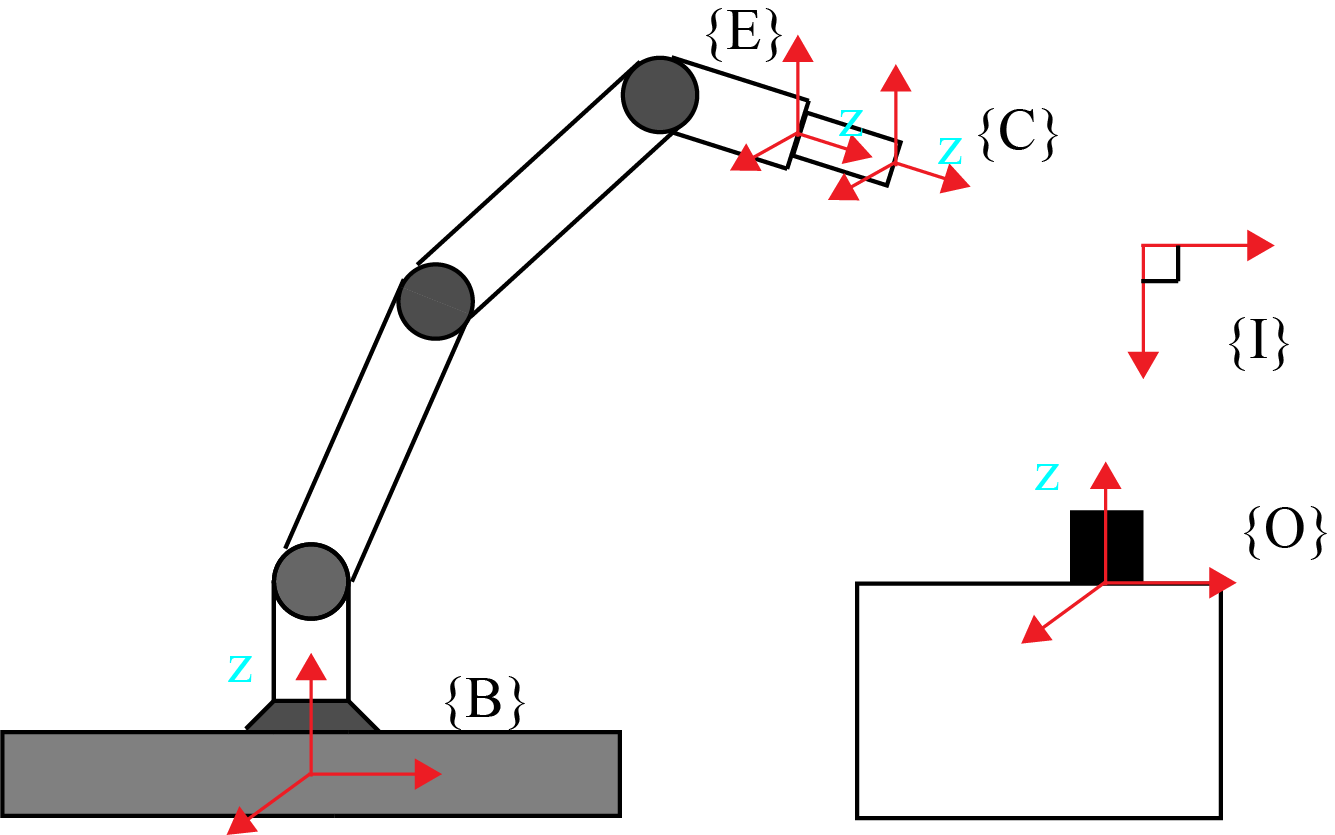
\includegraphics[width = 0.75\textwidth]{chapter2/系统坐标系建立}
\caption{系统坐标系建立示意图}
\label{系统坐标系建立}
\end{figure}

该示意图中,$\lbrace$\textit{O}$\rbrace$、$\lbrace$\textit{E}$\rbrace$和$\lbrace$\textit{C}$\rbrace$分别表示物体坐标系、机器人末端坐标系,eye-to-hand系统中的相机坐标系。为了便于阐述坐标变换公式,用$\lbrace$\textit{B}$\rbrace$、$\lbrace$\textit{I}$\rbrace$和$\lbrace$\textit{CI}$\rbrace$表示机器人基坐标系、图像坐标系和像素坐标系,本研究中所说的基坐标系和世界坐标系是一个意思。将使用以下符号表示各个相对位姿变换:
$^{B}T_O$表示目标$\lbrace$\textit{O}$\rbrace$相对于基坐标系$\lbrace$\textit{B}$\rbrace$的坐标变换;
$^{B}T_E$表示机器人末端$\lbrace$\textit{E}$\rbrace$相对于基坐标系$\lbrace$\textit{B}$\rbrace$的变换。对机械臂末端使用的速度指令是在这个变化下进行的;
$^{C}T_O$表示目标$\lbrace$\textit{O}$\rbrace$相对于相机坐标系$\lbrace$\textit{C}$\rbrace$的坐标变换;
$^{E}T_C$表示相机$\lbrace$\textit{C}$\rbrace$相对于末端坐标系$\lbrace$\textit{E}$\rbrace$的坐标变换。一般情况下IBVS的伺服结果是相机正对目标,而真正抓取还是要依赖末端位置,所以这个变换是必要的;
$^{C}T_I$表示图像$\lbrace$\textit{I}$\rbrace$相对于相机坐标系$\lbrace$\textit{C}$\rbrace$的坐标变换。特征初始是在图像中获取的,需要这个变换使特征位置描述变成IBVS需要的形式\cite{zh1}。


\subsection{视觉模型建立}[Content specification]
IBVS不断地由特征偏差驱动着运行,而对特征的描述需要在$^{C}T_O$下进行。在图像中获取的特征需要经过图\ref{特征变换}所示的坐标系变换才能真正为IBVS所用:
\begin{figure}[h]
\centering

\includegraphics[width = 0.60\textwidth]{chapter2/特征变换}
\caption{特征变换过程图}
\label{特征变换}
\end{figure}


不例外地使用针孔模型描述从像素坐标系到机器人基坐标系中物体的映射,这张图引自这篇文献\cite{zh1},这张针孔模型示意图十分典型。
\begin{figure}[h]
\centering
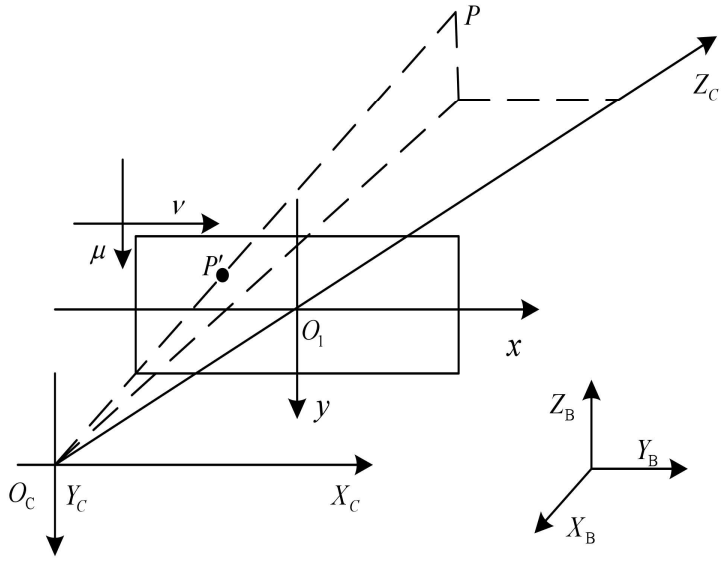
\includegraphics[width = 0.60\textwidth]{chapter2/视觉坐标系建立}
\caption{视觉坐标系建立示意图}
\label{视觉坐标系建立}
\end{figure}


图\ref{视觉坐标系建立}中用$X_CO_CY_C$描述$\lbrace$\textit{C}$\rbrace$,$xO_Iy$描述$\lbrace$\textit{I}$\rbrace$,P表示$\lbrace$\textit{C}$\rbrace$中的目标点,P'表示成像过程中投影到$\lbrace$\textit{I}$\rbrace$中的目标点。因为深度的存在,成像在二维像素坐标系中的图像所对应的目标可以是无穷多种情况,为了统一坐标变换形式,令目标深度$Z_C$为单位1,在相机坐标系$\lbrace$\textit{C}$\rbrace$和像素坐标系$\lbrace$\textit{CI}$\rbrace$中加上了一个过渡的图像坐标系$\lbrace$\textit{I}$\rbrace$。


相机内参由出厂地所给出,它包括相机的焦距$f$,相机放缩因子$f_x$和$f_y$,它们的单位为毫米;偏移量$c_x$和$c_y$,单位为像素,但是是浮点类型。由于Realsense D435i内置去畸变API,就不考虑畸变因素了。使用$\left[ u,v \right] ^T$表示像素坐标系下的目标点位置,$\left[ X_C,Y_C,Z_C \right] ^T$表示相机坐标系下的目标点位置,$Z_C$为相机深度,可以得到它们之间的关系:
\begin{equation}
	Z_C\left[ \begin{array}{c}
	\begin{array}{c}
	u\\
	v\\
\end{array}\\
	1\\
\end{array} \right] =\left[ \begin{matrix}
	f_x&		0&		c_x\\
	0&		f_y&		c_y\\
	0&		0&		1\\
\end{matrix} \right] \left[ \begin{array}{c}
	X_C\\
	Y_C\\
	Z_C\\
\end{array} \right] 
\label{像素到相机坐标变换} 
\end{equation} 


在已知相机内参的情况下,IBVS中所需要的特征位置描述就转换为找到特征对应的$\lbrace$\textit{CI}$\rbrace$中的位置$\left[ u,v \right] ^T$和深度相机测得对应点的深度$Z_C$。

\section{IBVS仿真系统实现}[Content specification]
\subsection{IBVS算法原理}[Content specification]
在本实验中所说的IBVS是基于特征点交互矩阵实现的\cite{chaumette2006visual}。它的基本思想是将特征点偏差通过交互矩阵(也叫图像雅可比矩阵)映射为末端速度指令。为了表述简洁,符号所代表的意思如下:$s^*=\left[ x^*,y^* \right] ^T$表示$\lbrace$\textit{C}$\rbrace$中对应的期望特征点坐标。$s=\left[ x,y \right] ^T$表示$\lbrace$\textit{C}$\rbrace$中对应的当前特征点坐标。$v_c=\left[ v_x,v_y,v_z,\omega _x,\omega _y,\omega _z \right] ^T$表示$\lbrace$\textit{B}$\rbrace$中相机的速度,其中相机包含质心线速度,和绕三个轴的角速度。由于相机和机械臂末端是固连且位置上接近的,所以它们的速度认为是一致的。使用交互矩阵$L_c$建立当前特征随时间变化率与相机位姿随时间变化率的关系:
\begin{equation}
\dot{s}=L_cv_c 
\label{当前特征变化率与相机位姿变化率的关系1} 
\end{equation} 


一般情况下,期望特征是不随时间改变的,或者变化甚微(在本研究中就是如此,所以进行近似),式\ref{当前特征变化率与相机位姿变化率的关系1}可以如方程组\ref{当前特征变化率与相机位姿变化率的关系2}中第一排表达式改写。另外,认为特征偏差随时间呈指数变化是合理的,因为它收敛快速且平滑\cite{chaumette2006visual},于是可以得到方程组\ref{当前特征变化率与相机位姿变化率的关系2}:
\begin{equation}
\left\{ \begin{array}{c}
	\left( \dot{s}-\dot{s}^* \right) =\dot{e}=L_cv_c\\
	L_e=L_c\\
	\dot{e}=-\lambda e\\
\end{array} \right.  
\label{当前特征变化率与相机位姿变化率的关系2} 
\end{equation} 


其中$\dot{e}$为当前特征偏差随时间变化率,$\lambda$为比例系数,$\dot{e}$为当前特征偏差。通过对交互矩阵求广义逆,由方程组\ref{当前特征变化率与相机位姿变化率的关系2}可得到:
\begin{equation}
\left\{ \begin{array}{c}
	v_c=-\lambda L_{e}^{+}e\\
	L_{e}^{+}=\left( L_{e}^{T}L_e \right) ^{-1}L_{e}^{T}\\
\end{array} \right. 
\label{当前特征变化率与相机位姿变化率的关系3} 
\end{equation} 


其中$\lambda L_{e}^{+}$为交互矩阵广义逆。通过方程组\ref{当前特征变化率与相机位姿变化率的关系3}可以借助当前特征偏差求取机器人末端速度了。交互矩阵由特征点在图像中的位置及深度信息得到,每个点对应的交互矩阵如式\ref{交互矩阵}所示,若有多个点,公式中的交互矩阵就是每个点对应的交互矩阵在行方向的叠加。
 \begin{equation}
L_e=\left[ \begin{matrix}
	\frac{-1}{Z_C}&		0&		\frac{X_C}{Z_C}&		X_CY_C&		-\left( 1+X_{C}^{2} \right)&		Y_C\\
	0&		\frac{-1}{Z_C}&		\frac{Y_C}{Z_C}&		1+Y_{C}^{2}&		-X_CY_C&		-X_C\\
\end{matrix} \right] 
\label{交互矩阵} 
\end{equation} 

\subsection{机器人仿真模型搭建}[Content specification]
基于为整个系统搭建的坐标系和不同系的坐标转换关系,借助ROS的moveit工具(由于ROS2的moveit2尚未开发成熟,使用moveit代替),为敬科公司提供的JK机器人搭建仿真模型。moveit是一个开发的十分完善的工具包,不仅实现了机械结构的仿真,物理模型、碰撞体积和逆运动学都在包中相应地实现。本研究中,为了能更快地验证提出的算法,减少繁杂的处理,将把物体放到一个平整且颜色单一(在后续的研究中可以发现这些要求都不是必须的)的表面上。另外,相机一直保持俯视朝下,在X、Y轴方向的角度保持为0°,因此速度指令中$\omega _x$和$\omega _y$不论结果计算如何都给0。仿真效果图如图\ref{基于moveit机器人仿真模型实现}所示。
\begin{figure}[h]
\centering
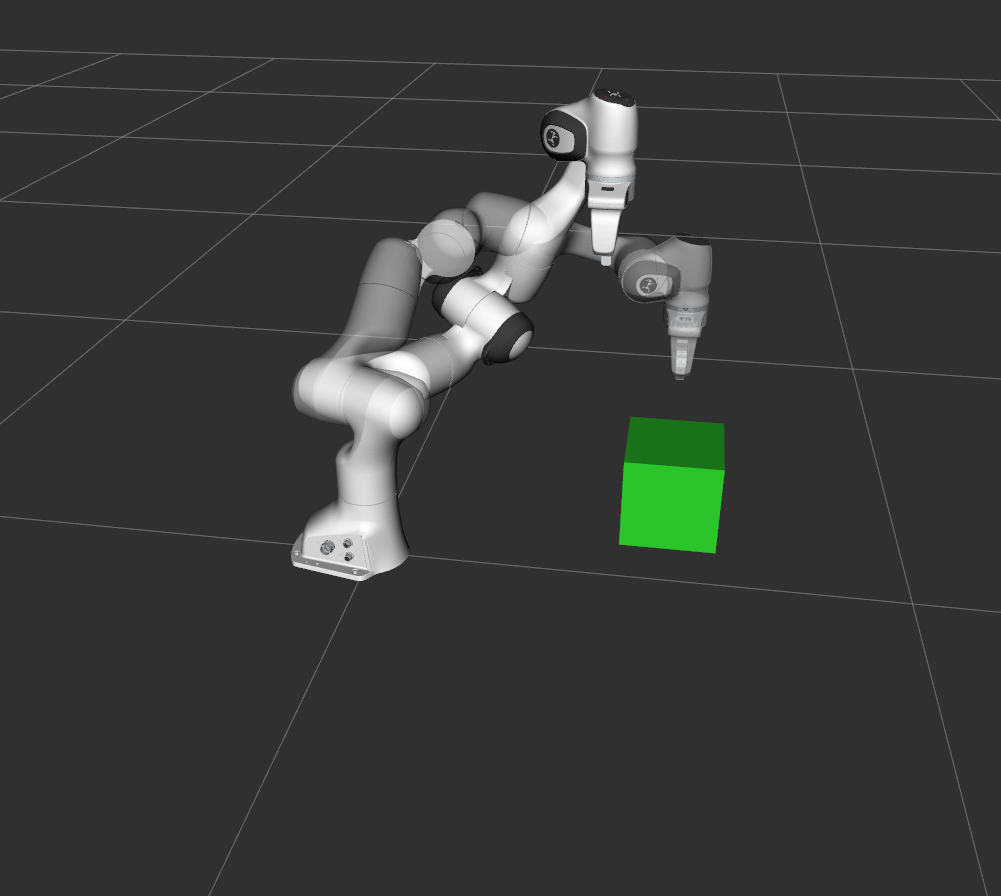
\includegraphics[width = 0.55\textwidth]{chapter2/基于moveit机器人仿真模型实现}
\caption{基于moveit机器人仿真模型实现}
\label{基于moveit机器人仿真模型实现}
\end{figure}


图\ref{IBVS基础控制流程方框图}展现了整个系统最基础的控制方框图,在实验进行过程中会不断被改进,以应对实践中发生的各个问题。
\begin{figure}[h]
\centering
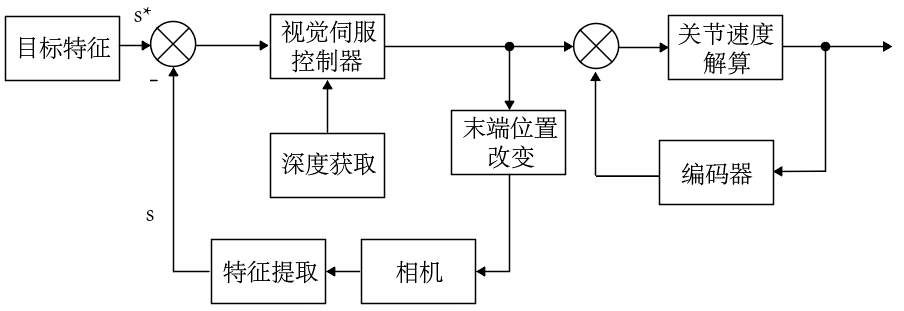
\includegraphics[width = 1.0\textwidth]{chapter2/IBVS基础控制流程方框图}
\caption{IBVS基础控制流程方框图}
\label{IBVS基础控制流程方框图}
\end{figure}


深度获取的方式是会根据深度条件切换的,如图\ref{深度传感器切换}所示。之所以加上这个切换,是因为Realsense D435i是基于结构光测量深度的,不可以测量过近距离的目标点。当相机在伺服末期十分靠近目标时,无法获得确切的目标点深度。所以在相机与目标点距离低于20cm时,会通过编码器读取末端下降的距离得到对应特征的深度,这在相机一直俯视向下时是可行的。


\begin{figure}[h]
\centering
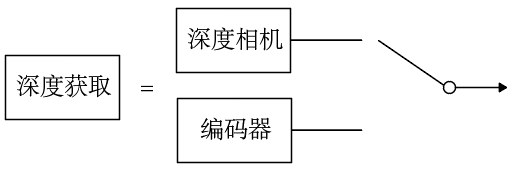
\includegraphics[width = 0.60\textwidth]{chapter2/深度选择图}
\caption{深度传感器切换示意图}
\label{深度传感器切换}
\end{figure}


开启仿真节点后,可以在另一个节点中与该节点建立连接并发送速度指令,仿真节点会因此响应,并进行移动。moveit有自己的限位系统,在机器人进入奇异点或者超出移动范围时给予及时的警告,所以该机器人仿真模型多被用于对机器人是否进入奇异点的判断这样的定性分析,后文中真正的调参还是在实物上进行的。
\subsection{曲线绘制与相机轨迹记录}[Content specification]
曲线是分析问题非常重要的一环,所以仿真中应当有相应的曲线绘制。IBVS本质是将特征偏差作为控制器输入而映射成速度指令的控制系统,所以研究中最关心的是点在于特征偏差和速度指令,它们将被分别绘制到两张图中。曲线图中时间单位为秒。关于特征偏差图:系统中定义特征偏差是相机坐标系中被检测的特征点在X、Y方向的偏差,单位为米,该单位不被展现在曲线中,因为它的单位并不重要。关于末端速度指令图:为了与JK机器人需要的末端速度指令单位保持一致,所以线速度选取厘米每秒为单位,而角速度单位则为度每秒。


直观地展现相机的位移情况也是重要的,因为IBVS往往对机器人末端的运动轨迹十分不友好。如果当前的速度指令使机器人颤振,那么机器人已经进入了一个十分糟糕的姿态,通过分析相机的运动轨迹适当调节控制律参数也是非常好的解决方法。调用VISP库,对设定的参数进行视觉伺服仿真,实现的曲线绘制和相机轨迹绘制效果如图\ref{基于VISP视觉伺服仿真}所示。
\begin{figure}[h]
\centering
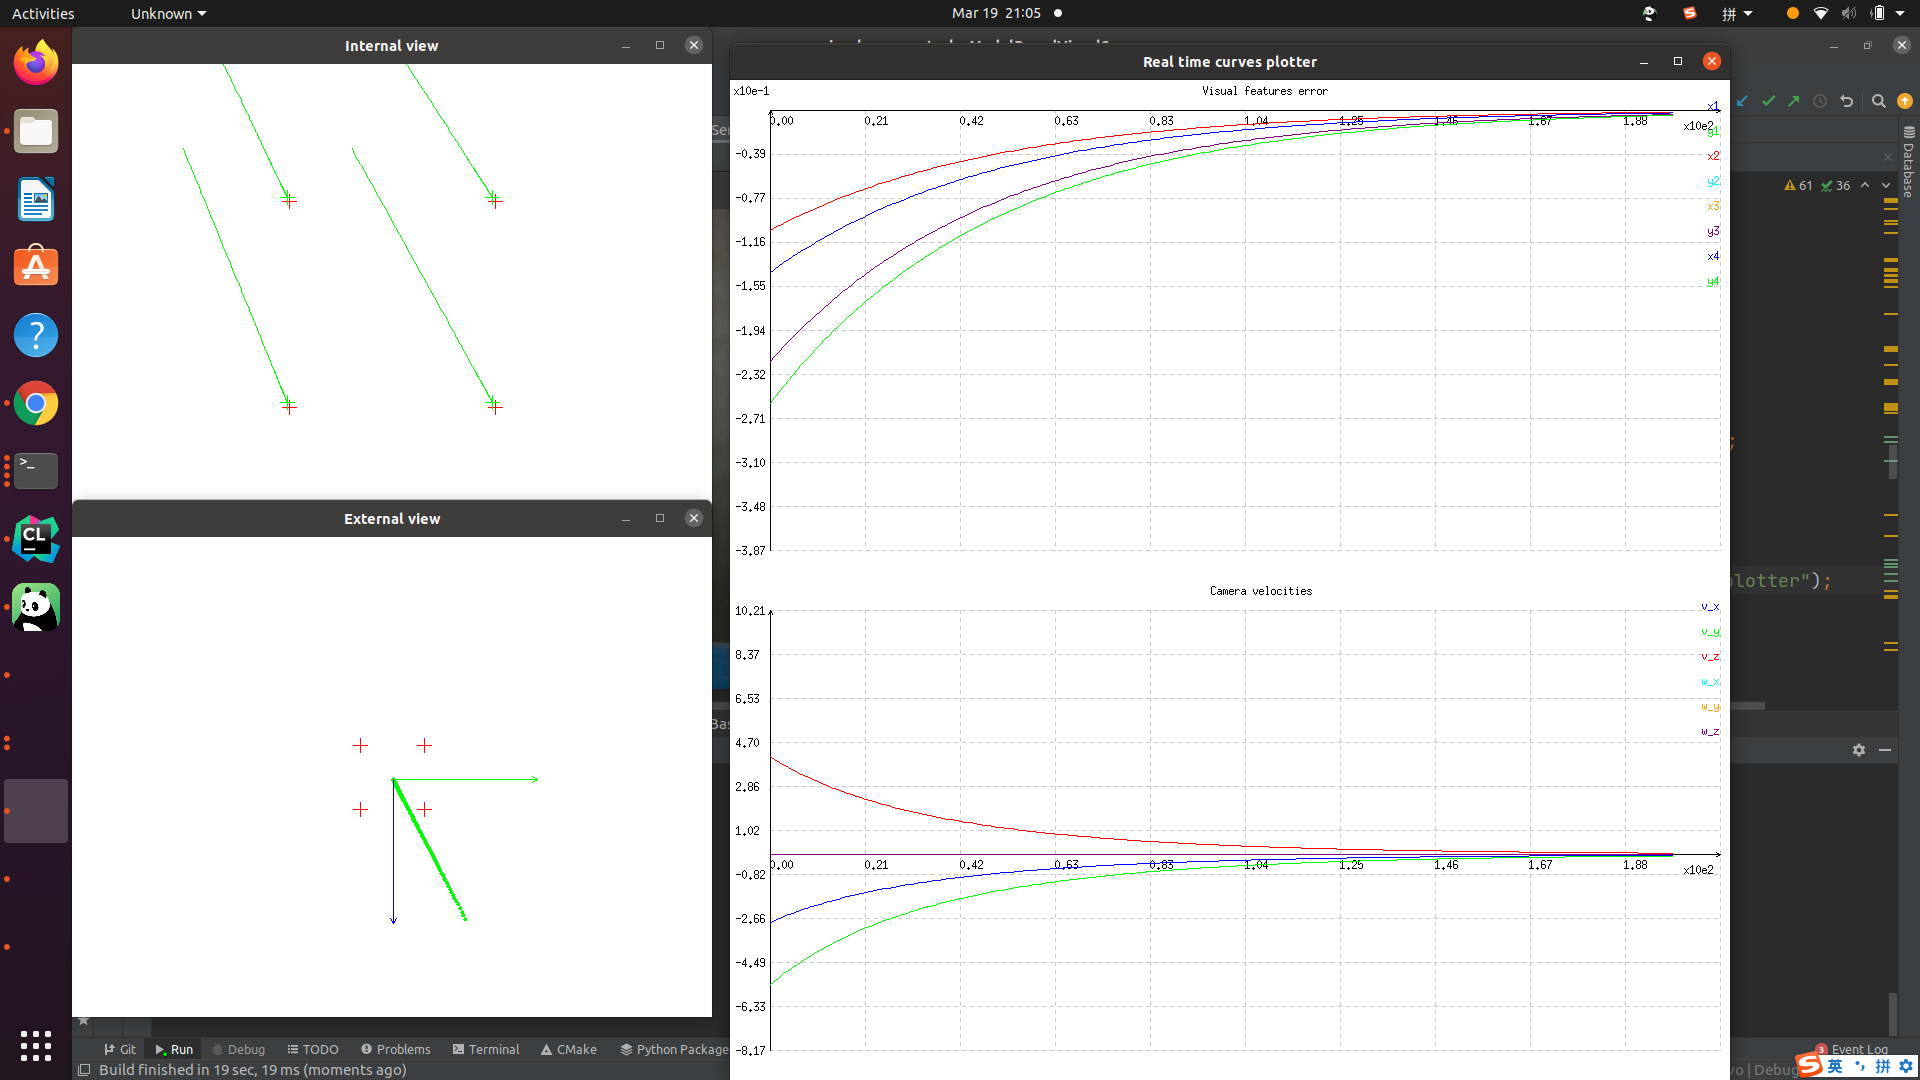
\includegraphics[width = 1.0\textwidth]{chapter2/基于VISP视觉伺服仿真}
\caption{基于VISP视觉伺服仿真}
\label{基于VISP视觉伺服仿真}
\end{figure}


提前在程序中设置好特征的位置,和与之对应的目标特征。将仿真得到的速度指令通过ROS2节点发布订阅机制传输给机器人仿真节点,机器人会相应地运动并使当前特征都到达目标特征处,从而到成到达目标位置处的目的。
\section{IBVS实际系统实现}[Content specification]
\subsection{IBVS实物系统平台搭建}[Content specification]
仿真终归只能用于定性分析。外界干扰、噪声多种多样,仿真中不可能把所有因素考虑进去。事实上,仿真跑出的结果往往十分顺滑,而实物中会反映很多处理不够细节的问题。我认为,IBVS算法在实物上成功运行,研究才算真正的开始。实物运行环境包括JK机器人和装载它并固定它底座的台子;用于承载目标物体的平台和目标;平台上铺盖的一层漫反射效果好且为单一白色的纸;机器人末端装配Realsense D435i深度相机(夹具暂时未装配,在正式夹取的时候会安装在末端)。之所以要铺一层纸,除了保证平面平整且颜色单一以外,还保证了深度相机不要因为丢失反射光导致获取无效数据。最终实物环境图如图\ref{实物环境搭建展示图}所示:
\begin{figure}[h]
\centering
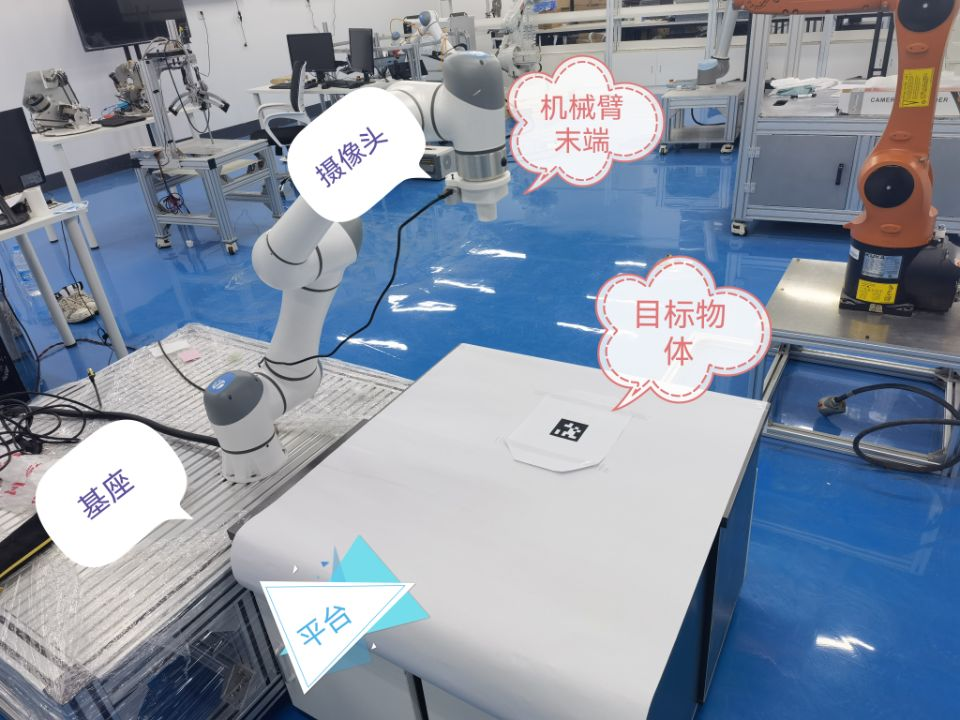
\includegraphics[width = 0.75\textwidth]{chapter2/实物环境搭建展示图}
\caption{实物环境搭建展示图}
\label{实物环境搭建展示图}
\end{figure}

\subsection{IBVS实际运行}[Content specification]
为了能更快地验证IBVS算法,在平台上贴了一张黑色方框码,经过视觉二值化、边缘获取、多边形拟合等处理。实验进行前会将机械臂末端调到目标位置,此时黑色方框会处于摄像头的中央,记录此时的四个点为目标特征。将机器人末端初始位置调至远离黑色方框的位置,距离目标位置的三维各个方向以及Z轴角度都有一定的偏差($\lbrace$\textit{B}$\rbrace$中,$\varDelta X=0.3m,\varDelta Y=0.3m,\varDelta Z=0.5m$)。伺服过程中会不断捕获它的四个点作为特征,并计算特征偏差,最后映射成末端速度指令。伺服的成功证实了所实现的IBVS算法的正确性,同时也正式踏入对未知物体视觉伺服抓取的研究领域中。\ref{视觉伺服曲线绘制(初始)}展示了伺服过程中机械臂末端速度指令和各特征点的偏差对应的曲线。
\begin{figure}[h]
\centering
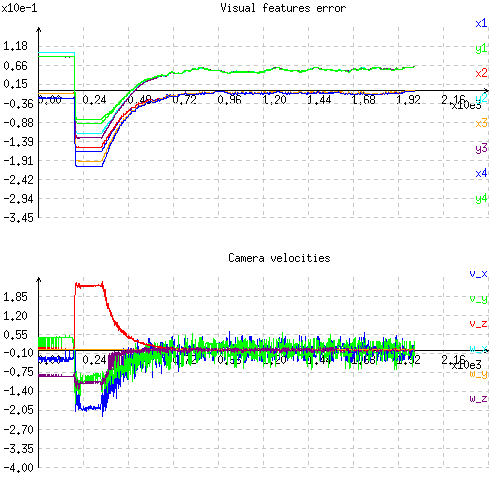
\includegraphics[width = 0.8\textwidth]{chapter2/视觉伺服曲线绘制(初始)}
\caption{视觉伺服曲线绘制(初始)}
\label{视觉伺服曲线绘制(初始)}
\end{figure}
\newpage
\section{本章小结}[Content specification]
本章讲述了基于特征点交互矩阵的IBVS的原理。在算法实现前建立系统坐标系和视觉坐标系,这会使之后的坐标描述便捷许多。搭建了IBVS的仿真运行环境,便于后续问题分析。搭建了实物运行环境,并成功运行了IBVS算法,这意味着研究真正的开始。
%%%%%%%%%%%%%%%%%%%%%%%%%%%抓取目标生成算法研究%%%%%%%%%%%%%%%%%%%%%%%%%%%%
\chapter[伺服目标生成算法研究]{伺服目标自主生成算法研究}
\section{引言}[Content specification]
第二章完成了IBVS的模型建立、仿真系统搭建以及在实物上成功运行IBVS算法,这些为后续的研究提供了控制基础。现在机器人知道自己怎么动了,那么它面对未知物体抓取任务时如何知道自己往哪动呢?接下来,在本章中将对本次课题又一基石——伺服目标生成的研究进行展开。主要研究了基于模型的点云识别和抓取点生成网络两种方法,将它们进行比较后,选择了后者作为应对未知物体抓取任务时生成机器人伺服目标的方案。


\section{基于模型的点云识别与配准}[Content specification]
\subsection{方法陈述}
虽然物体样式多种多样,但它们总以一类一类的形式呈现,例如不同种类的苹果,形状会类似,苹果和球形状类似。对于每一类这样的物体称为一个模型,而对于每一个模型会有一个确定的抓取方式。先收集尽可能多的点云,计算它们的点云特征,对特征类似的进行聚类,计算每一类特征的平均值作为一个模型。每个模型会人为的设定点云中的部分特别位置的点作为期望特征。制作的其中一个圆柱类模型如图\ref{圆柱类点云模型}所示:
\begin{figure}[h]
\centering
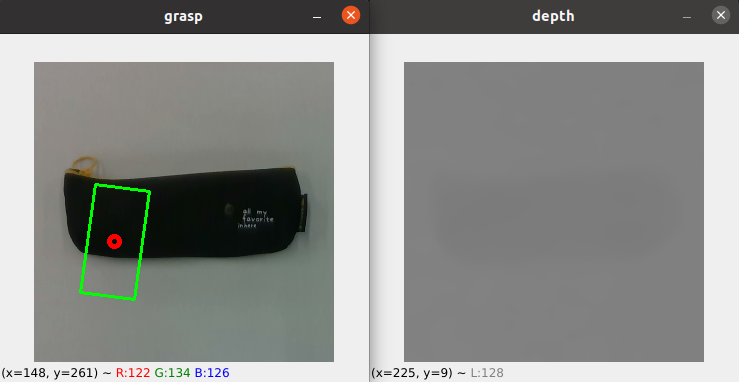
\includegraphics[width = 0.8\textwidth]{chapter3/实时抓取点生成}
\caption{圆柱类点云模型}
\label{圆柱类点云模型}
\end{figure}


对于新来的未知物体,对每个模型进行ICP配准,解算当前物体相对模型的姿态,然后与原模型一致的方式提取当前点云特征,匹配模型的期望特征。将期望特征和提取的特征输入到IBVS控制器中完成伺服控制。


ICP即为迭代最近点法。假设有PA和PB两个点云,它们是相同物体的不同位姿时深度传感器获取的点云。该算法通过不断迭代它们之间的坐标变换矩阵参数的方式让两个点云尽可能的重叠\cite{chetverikov2002trimmed}。设PA和PB的点云分布分别为$p\left( x,y,z \right) $、$q\left( x,y,z \right) $,目前需要找到$P$到$Q$的旋转矩阵$R$和平移矩阵$T$,给出一个代价函数,通过最小二乘法求解最优解。在这之前,先表示出两点云的质心:
\begin{equation}
\left\{ \begin{array}{c}
	\vec{p}=\frac{1}{n}\sum_{i=1}^N{\vec{p}_i}\\
	\vec{q}=\frac{1}{n}\sum_{i=1}^N{\vec{q}_i}\\
\end{array} \right. 
\label{点云质心描述1} 
\end{equation}


然后从两个点集中的每个点减去相应的质心:
\begin{equation}
\left\{ \begin{array}{c}
	\vec{p}_t=\vec{p}_i-\vec{p}\\
	\vec{q}_t=\vec{q}_i-\vec{q}\\
\end{array} \right. 
\label{点云质心描述2} 
\end{equation}


则上述最优化目标函数可以转化为:
\begin{equation}
E=\sum_{i=1}^N{\left| \vec{q}_t-R\vec{p}_t \right|}
\label{ICP代价函数} 
\end{equation}


最优化问题最后分解为:
\begin{itemize}
\item[(1)]
求使代价函数$E$最小的旋转矩阵$R$。
\item[(2)]
求得平移矩阵$T=\vec{q}-R\vec{p}$.
\end{itemize}

\subsection{算法实现}
深度传感器获得的点云往往不全是目标物体的点云,在姿态匹配前,经过三个方向的点云截断滤波、去离群点、降采样操作,最后提取出目标点云。基于模板匹配点云识别过程中所提取的点云特征选取了VFH特征,它是一种全局特征,可以快速计算和匹配。算法的实现效果如图\ref{基于模型的点云识别实操图}和图\ref{基于模型的点云识别效果图}所示。


图\ref{基于模型的点云识别实操图}和图\ref{基于模型的点云识别效果图}分别是算法运行时第三方视角和电脑视角的图片,点云处理间隔为500ms,但识别和位姿解算间隔约为3s。
\newpage
\begin{figure}[h]
\centering
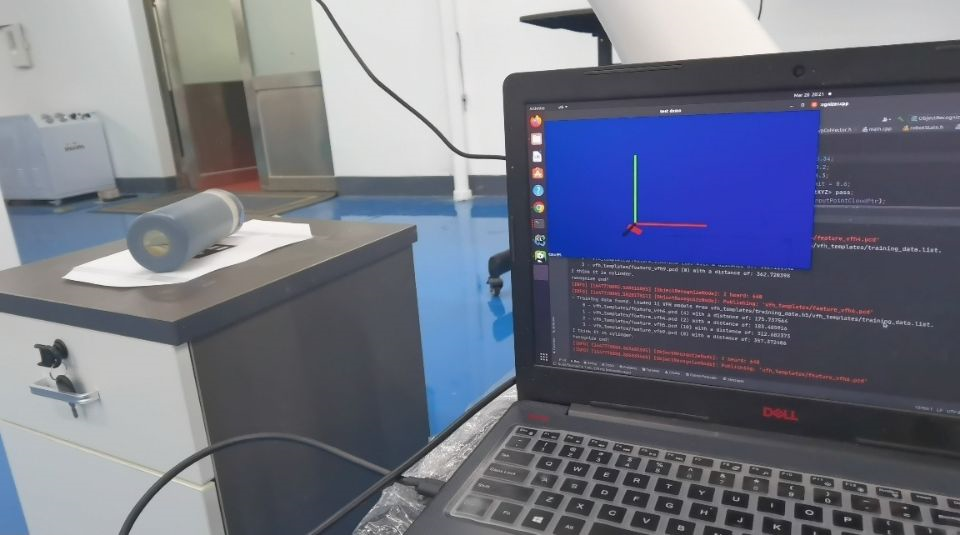
\includegraphics[width = 0.75\textwidth]{chapter3/基于模型的点云识别实操图}
\caption{基于模型的点云识别实操图}
\label{基于模型的点云识别实操图}
\end{figure}

\begin{figure}[h]
\centering
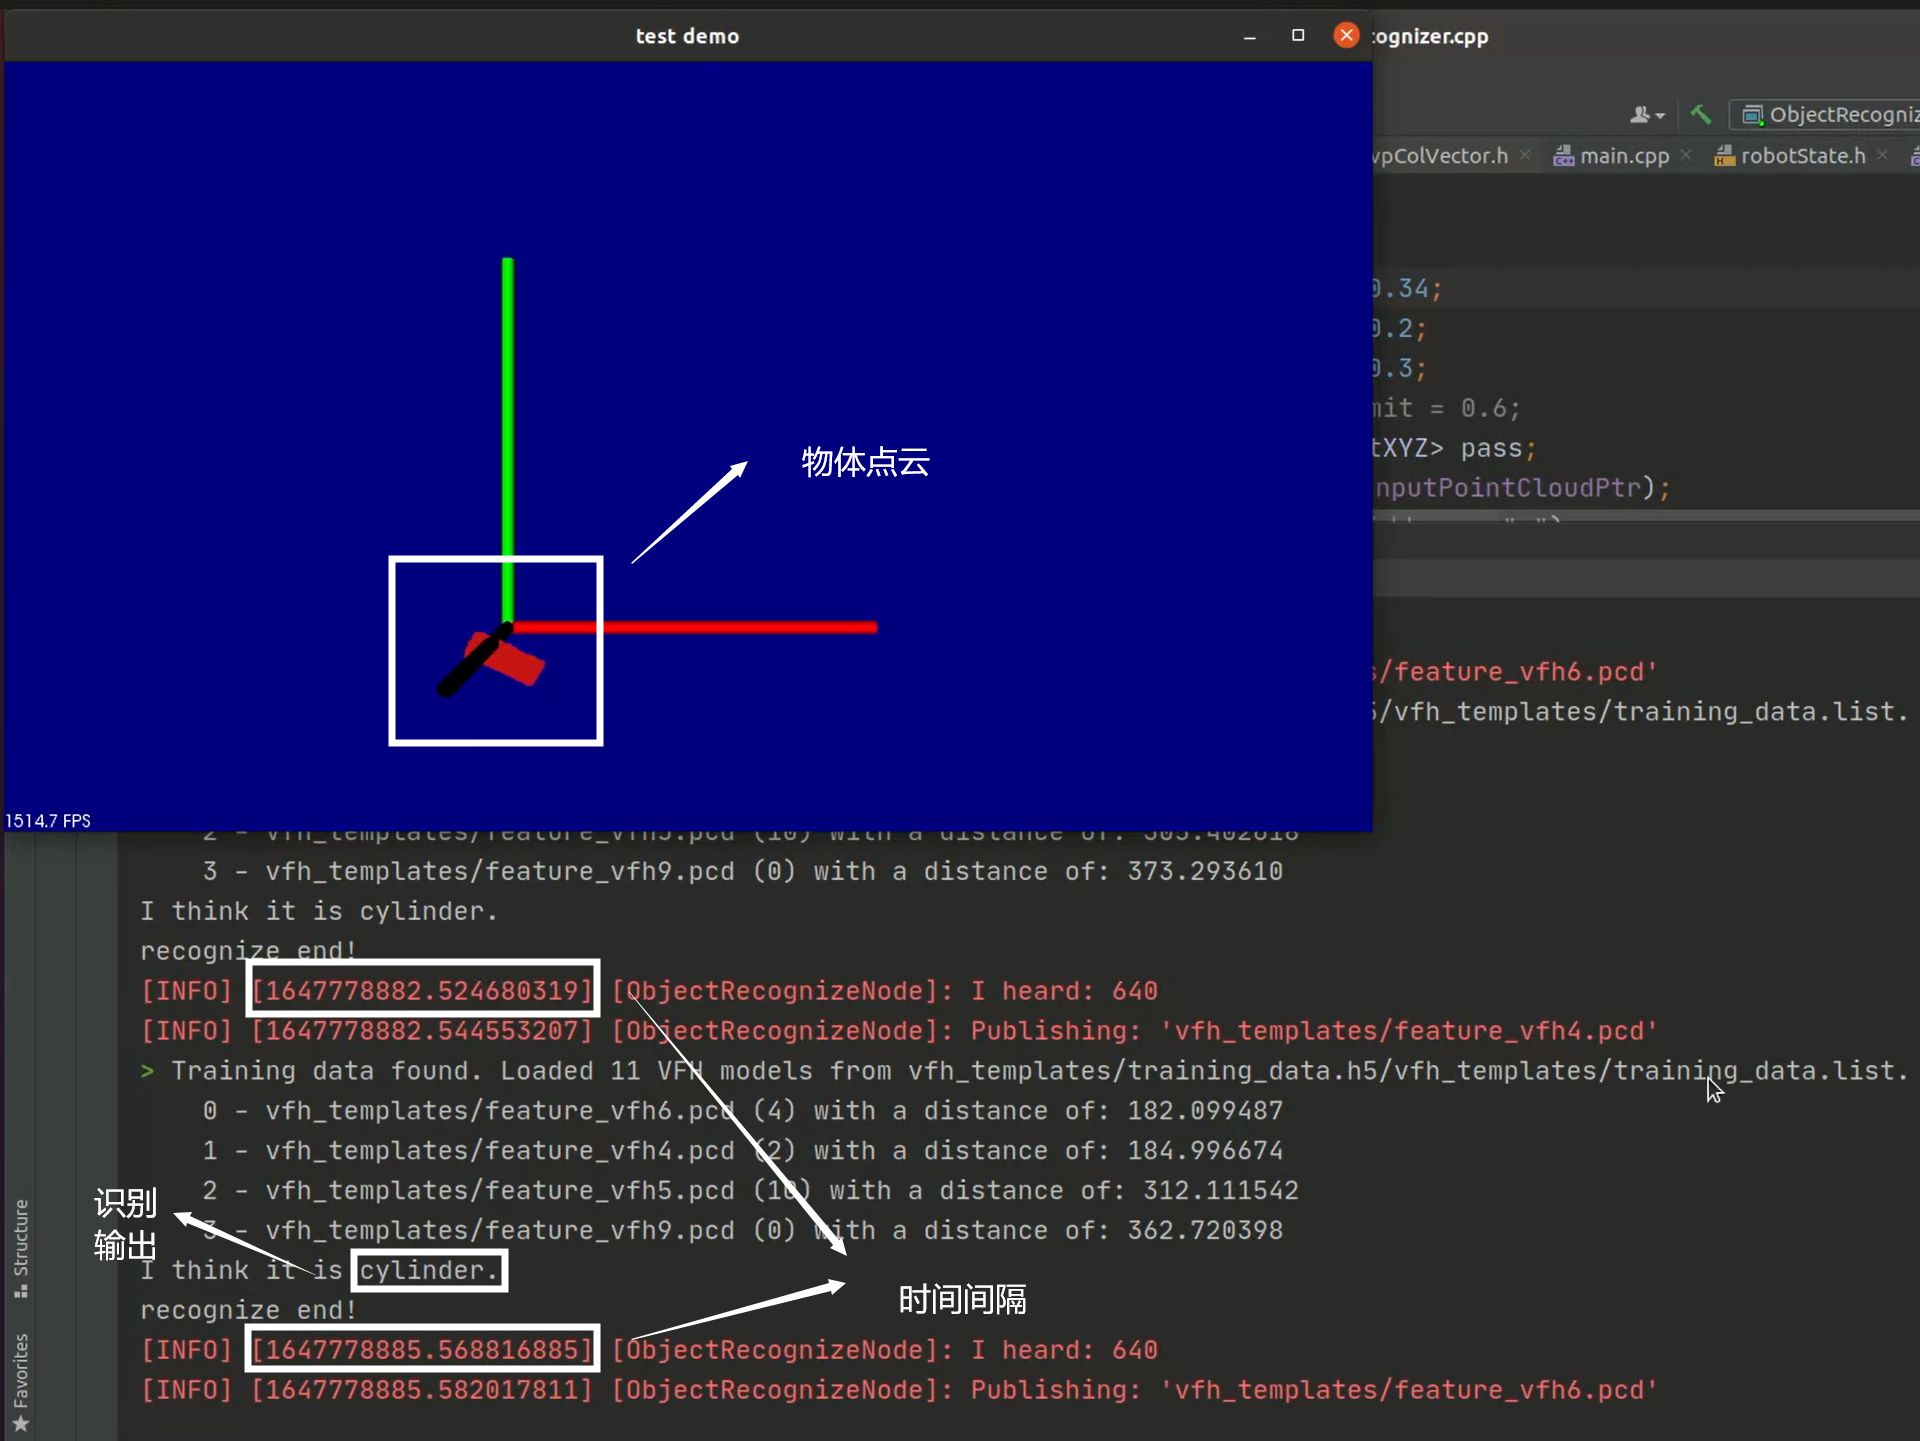
\includegraphics[width = 0.75\textwidth]{chapter3/基于模型的点云识别效果图}
\caption{基于模型的点云识别效果图}
\label{基于模型的点云识别效果图}
\end{figure}
\subsection{方法小结}
该方法需要环境噪声较小时,才能正常匹配,消耗时间长,拖长了系统抓取物体所需运行的时间,且不可用于实时的目标特征生成,视觉伺服效果将会非常依赖初始的视觉、点云处理。另外,还存在模型制作困难、鲁棒性差等问题,这写让这个方法面对卷积神经网络完全没有一战之力。


\section{抓取点生成网络(GG-CNN)}[Content specification]
\subsection{方法陈述}
抓取点生成网络(GG-CNN)属于Grasp Synthesis中的一种,为PBVS量身订做的抓取点生成方案。Douglas Morrison等人在2018年提出了GG-CNN,该网络非常轻便快捷,可以通过输入深度图像,在19ms内输出图像中机器人的期望抓取位姿,最后依赖相机内参、外参计算出机械臂末端期望的位姿,通过PBVS来抓取未知物体\cite{morrison2018closing}。该工作最大的特点是,它能让视觉伺服实时生成期望位姿,伺服精度不再受初始计算的期望位姿影响。在后续研究中,会通过一个很特别而简单的方法将该网络所输出的结果应用于IBVS,但在这之前,先要弄清楚它的工作原理。


他们创新性在于提出了十分合适的网络输出。网络整体结构的设计是非常简单的,追求大感受野,然后就是很寻常的叠层。网络限定了机器人末端需要时二指的,视觉伺服控制中,相机必须保持时刻俯视,这也是在第二章实物搭建中这么做的原因之一。网络的本质是语义分割,输出4张与输入的300*300深度图像相同大小的图像$G=\left[ Q,W,\varPhi \left( \sin \theta ,\cos \theta \right) \right]$,其中使用$\sin \theta$和$\cos \theta$分别对应不同的输出图片。$Q$图像中每个像素代表这个点的抓取质量,它们都是被归一化的数据,1表示抓取质量很高,0表示这个点完全不值得抓取;$W$图像中每个像素代表抓取这个点所需要的二指张开宽度;$\varPhi$图像中每个像素代表抓取这个点所需要的二指沿Z轴旋转角度。


本文中认为他们所构建的网络有很大的优化空间。他们为了加快网络计算速度,所设计的层数太少,网络的非线性程度较低。所以使用1*1卷积层对网络非线性化。其次,作者非常喜欢使用大卷积核。实际上在机械臂末端运动过程中,物体在相机中的大小会有很大的改变,单一感受野并不能适应这样的变化,所以将大卷积核拆成不同尺度小卷积核的叠加。以上的优化并不会带来太多的计算量,因为改动的地方只是增加了1*1卷积层和拓展的小卷积核,它们本身不会带来什么计算量。最终网络如图\ref{GG-CNN改进}所示。
\begin{figure}[h]
\centering
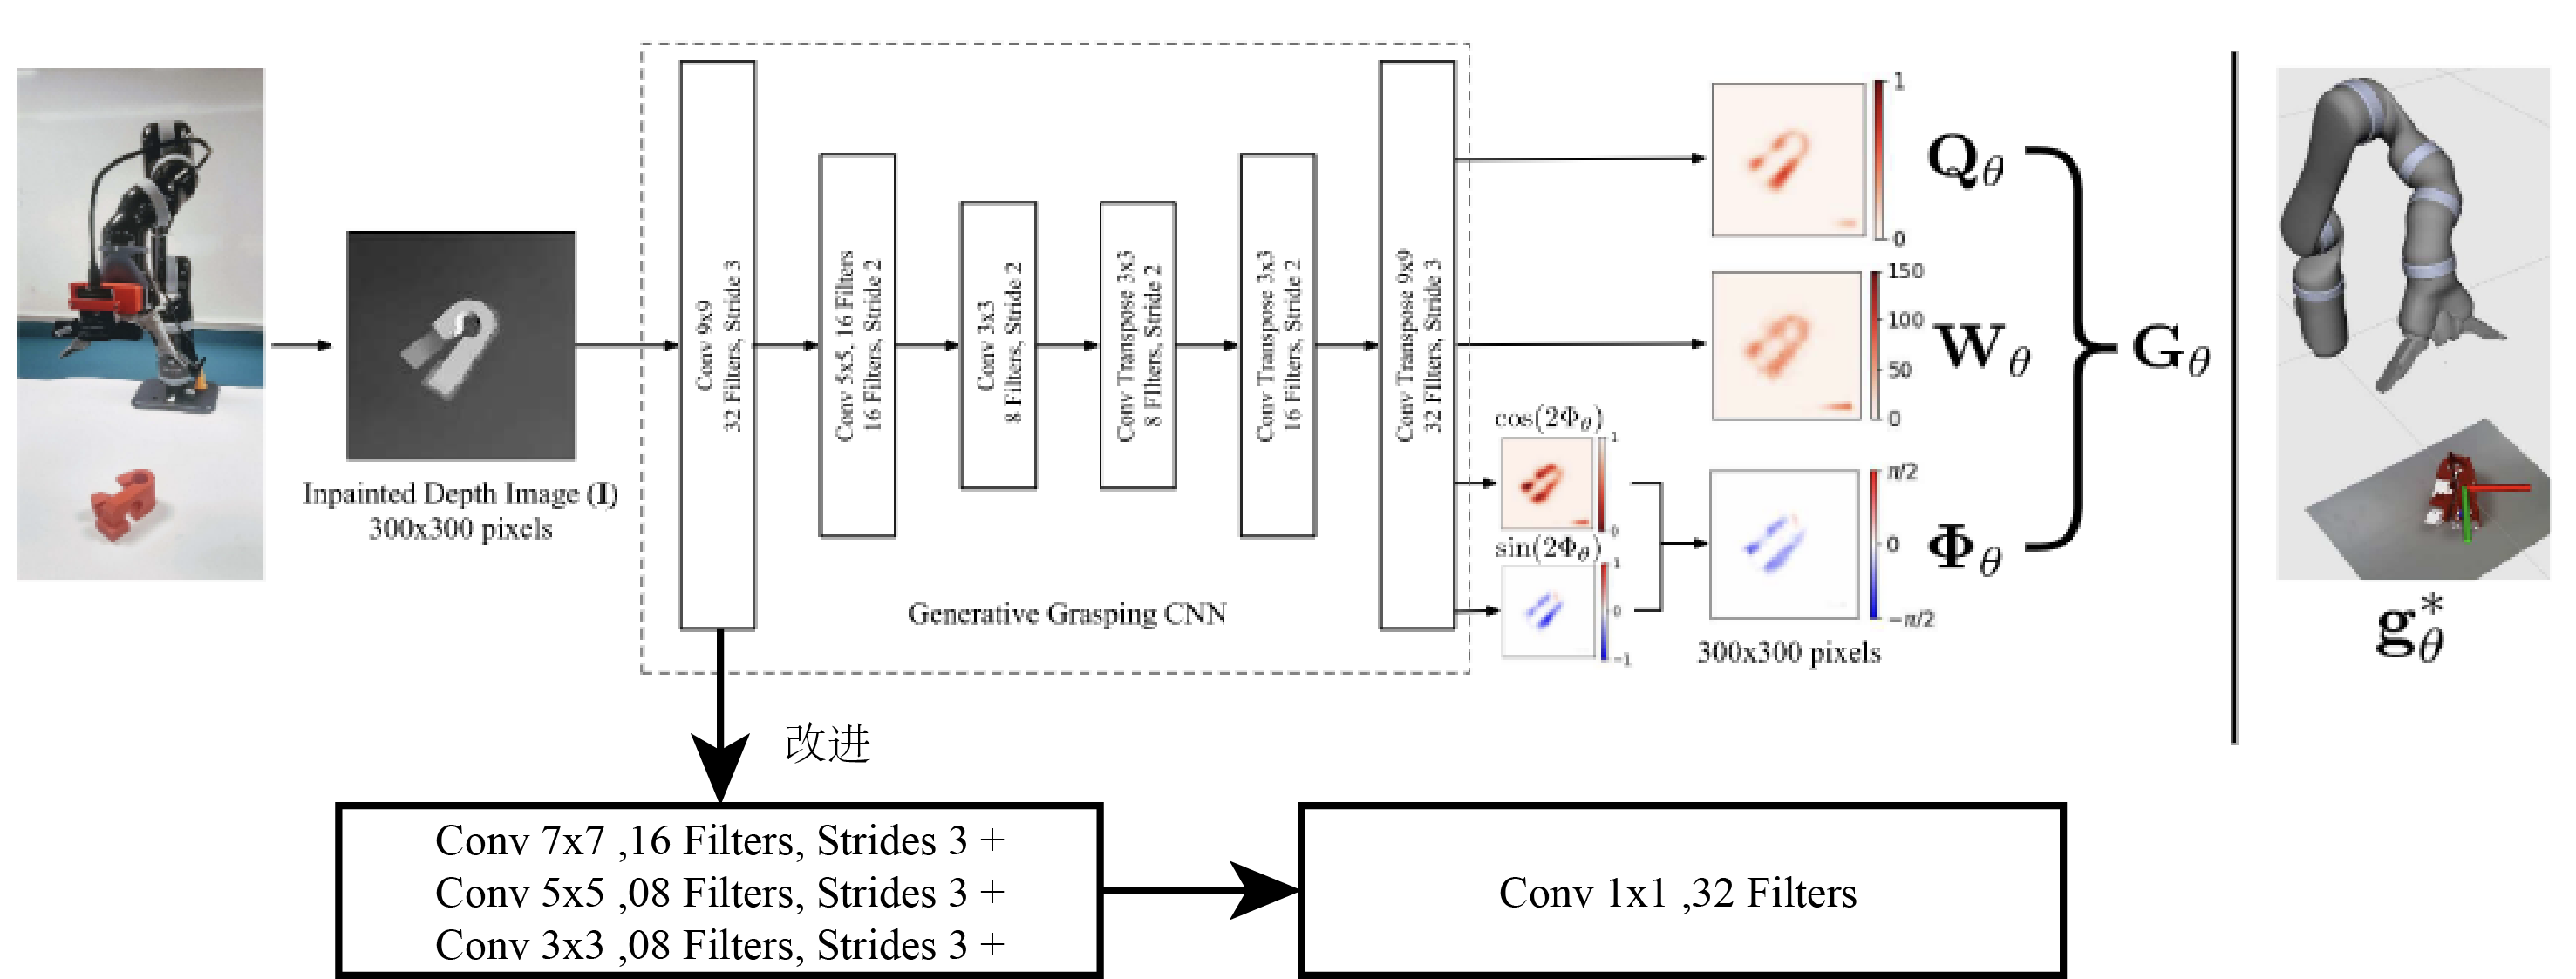
\includegraphics[width = 1.0\textwidth]{chapter3/GG-CNN改进}
\caption{GG-CNN改进后网络架构}
\label{GG-CNN改进}
\end{figure}


\subsection{算法实现}
配好pytorch环境,使用Cornnel数据集。将计算出的最大抓取质量像素点作为长方形中心,$\varPhi$为长方形绕中心旋转角度,$W$作为长方形的长,长方形宽为它的1/2,绘制长方形框,将计算出的IoU(预测抓取框与标签抓取框对应交集与并集的比)作为预测准确率,选取数据的10\%作为测试集,跑通优化后的GG-CNN代码训练程序,约40 epoch时达到了对测试集的80\%准确率。这个准确率相对于原始程序上升了4\%,优化是有效的。对给定深度图,输出效果如图\ref{GG-CNN输出(初始)}所示:
\begin{figure}[h]
\centering
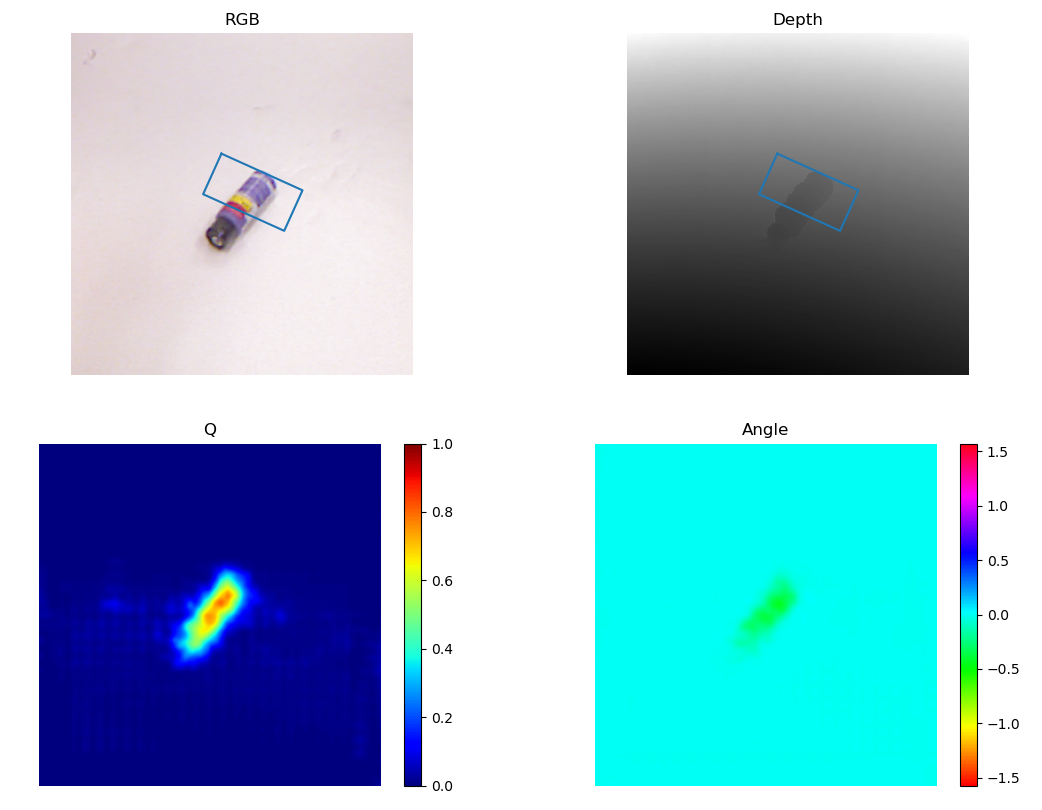
\includegraphics[width = 0.75\textwidth]{chapter3/GG-CNN输出(初始)}
\caption{GG-CNN输出}
\label{GG-CNN输出(初始)}
\end{figure}


这里特别解释一下图\ref{GG-CNN输出(初始)}中图Q表示抓取质量热度图,颜色越偏暖色越值得被抓,图Angle表示抓取角度图,单位是弧度,可以看到对柱形物体,抓取角度在高抓取质量点处几乎一致。


在代码测试过程中发现Realsense D435i对深度的测量信噪比很低,测量深度波动很大,只依靠深度图像一阶图像矩无法稳定定位目标物体的位置,所以通过RGB图像和深度图像的一阶图像矩(如果能有更好的深度传感器,是不需要依赖颜色信息的)可以得到目标大致位置。使用这个作为中心对当前640*480的图像进行考虑边缘(如果超出原始图像范围,会平移中心)的300*300裁剪。将神经网络写成ROS2的一个节点,实时发布计算出的抓取点信息,视觉伺服节点会订阅它的主题,实时显示抓取方框。选择抓取对象为笔袋,图\ref{实时抓取点生成}为实时抓取点生成效果图。
\begin{figure}[h]
\centering
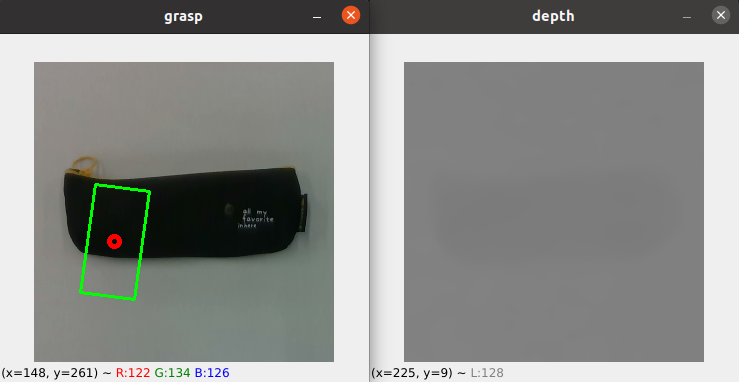
\includegraphics[width = 0.75\textwidth]{chapter3/实时抓取点生成}
\caption{实时抓取点生成}
\label{实时抓取点生成}
\end{figure}


实时显示抓取框和之前只显示一次抓取框有很大的不同,因为神经网络输出的抓取质量在目标位置处会有很多相近的点,如果物体具有平移对称性或者旋转对称性,抓取点的位置会不断跳动,正如图\ref{神经网络原始输出}所示。这会使生成的目标特征不断摆动,导致系统失稳。(由于角度为弧度制过太小,输出时乘了100倍)
\begin{figure}[h]
\centering
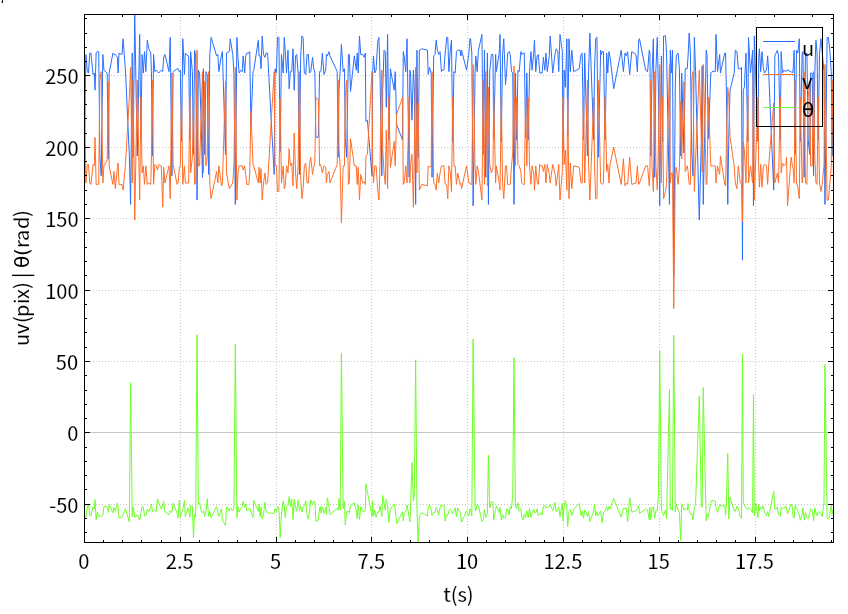
\includegraphics[width = 0.75\textwidth]{chapter3/神经网络原始输出}
\caption{神经网络原始输出}
\label{神经网络原始输出}
\end{figure}


在GG-CNN原文中给出的解决方式是计算抓取质量图中三个局部最大点,选择与上一次的抓取点最近的点作为本次的抓取点。但是研究中在复现他们的算法后依然无法解决波动很大的问题,甚至调高选择的局部最大点个数到10。本文认为这是物体平移、旋转对称性带来的必然结果,无论网络好坏,因为网络的输入是深度图像。所以该网络输出的抓取点位置信息无法使用,只能委曲求全使用RGB图像的一阶图像矩代替,毕竟在裁剪图像的时候就求取过一阶图像矩的值。颜色信息在所搭建的实验环境中是非常稳定的,这样稳定的抓取点中心可以被用于实时抓取点生成。只是使用该方法会带来另一个麻烦,在伺服末期,如果目标靠近平台边缘,摄像头将捕捉地面的颜色信息,会对抓取点中心的计算带来干扰,这个问题将在本文第四章和其它问题一并解决。


好在角度的波动能得到很好的解决。因为相机时刻俯视向下,所以相机期望的沿Z轴的旋转角度和抓取框旋转角度是一致的。对于这样一个线性系统,使用卡尔曼滤波可以有效抑制噪声。机械臂末端沿Z轴的角速度设为$\omega_z$,它由每次控制周期$\delta _t$的IBVS控制器计算出。机械臂末端旋转角度为$\theta_z$,可以通过读取机械臂编码器的值间接获取。可以写出状态、观测方程:
\begin{equation}
\hat{x}_{k+1}=\left[ \begin{array}{c}
	\theta _z\\
	\omega _z\\
\end{array} \right] _{k+1}=\left[ \begin{matrix}
	1&		0\\
	0&		\delta _t\\
\end{matrix} \right] \left[ \begin{array}{c}
	\theta _z\\
	\omega _z\\
\end{array} \right] _k=A\hat{x}_k
\label{状态方程}
\end{equation}
\begin{equation}
z_{k+1}=\theta _z=\left[ \begin{matrix}
	1&		0\\
\end{matrix} \right] \left[ \begin{array}{c}
	\theta _z\\
	\omega _z\\
\end{array} \right] _k=H\hat{x}_k
\label{观测方程}
\end{equation}


认为过程噪声$\omega_k$和观测噪声$\upsilon_k$都服从高斯分布:
\begin{equation}
\left\{ \begin{array}{c}
	p\left( \omega \right) \sim N\left( 0,Q \right)\\
	p\left( \upsilon \right) \sim N\left( 0,R \right)\\
\end{array} \right. 
\label{噪声分布}
\end{equation}


则有协方差矩阵的预测方程:
\begin{equation}
\hat{P}_{k+1}=AP_kA^T+Q
\label{协方差预测}
\end{equation}


设卡尔曼滤波的增益为$K$,则根据以上条件求得:
\begin{equation}
K_{k+1}=\hat{P}_{k+1}H^T\left( H\hat{P}_{k+1}H^T+R \right) ^{-1}
\label{卡尔曼滤波的增益}
\end{equation}


使用观测器数据对当前预测状态进行更新,对卡尔曼滤波器的初始化中,令$R$、$Q$都为单位矩阵:
\begin{equation}
x_{k+1}=\hat{x}_{k+1}+K_{k+1}\left( z_{k+1}-H\hat{x}_{k+1} \right) 
\label{卡尔曼滤波的增益}
\end{equation}


再使用新的预测的状态更新协方差矩阵:
\begin{equation}
P_{k+1}=\left( I-K_{k+1}H \right) \hat{P}_{k+1}
\label{更新协方差矩阵}
\end{equation}


在机械臂静止不动时,神经网络预测的抓取点中心、角度随时间变化曲线如图\ref{抓取点中心方法替代与角度滤波}所示。得到的抓取中心只有1到2像素点的波动,预测的抓取角度几乎不再波动。
\begin{figure}[h]
\centering
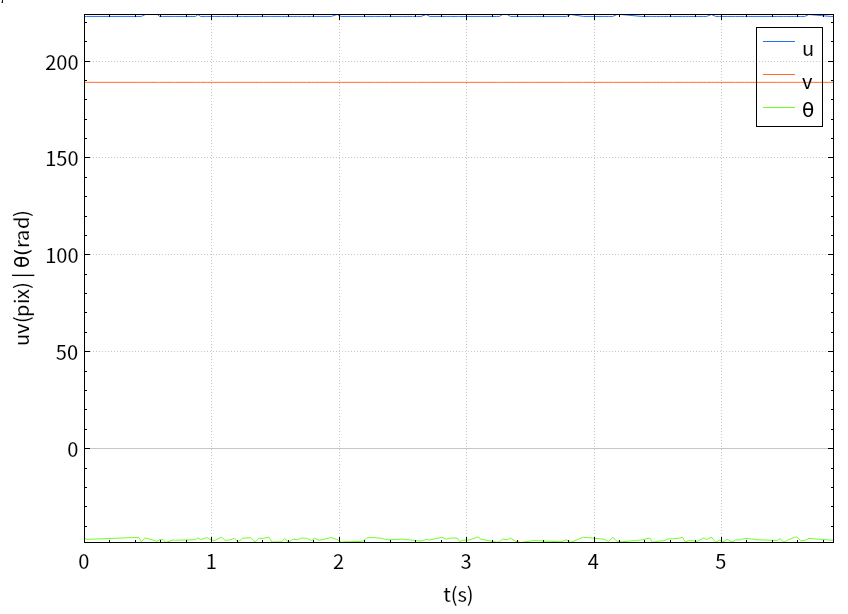
\includegraphics[width = 0.75\textwidth]{chapter3/抓取点中心方法替代与角度滤波}
\caption{抓取点中心方法替代与角度滤波}
\label{抓取点中心方法替代与角度滤波}
\end{figure}

\subsection{方法小结}
GG-CNN是十分契合本次研究目的的研究成果,因此它被选作未知物体抓取算法中解决机械臂怎么去抓取目标的方法。但是在复现工作中遇到了抓取中心波动过大的无法解决的问题,只能使用RGB图像的一阶图像矩方法代替它进行抓取点中心生成,最终只保留了该网络输出的角度项,在经过卡尔曼滤波处理后拥有比较稳定的输出值。

\section{本章小结}[Content specification]
本章研究了两种伺服目标自主生成的算法,比较后,选择了后者作为后续研究生成伺服目标的主要方法。相比于传统的基于模型获取抓取点的方法,神经网络有更好的鲁棒性、实时性。但是目前选取的GG-CNN并不是完美的,在实时伺服中它的抓取点中心因为目标物体平移、旋转对称性的存在,波动大到无法使用滤波的方法来抑制了。所以使用RGB一阶图像矩来生成抓取点中心。对于网络输出的抓取角度使用线性卡尔曼滤波对波动进行有效的抑制。


%%%%%%%%%%%%%%%%%%基于GG-CNN和IBVS的未知物体抓取算法实现%%%%%%%%%%%%%%%%%%%
\chapter[未知物体抓取算法实现]{未知物体抓取算法实现}
\section{引言}[Content specification]


\section{机器人视觉伺服系统概述}[Content specification]



%%%%%%%%%%%%%%%%%%%%%%%%%%%%%IBVS控制律优化%%%%%%%%%%%%%%%%%%%%%%%%%%%%%%
\chapter[IBVS控制律优化]{IBVS控制律优化}
%%%%%%%%%%%%%%%%%%%%%%%%%%%%%实验设计与验证%%%%%%%%%%%%%%%%%%%%%%%%%%%%%%
\chapter{实验设计与验证}
\section{引言}[Content specification]
前面的章节中详细说明了通过视觉伺服抓取未知物体的思路、视觉伺服控制律的优化以及它们的实现过程。在前人的研究成果基础上,这套未知物体抓取算法提出创新性的特征点提取、匹配方式和与之配套的视觉伺服控制律。它将在更少的环境条件限制下拥有更高的未知物体抓取率和更理想平滑的曲线。本章将对一共八个家常物体,每个物体八种位姿进行抓取实验,然后将抓取成功率与各生成抓取合成类方法进行比较,证明这套未知物体抓取算法的优越性。另外,会对不同物体同一位姿、相同物体不同位姿的伺服曲线进行记录,通过超调、响应时间等参数反映算法应对多种多样情况下的高鲁棒性。

\section{实验设计}[Content specification]
对于未知物体抓取任务,抓取成功率是最需要关注的指标。为了使成功率的测试结果能体现系统应对各种情形下的抓取能力,需要实验中的抓取目标种类多样化和位姿多样化。另外,为了能与提出GG-CNN原文献抓取成功率结果相对公平性的横向比较,尽量搭建相同的实验环境和使用相同的抓取目标。


根据算法的实现过程,实验过程中存在的限制条件如下:
\begin{itemize}
\item[(1)]
由于研究中GG-CNN对输入深度图像的尺寸需求和清晰度需求,需要对目标的进行范围裁剪,这时会使用RGB信息确定目标的中心大致范围,所以实验中在平台上铺盖的白纸是必须的。如果有更好的网络能不需要裁剪并稳定指出目标位置,实验环境中白色背景的条件可以被去除。
\item[(2)]
GG-CNN的输出形式决定了如果要使用它的输出结果作为视觉伺服的依据,必须保证相机时刻俯视0°朝下,所以对末端的沿X、Y轴角速度指令不论计算结果如何都会在给机械臂下达命令那一步置零。
\item[(3)]
深度传感器使用的Realsense D435i,它是基于结构光的原理测量深度的,所以对漫反射能力差的目标,获取的深度值几乎是无效值,所以选用的目标都是漫反射效果好的物体。另外,它的深度测量精度为1mm,这决定了选用目标不可以是铅笔等过小的物体,当然,也不可以过大,这会让神经网络无法区分谁是目标谁是背景。
\end{itemize}


实物环境搭建如图\ref{实物环境搭建展示图},这与GG-CNN原文是类似的。但值得一提的是,经过第四章中对RGB图像和深度图像的特别处理,本文中机械臂的运动范围可以超出平台范围(但初始情况时,目标必须在相机视野范围内),这是相对GG-CNN原文具有优势的地方。根据限制条件(3)和仿照GG-CNN原文使用的抓取目标,选择了八种家常抓取目标用于本次实验的各种测试与验证,它们是什么{\color{red}正如图所示}:


抓取目标将以对称的姿态在平台的八个方位的位置摆放,这么做可以很全面地测试伺服系统应对多样化的目标位姿的伺服情况,摆放示意图{\color{red}如图?所示}:


{\color{red}六轴JK机械臂初始状态各编码器显示数值为:机械臂末端在$\lbrace$\textit{B}$\rbrace$中的初始状态为:。在这样的初始参数设计下,摄像头获取的图片如图?所示,正好可以将整个平台尽收眼底。
相对机械臂末端,目标摆放位置和对应姿态如表?所示}


实验中将会在八种不同的物体的八种不同位姿情况下对目标进行抓取,记录的实验结果包括是否成功抓取,伺服超调量和响应时间。响应时间不包括抓物体所需时间,因为抓取是开环控制的,所需时间固定,没有记录的必要。开环抓取效果在第四章有详细介绍。然后会与各个基于生成抓取合成方法来抓取未知物体的文献成果进行比较。最后对不同物体相同位姿以及抓取率百分之百的一个物体不同位姿伺服曲线进行分析,并与同样基于GG-CNN但使用PBVS+IBVS来抓取未知物体的文献成果\cite{haviland2020control}进行比较。
\section{人机交互界面设计}[Content specification]


\section{实验验证}[Content specification]
\subsection{抓取成功率测试}[Content specification]
对总共64种情况的实验结果进行记录,不仅记录总的抓取成功率,同时记录相同物体的抓取成功率和相同位姿对应不同物体的抓取成功率,绘制表格如下:


通过该表格展现的数据,反应所提出的未知物体抓取算法特点如下:


将实验获得的数据与各类成抓取合成方法的文献成果在一张表格中进行展现:


表格反映了。。。
\subsection{抓取性能验证}[Content specification]
选择的目标为。。。,把它不同的摆放位姿情况下的特征偏差曲线绘制到同一坐标系下,将不同情况对应的超调量和响应时间绘制到直方图中,如图?所示:


从图?中可以看出。。。


选择的位姿为。。。,把对应的不同目标情况下的特征偏差曲线绘制到同一坐标系下,将不同情况对应的超调量和响应时间绘制到直方图中,如图?所示:


图?为同样基于GG-CNN但使用PBVS+IBVS来抓取未知物体的伺服过程中特征偏差曲线,他还测量了运动物体的伺服情况,相关曲线忽略。比较静止物体的伺服情况,有以下结论。。。
\section{本章小结}[Content specification]
本章在八种不同家常的物体的八种不同位姿情况下对目标进行抓取实验,在所提出的特征提取、匹配的方法和与之配套的伺服控制律的加持下,在环境限制条件更少的情况下,拥有比许多类似工作的研究成果更高的抓取成功率。与另一个基于GG-CNN抓取未知目标文献成果比较,拥有更平滑而理想的伺服曲线。通过以上实验证明了本研究所提出的未知物体抓取算法有高鲁棒性和高伺服性能。
%% !Mode:: "TeX:UTF-8"

\chapter{示例文档}[Example]

这是 \hithesis\ 的示例文档,基本上覆盖了模板中所有格式的设置。建议大家在使用模
板之前,除了阅读《\hithesis\:哈尔滨工业大学学位论文模板》\footnote{即
hithesis.pdf文件},本示例文档也最好能看一看。此示例文档尽量使用到所有的排版格式
,然而对于一些不在我工规范中规定的文档,理论上是由用户自由发挥,这里不给出样例
。需要另行载入的宏包和自定义命令在文件`hithesis.sty'中有示例,这里不列举。

\section{关于数字}[Number]

按《关于出版物上数字用法的试行规定哈哈哈》(1987年1月1日国家语言文字工作委员会等7个单位公布),除习惯用中文数字表示的以外,一般数字均用阿拉伯数字。
(1)公历的世纪、年代、年、月、日和时刻一律用阿拉伯数字,如20世纪,80年代,4时3刻等。年号要用四位数,如1989年,不能用89年。
(2)记数与计算(含正负整数、分数、小数、百分比、约数等)一律用阿拉伯数字,如3/4,4.5%,10个月,500多种等。
(3)一个数值的书写形式要照顾到上下文。不是出现在一组表示科学计量和具有统计意义数字中的一位数可以用汉字,如一个人,六条意见。星期几一律用汉字,如星期六。邻近两个数字并列连用,表示概数,应该用汉字数字,数字间不用顿号隔开,如三五天,七八十种,四十五六岁,一千七八百元等。
(4)数字作为词素构成定型的词、词组、惯用语、缩略语等应当使用汉字。如二倍体,三叶虫,第三世界,“七五”规划,相差十万八千里等。
(5)5位以上的数字,尾数零多的,可改写为以万、亿为单位的数。一般情况下不得以十、百、千、十万、百万、千万、十亿、百亿、千亿作为单位。如~\num{345000000}~公里可改写为3.45亿公里或~\num{34500}~万公里,但不能写为3亿~\num{4500}~万公里或3亿4千5百万公里。
(6)数字的书写不必每格一个数码,一般每两数码占一格,数字间分节不用分位号“,”,凡4位或4位以上的数都从个位起每3位数空半个数码(1/4汉字)。“\num{3000000}”,不要写成“3,000,000”,小数点后的数从小数点起向右按每三位一组分节。一个用阿拉伯数字书写的多位数不能从数字中间转行。
(7)数量的增加或减少要注意下列用词的概念:1)增加为(或增加到)过去的二倍,即过去为一,现在为二;2)增加(或增加了)二倍,即过去为一,现在为三;3)超额80%,即定额为100,现在为180;4)降低到80%,即过去为100,现在为80;5)降低(或降低了)80%,即原来为100,现在为20;6)为原数的1/4,即原数为4,现在为1,或原数为1,现在为0.25。
应特别注意在表达数字减小时,不宜用倍数,而应采用分数。如减少为原来的1/2,1/3等。


\section{索引示例}[Index]

为便于检索文中内容,可编制索引置于论文之后(根据需要决定是否设置)。索引以论文中
的专业词语为检索线索,指出其相关内容的所在页码。索引用中、英两种文字书写,中文在
前。\sindex[china]{qi!乔峰}\sindex[english]{Xu Zhu}\sindex[english]{Qiao Feng}
中文按各词汉语拼音第一个字母排序,英文按该词第一个英文字母排序。

\section{术语排版举例}[Glossaries and index]

术语的定义和使用可以结合索引,灵活使用。
例如,\gtssbp 是一种应用于狄利克雷过程抽样的算法。
下次出现将是另一种格式:\gtssbp 。
还可以切换单复数例如:\gscnas ,下次出现为:\gscnas 。
此处体现了\LaTeX\ 格式内容分离的优势。

\section{引用}[Cite]

\sindex[china]{du!段誉}引文标注遵照GB/T7714-2005,采用顺序编码制。正文中引用文献的标示应置于所引内容最后一个字的右上角,所引文献编号用阿拉伯数字置于方括号“[ ]”中,用小4号字体的上角标。要求:

(1)引用单篇文献时,如“二次铣削\cite{cnproceed}”。

(2)同一处引用多篇文献时,各篇文献的序号在方括号内全部列出,各序号间用“,”,如
遇连续序号,可标注讫序号。如,…形成了多种数学模型\cite{cnarticle,cnproceed}…
注意此处添加\cs{inlinecite}中文空格\inlinecite{cnarticle,cnproceed},可以在cfg文件中修改空格类型。

(3)多次引用同一文献时,在文献序号的“[ ]”后标注引文页码。如,…间质细胞CAMP含量
测定\cite[100-197]{cnarticle}…。…含量测定方法规定
\cite[92]{cnarticle}…。

(4)当提及的参考文献为文中直接说明时,则用小4号字与正文排齐,如“由文献\inlinecite{hithesis2017}可知”

\section{定理和定义等}[Theorem]
\begin{theorem}[\cite{cnproceed}]
宇宙大爆炸是一种爆炸。
\end{theorem}
\begin{definition}[(霍金)]
宇宙大爆炸是一种爆炸。
\end{definition}
\begin{assumption}
宇宙大爆炸是一种爆炸。
\end{assumption}
\begin{lemma}
宇宙大爆炸是一种爆炸。
\end{lemma}
\begin{corollary}
宇宙大爆炸是一种爆炸。
\end{corollary}
\begin{exercise}
宇宙大爆炸是一种爆炸。
\end{exercise}
\begin{problem}[(Albert Einstein)]
宇宙大爆炸是一种爆炸。
\end{problem}
\begin{remark}
宇宙大爆炸是一种爆炸。
\end{remark}
\begin{axiom}[(爱因斯坦)]
宇宙大爆炸是一种爆炸。
\end{axiom}
\begin{conjecture}
宇宙大爆炸是一种爆炸。
\end{conjecture}
\section{图片}[Pictures]
图应有自明性。插图应与文字紧密配合,文图相符,内容正确。选图要力求精练,插图、照
片应完整清晰。机械工程图:采用第一角投影法,严格按照GB4457~GB131-83《机械制图》
标准规定。数据流程图、程序流程图、系统流程图等按GB1526-89标准规定。电气图:图形
符号、文字符号等应符合附录3所列有关标准的规定。流程图:必须采用结构化程序并正确
运用流程框图。对无规定符号的图形应采用该行业的常用画法。坐标图的坐标线均用细实线
,粗细不得超过图中曲线;有数字标注的坐标图,必须注明坐标单位。照片图要求主题和主
要显示部分的轮廓鲜明,便于制版。如用放大或缩小的复制品,必须清晰,反差适中。照片
上应有表示目的物尺寸的标度。引用文献中的图时,除在正文文字中标注参考文献序号以外
,还必须在中、英文表题的右上角标注参考文献序号。

\subsection{博士毕业论文双语题注}[Doctoral picture example]
\begin{figure}[htpb]
\centering
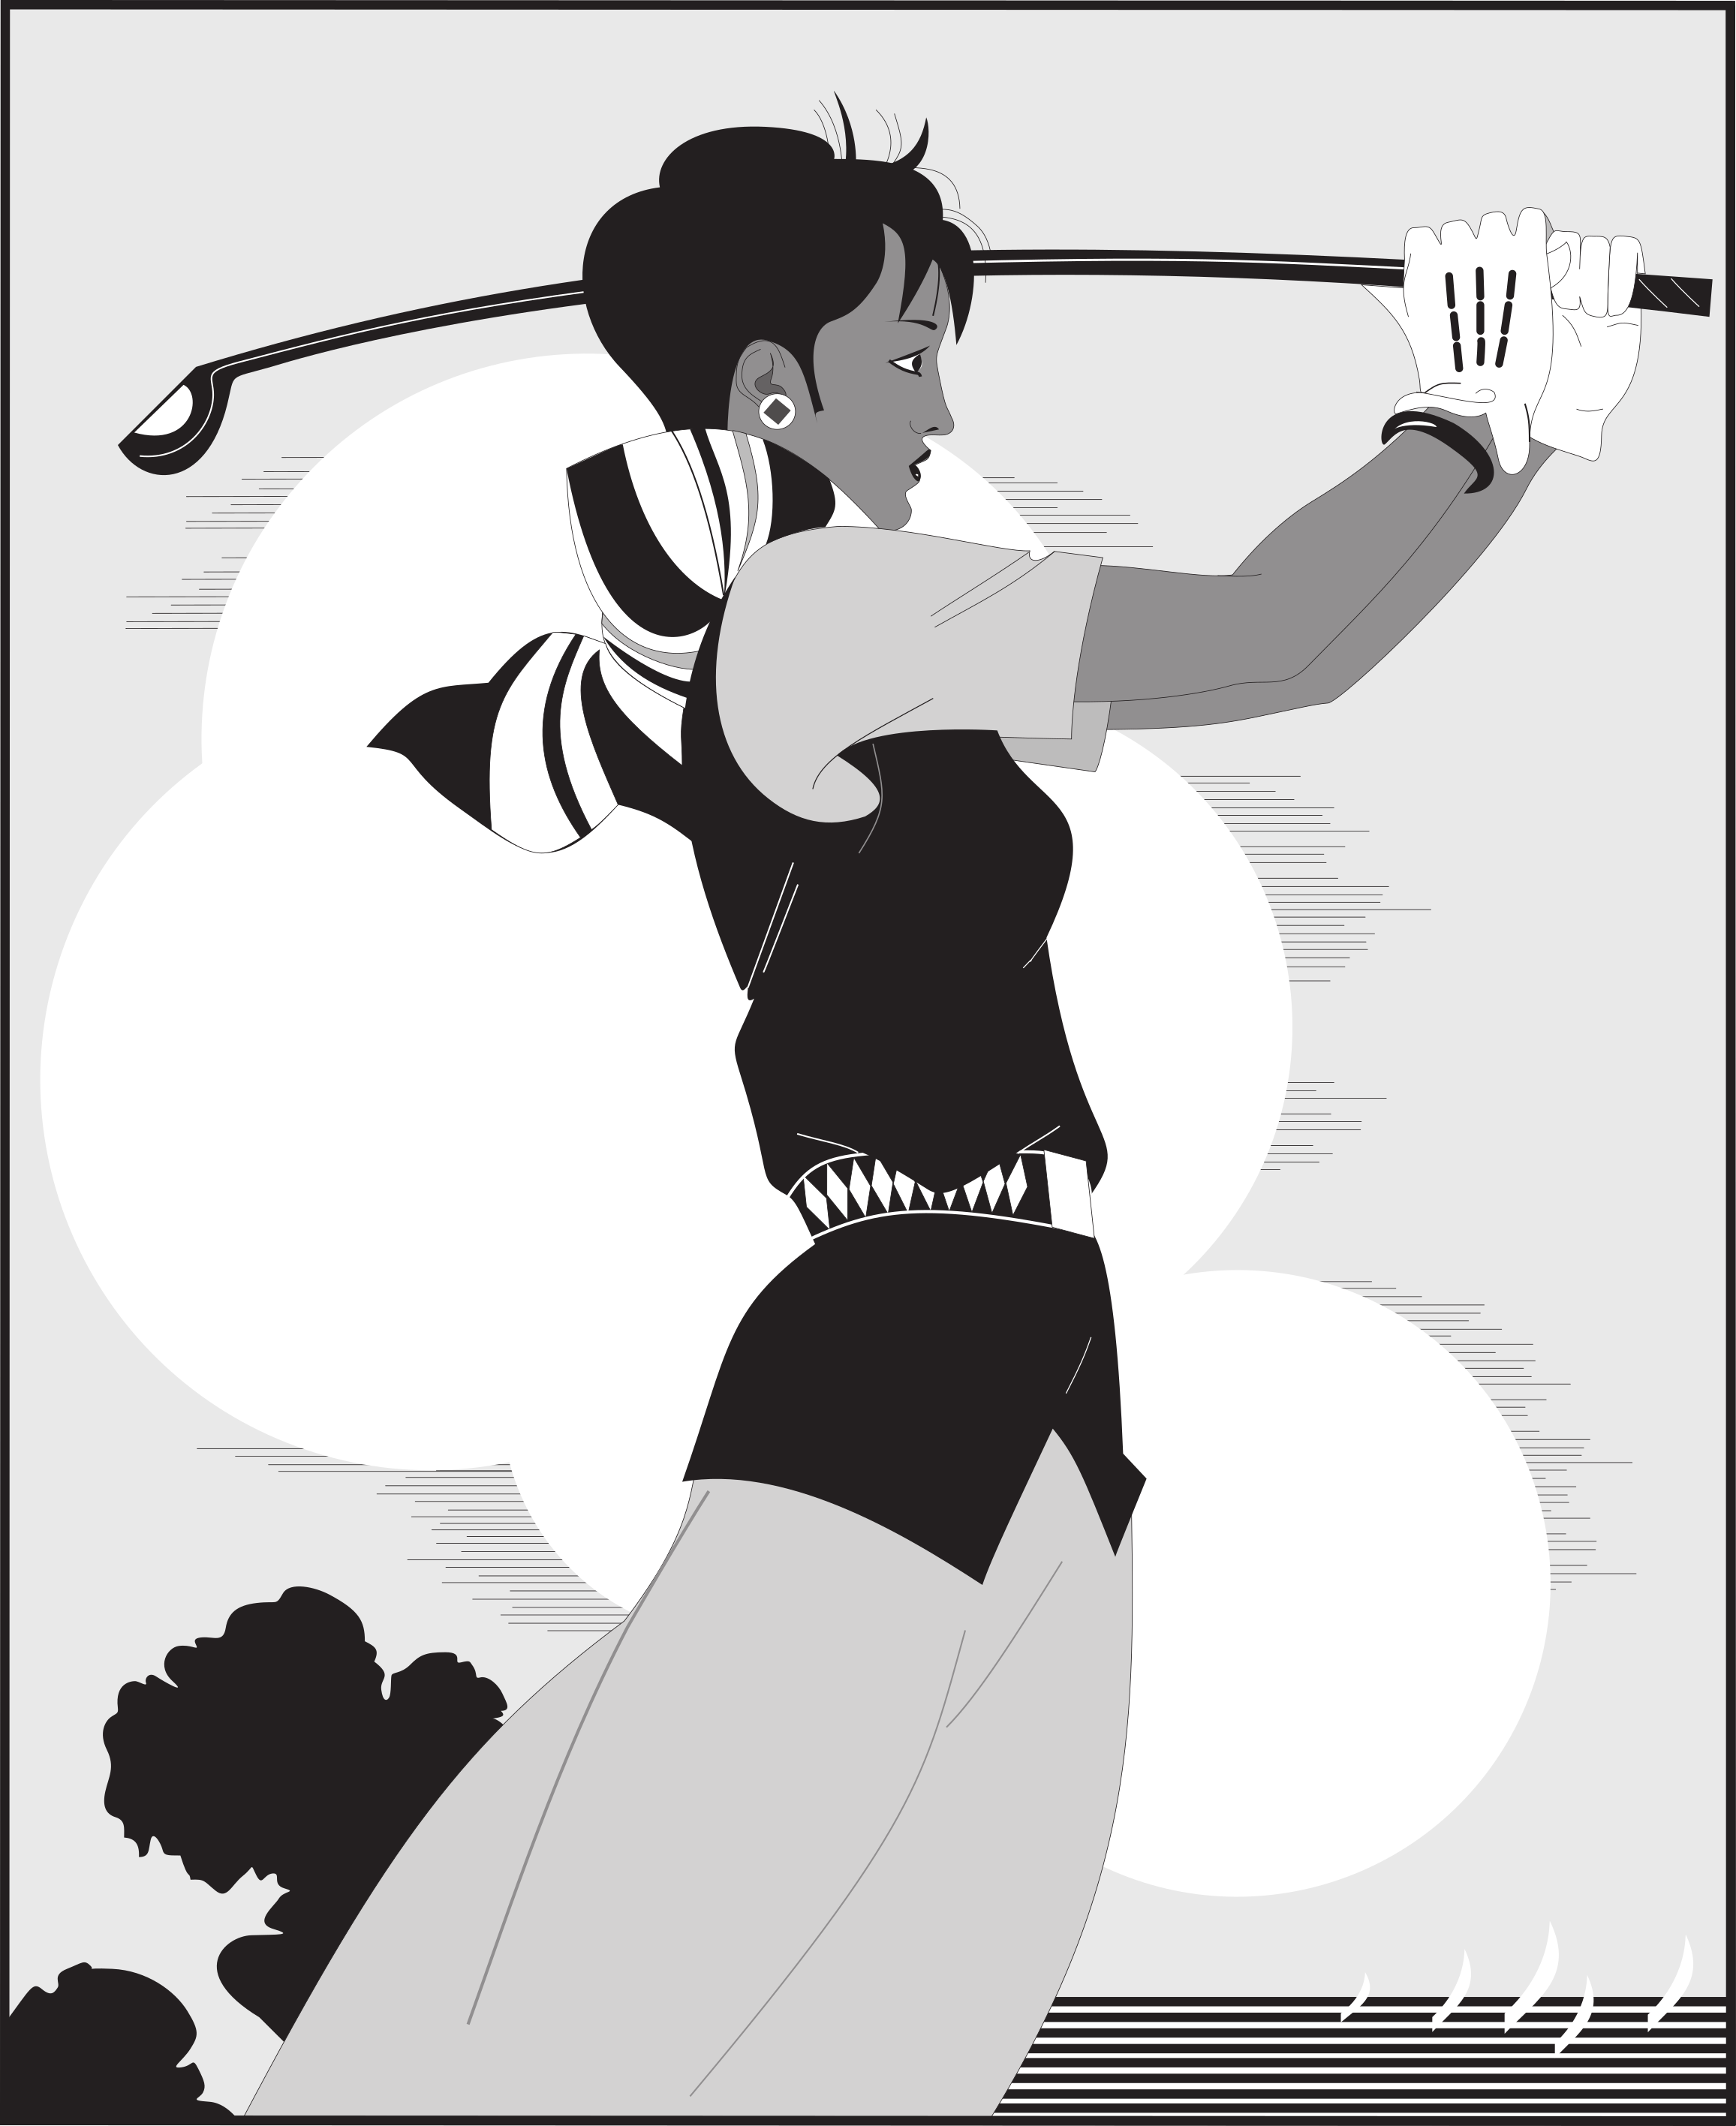
\includegraphics[width = 0.4\textwidth]{golfer}
\bicaption[golfer1]{}{打高尔夫球球的人(博士论文双语题注)}{Fig.$\!$}{The person playing golf (Doctoral thesis)}
\end{figure}

每个图均应有图题(由图序和图名组成),图题不宜有标点符号,图名在图序之后空1个半
角字符排写。图序按章编排,如第1章第一个插图的图号为“图1-1”。图题置于图下,硕士论
文只用中文,博士论文用中、英两种文字,居中书写,中文在上,要求中文用宋体5号字,
英文用Times New Roman 5号字。有图注或其它说明时应置于图题之上。引用图应注明出处
,在图题右上角加引用文献号。图中若有分图时,分图题置于分图之下或图题之下,可以只
用中文书写,分图号用a)、b)等表示。图中各部分说明应采用中文(引用的外文图除外)或
数字符号,各项文字说明置于图题之上(有分图时,置于分图题之上)。图中文字用宋体、
Times New Roman字体,字号尽量采用5号字(当字数较多时可用小5号字,以清晰表达为原
则,但在一个插图内字号要统一)。同一图内使用文字应统一。图表中物理量、符号用斜体
。
\subsection{本硕论文题注}[Other picture example]
\begin{figure}[h]
\centering
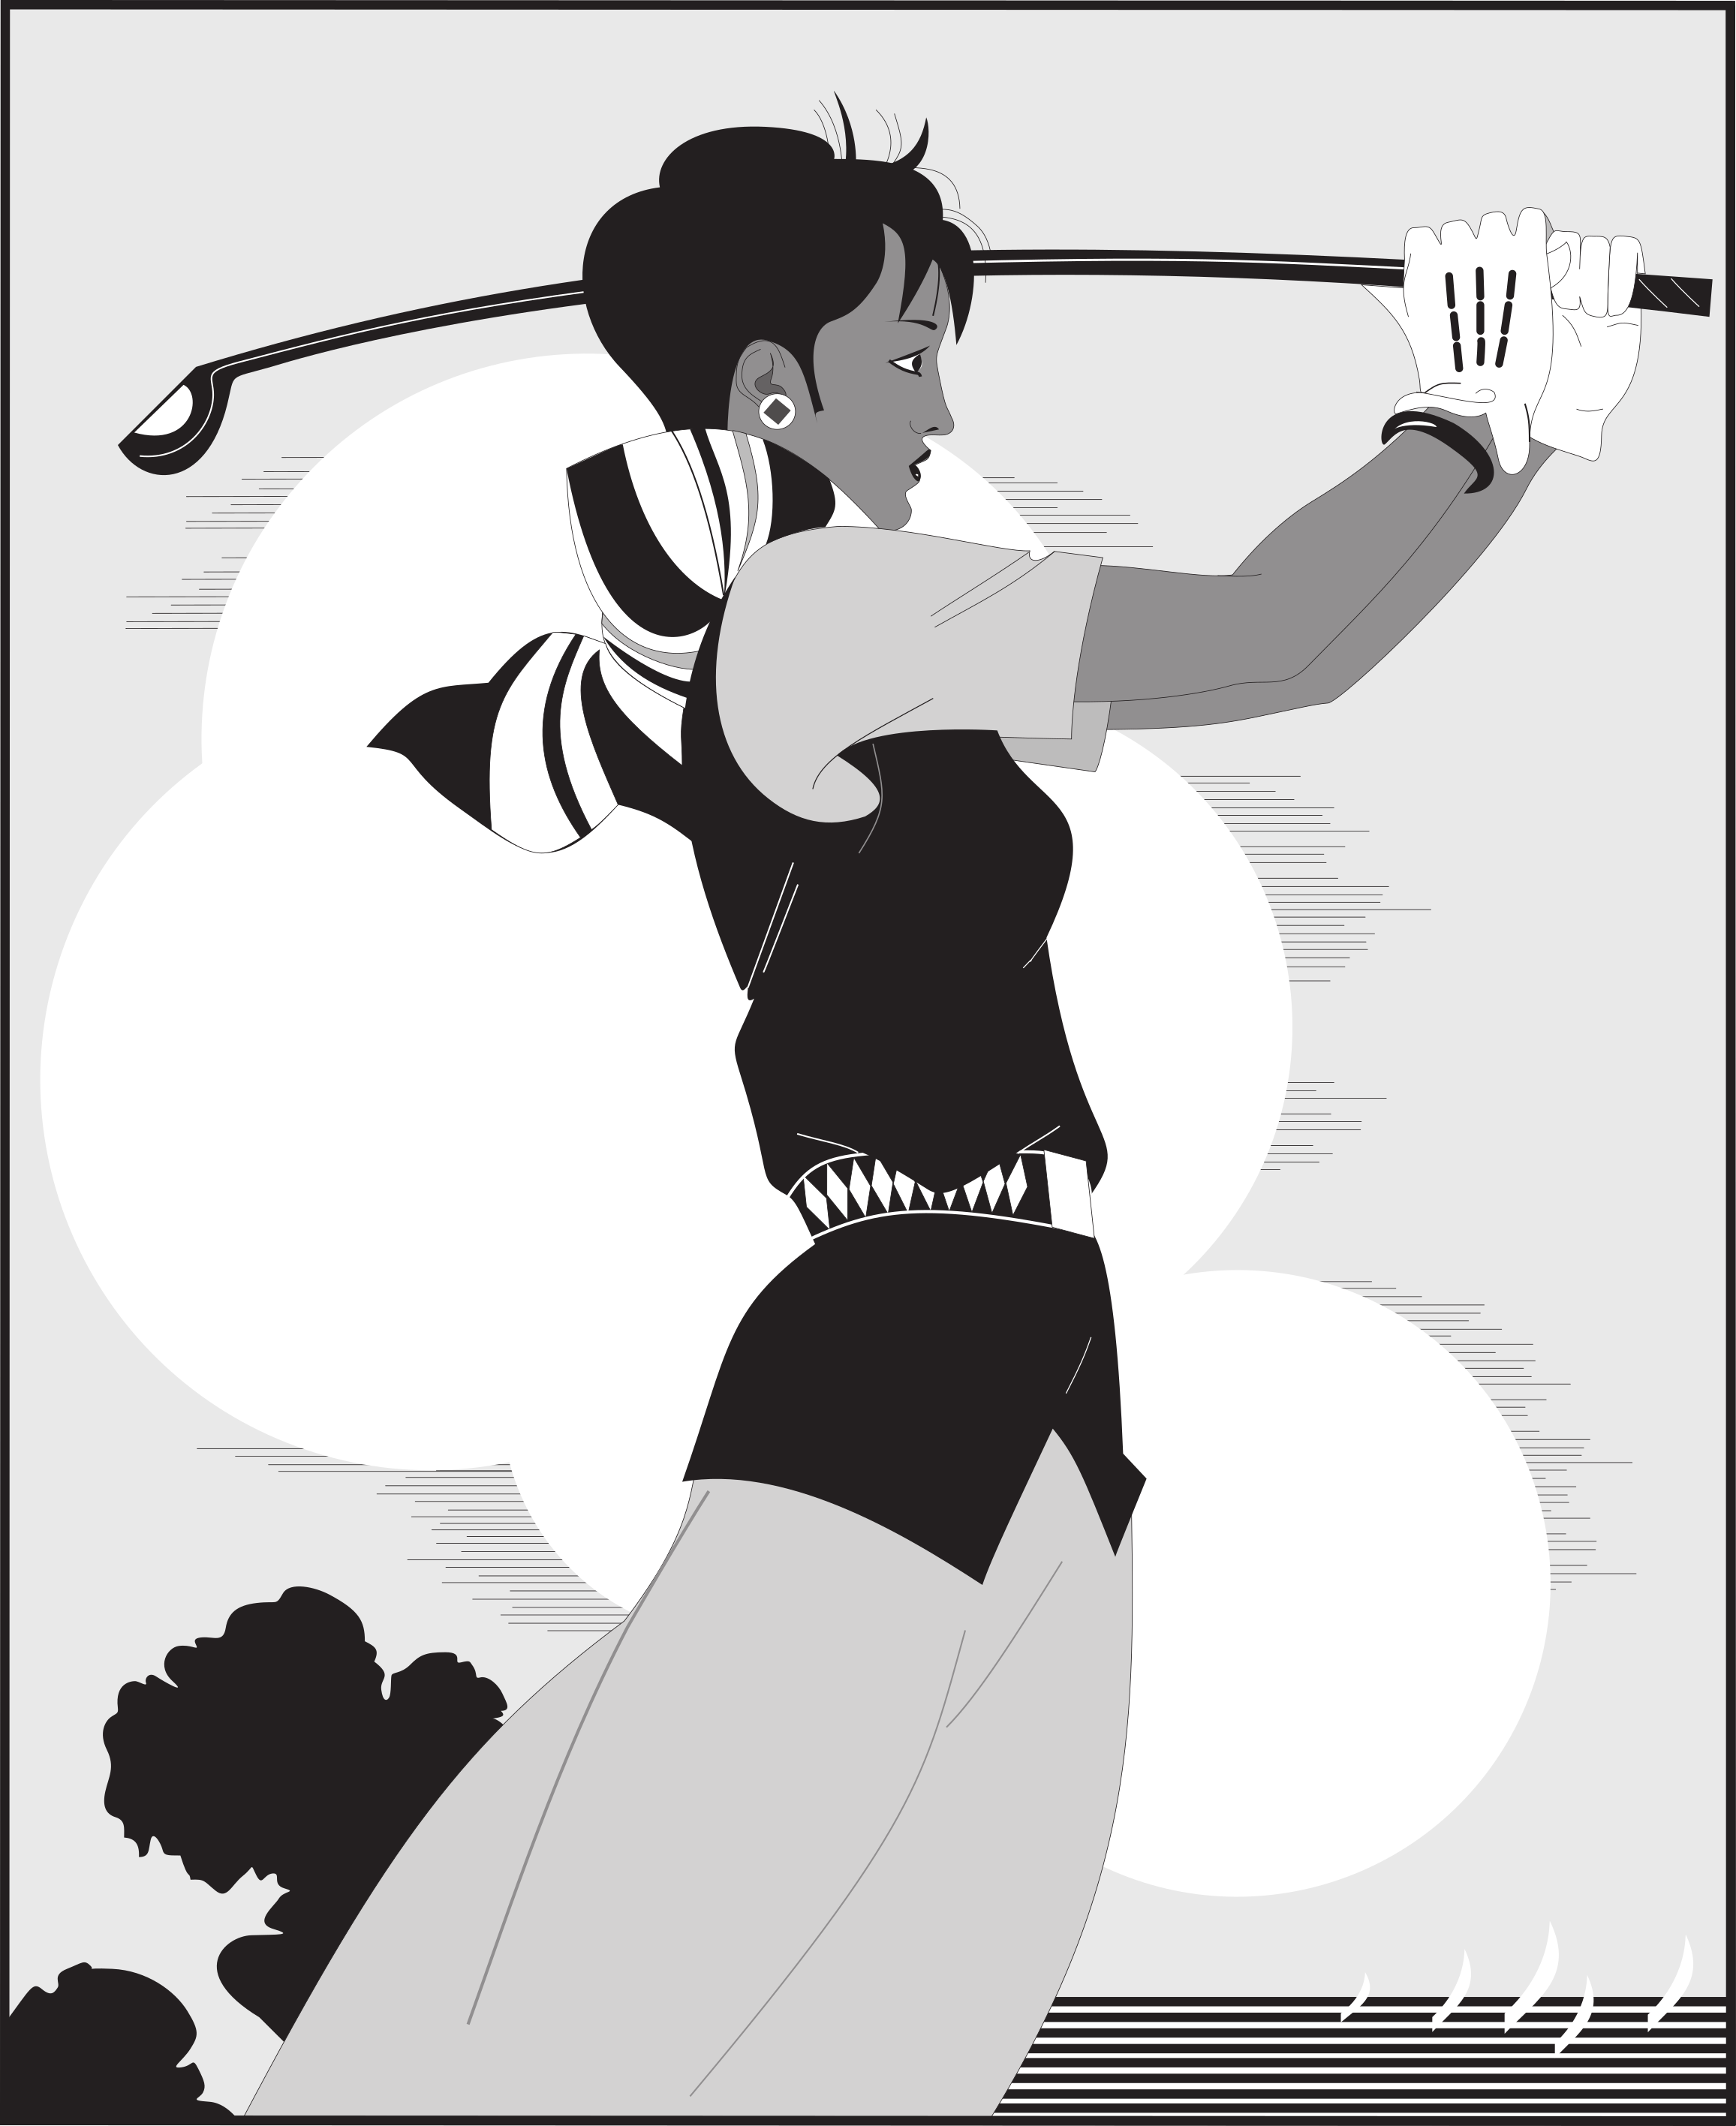
\includegraphics[width = 0.4\textwidth]{golfer}
\caption{打高尔夫球的人,硕士论文要求只用汉语}
\end{figure}

\subsection{并排图和子图}[Abreast-picture and Sub-picture example]
\subsubsection{并排图}[Abreast-picture example]

使用并排图时,需要注意对齐方式。默认情况是中部对齐。这里给出中部对齐、顶部对齐
、图片底部对齐三种常见方式。其中,底部对齐方式有一个很巧妙的方式,将长度比较小
的图放在左面即可。

\begin{figure}[htbp]
\centering
\begin{minipage}{0.4\textwidth}
\centering
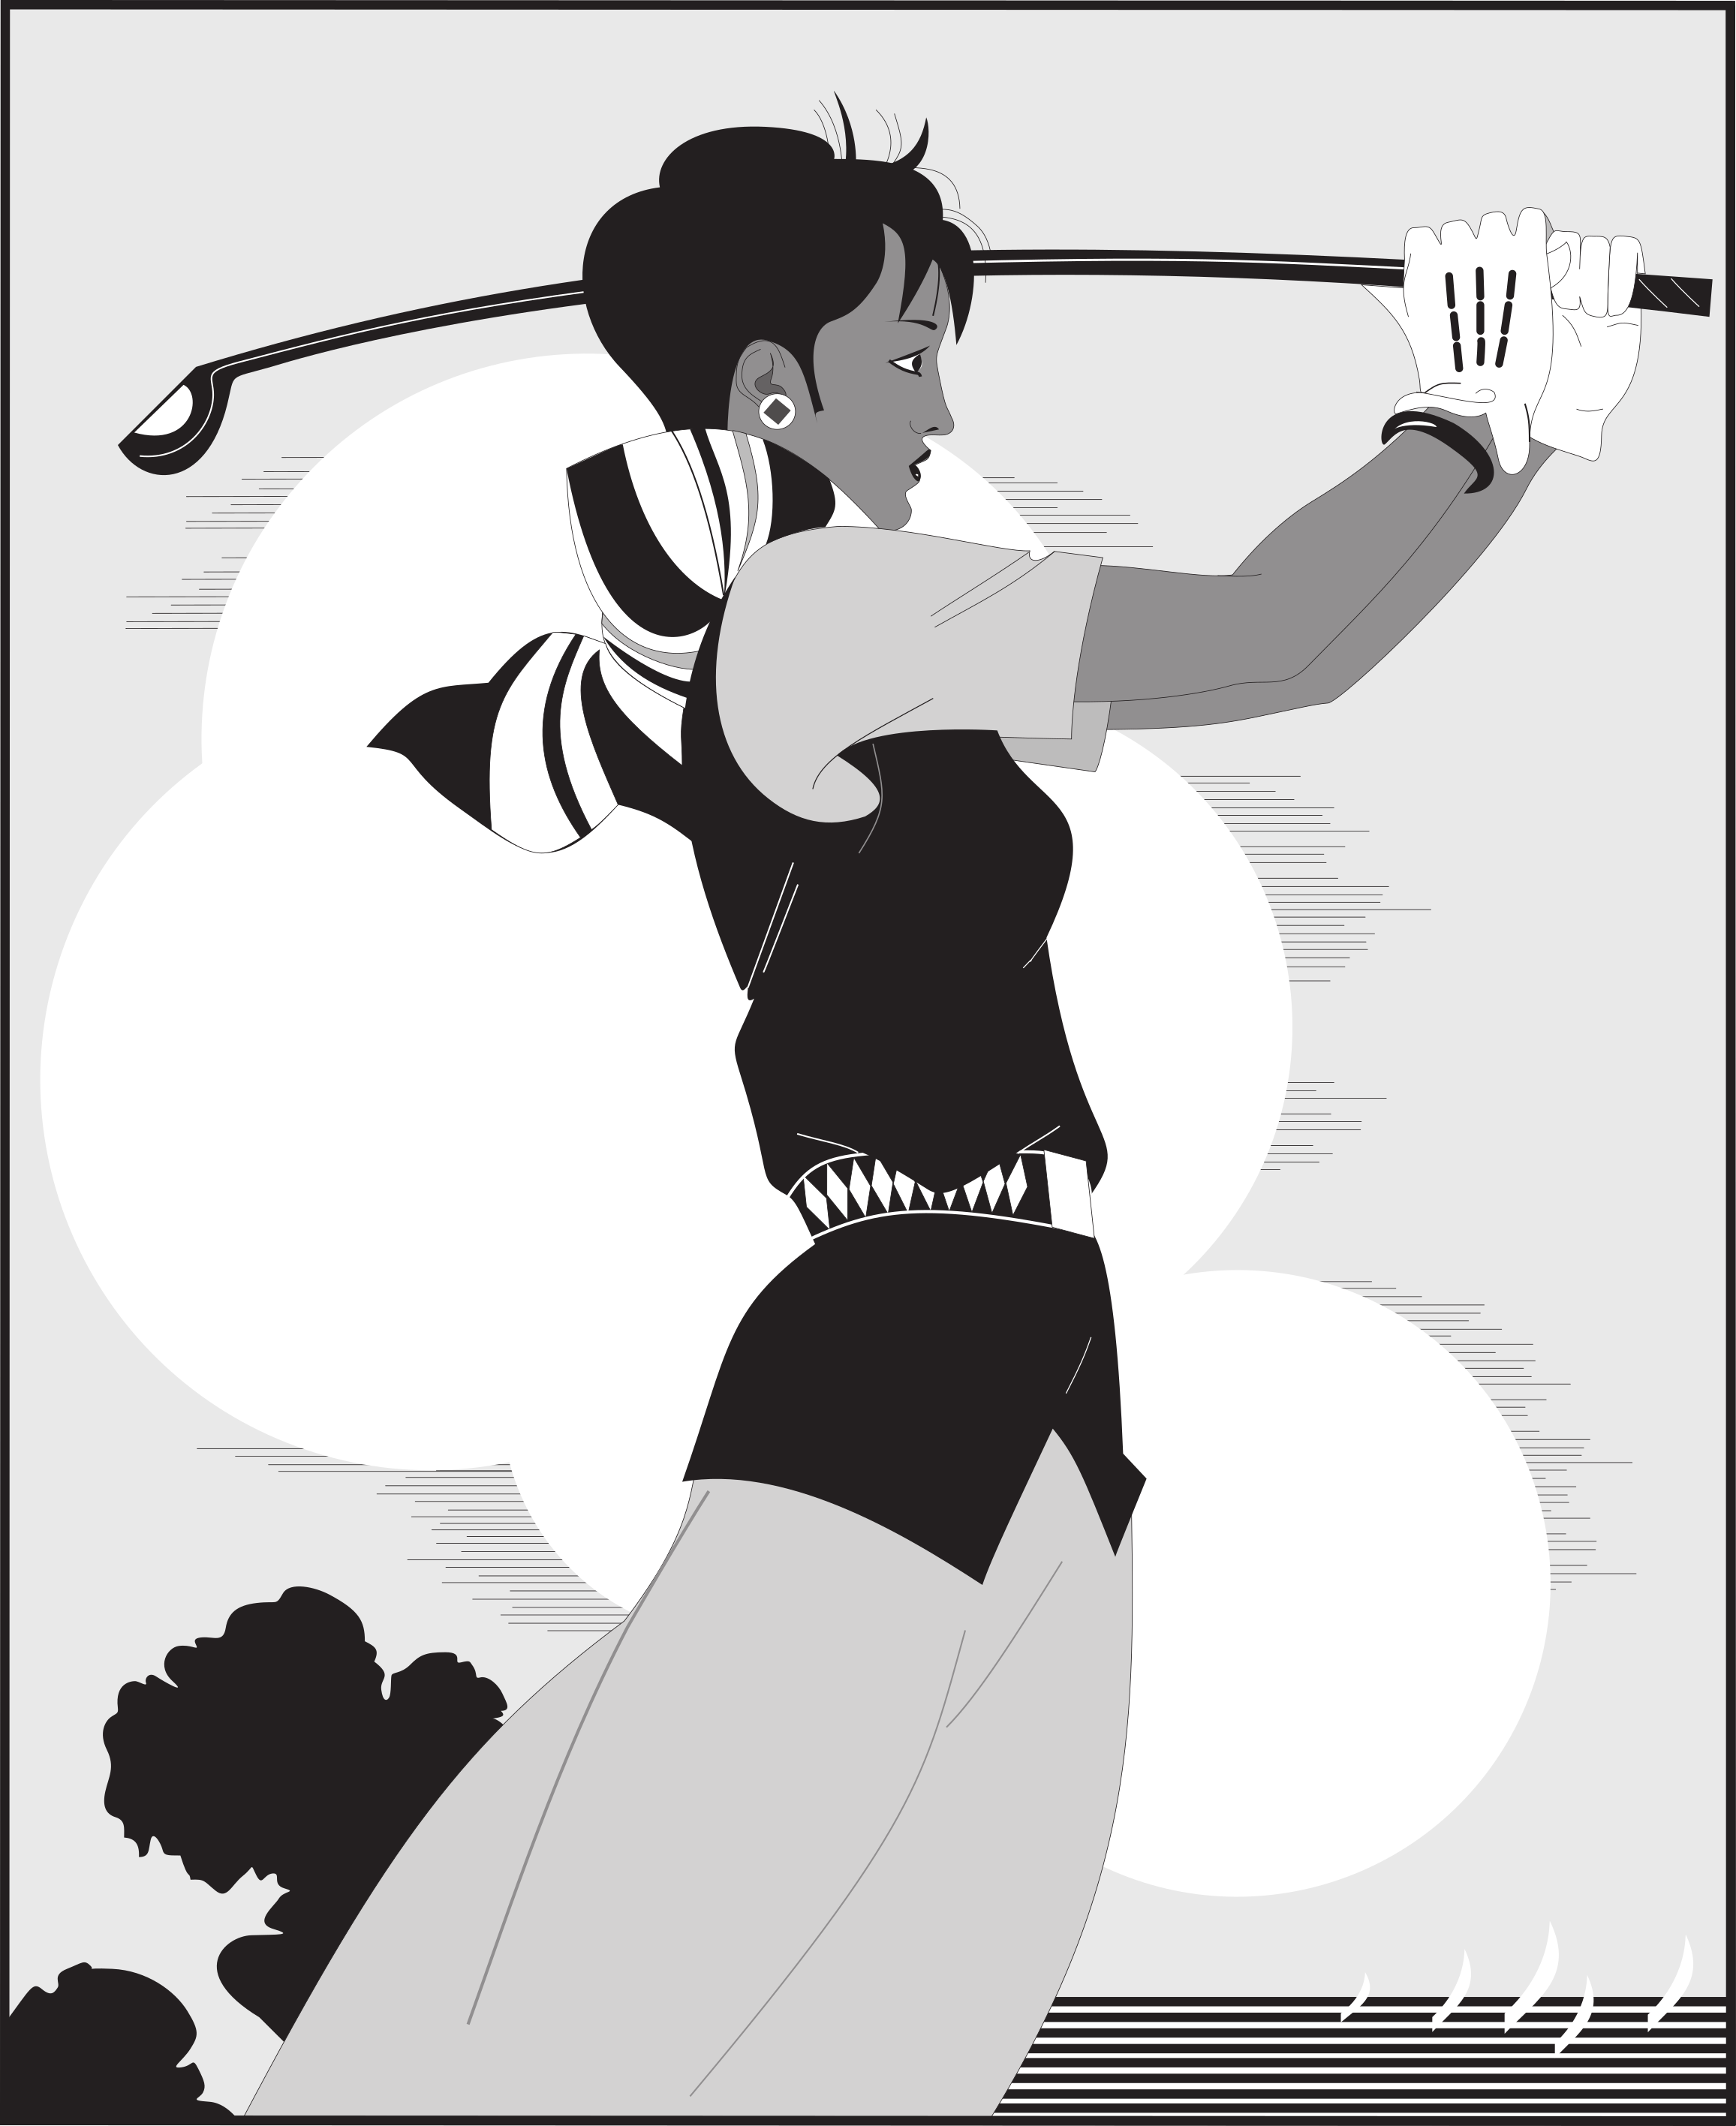
\includegraphics[width=\textwidth]{golfer}
\bicaption[golfer2]{}{打高尔夫球的人}{Fig.$\!$}{The person playing golf}
\end{minipage}
\centering
\begin{minipage}{0.4\textwidth}
\centering
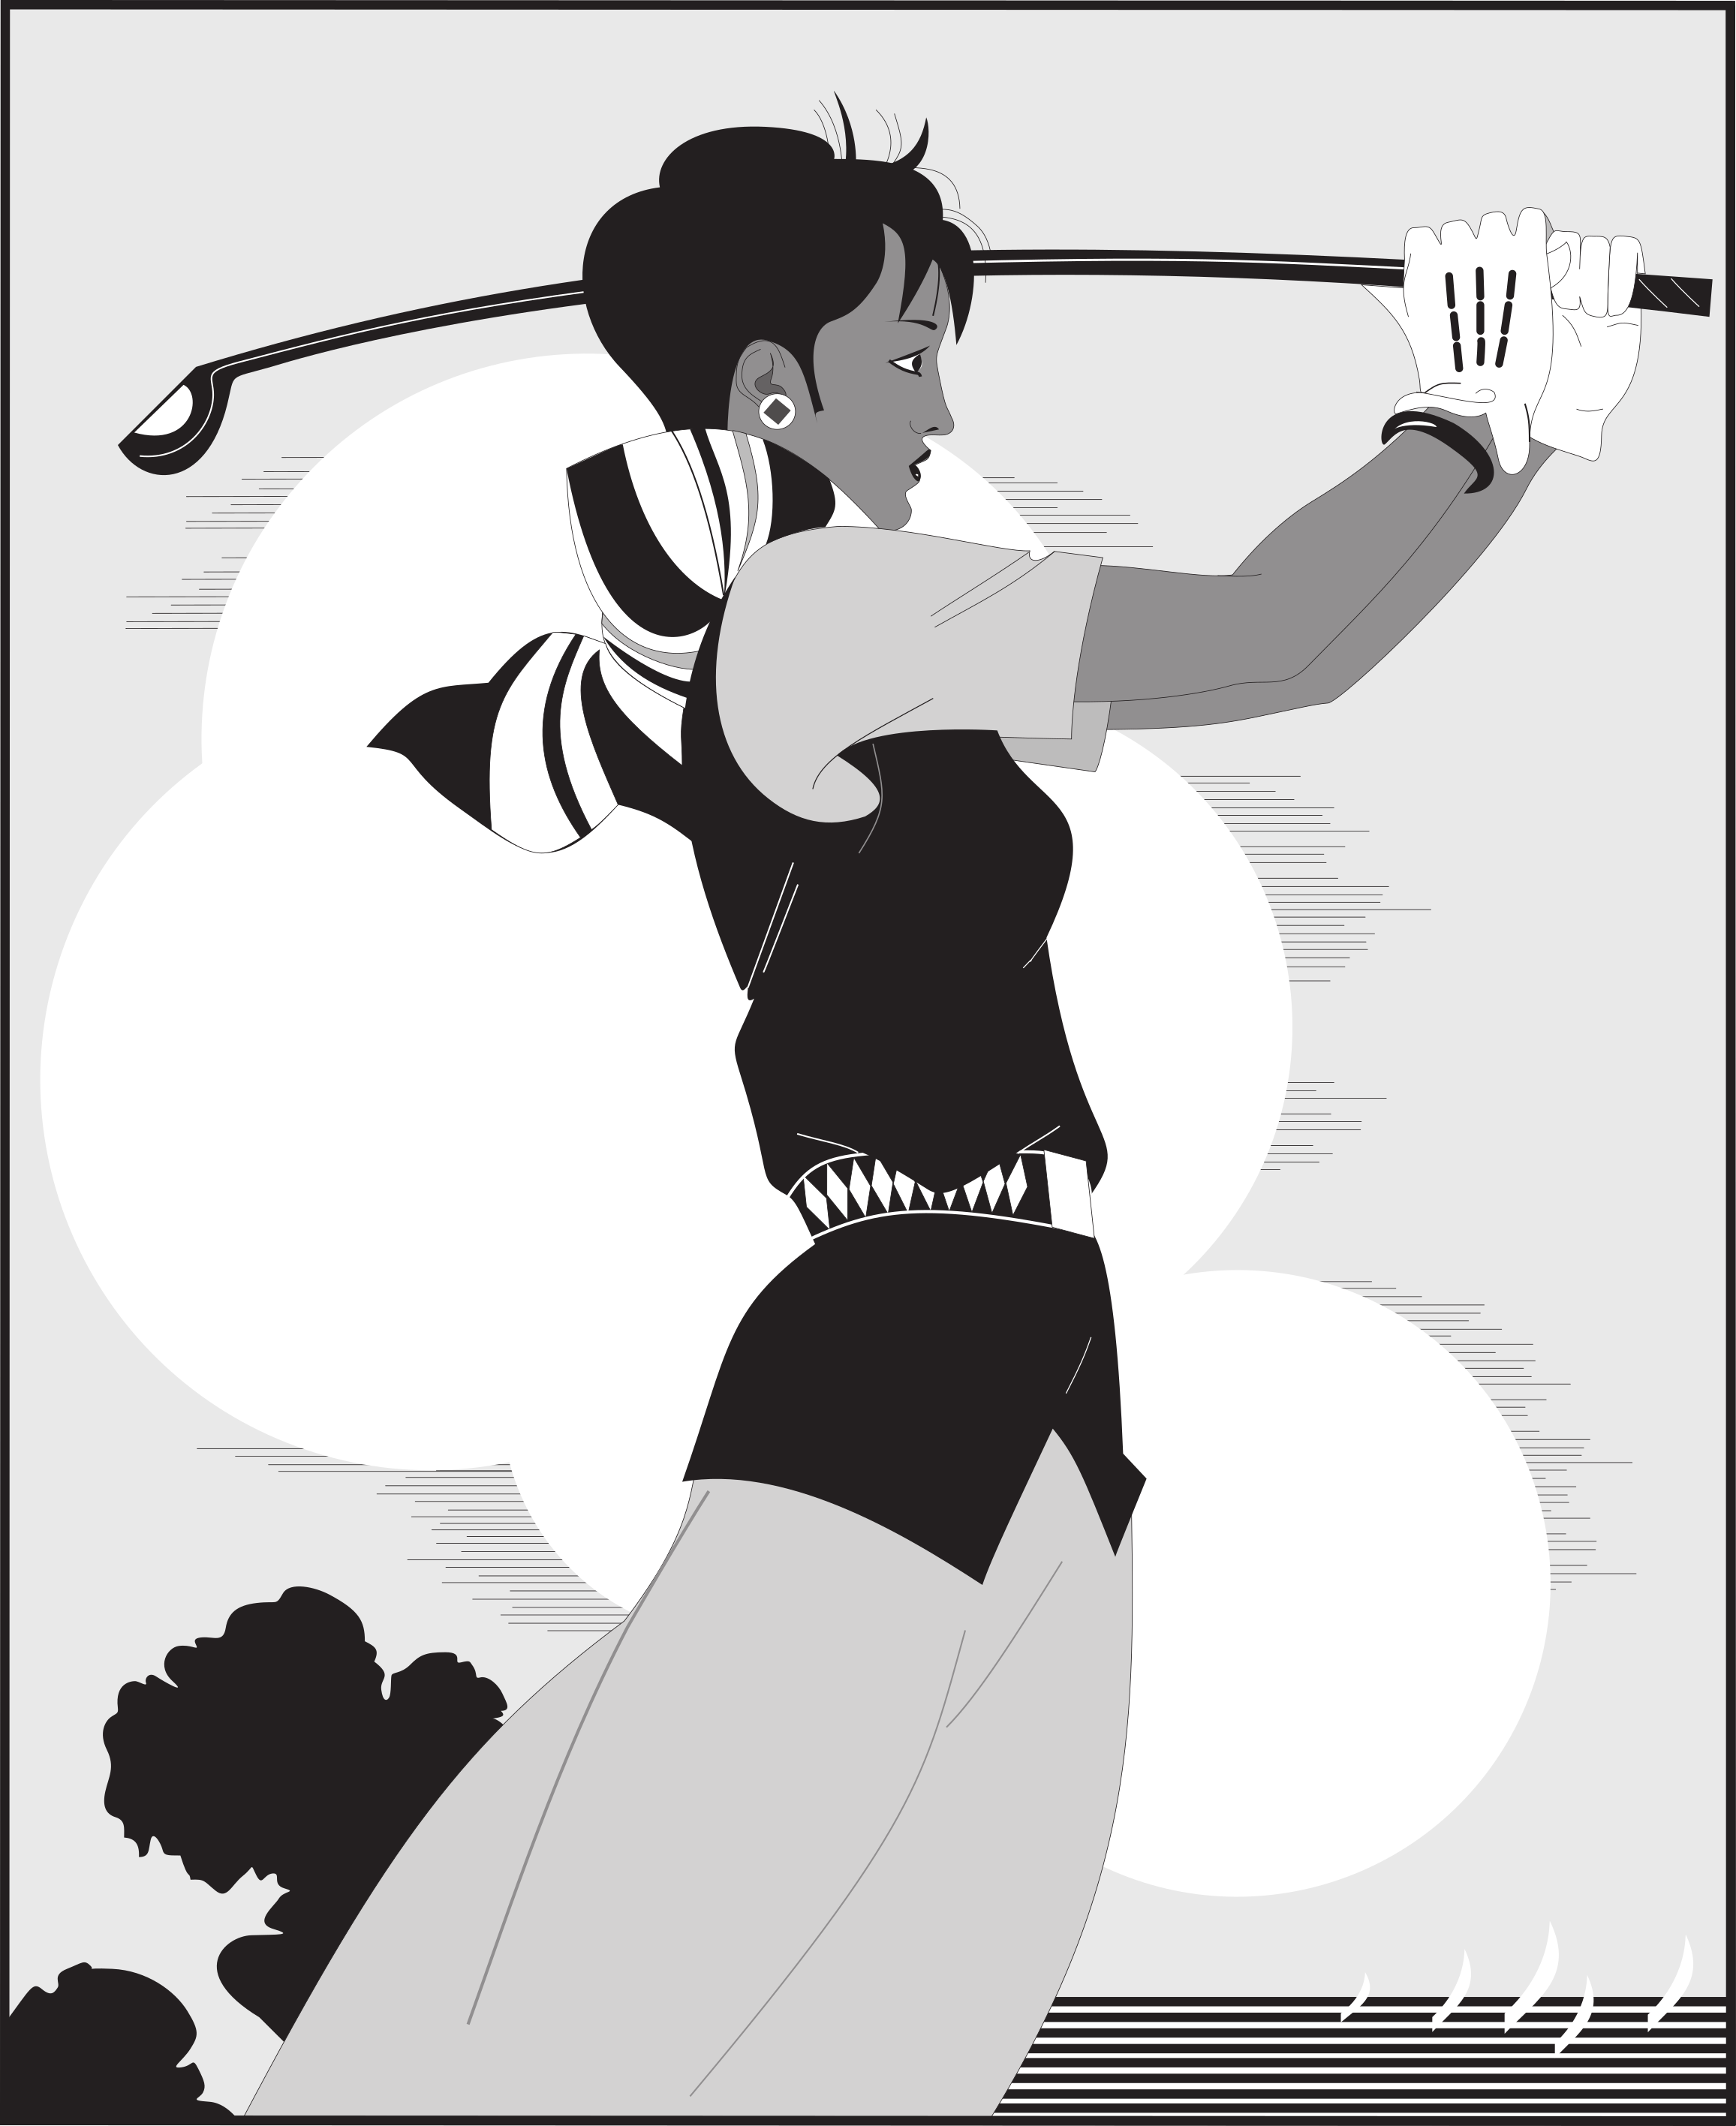
\includegraphics[width=\textwidth]{golfer}
\bicaption[golfer3]{}{打高尔夫球的人。注意,这里默认居中}{Fig.$\!$}{The person playing golf. Please note that, it is vertically center aligned by default.}
\end{minipage}
\end{figure}

\begin{figure}[htbp]
\centering
\begin{minipage}[t]{0.4\textwidth}
\centering
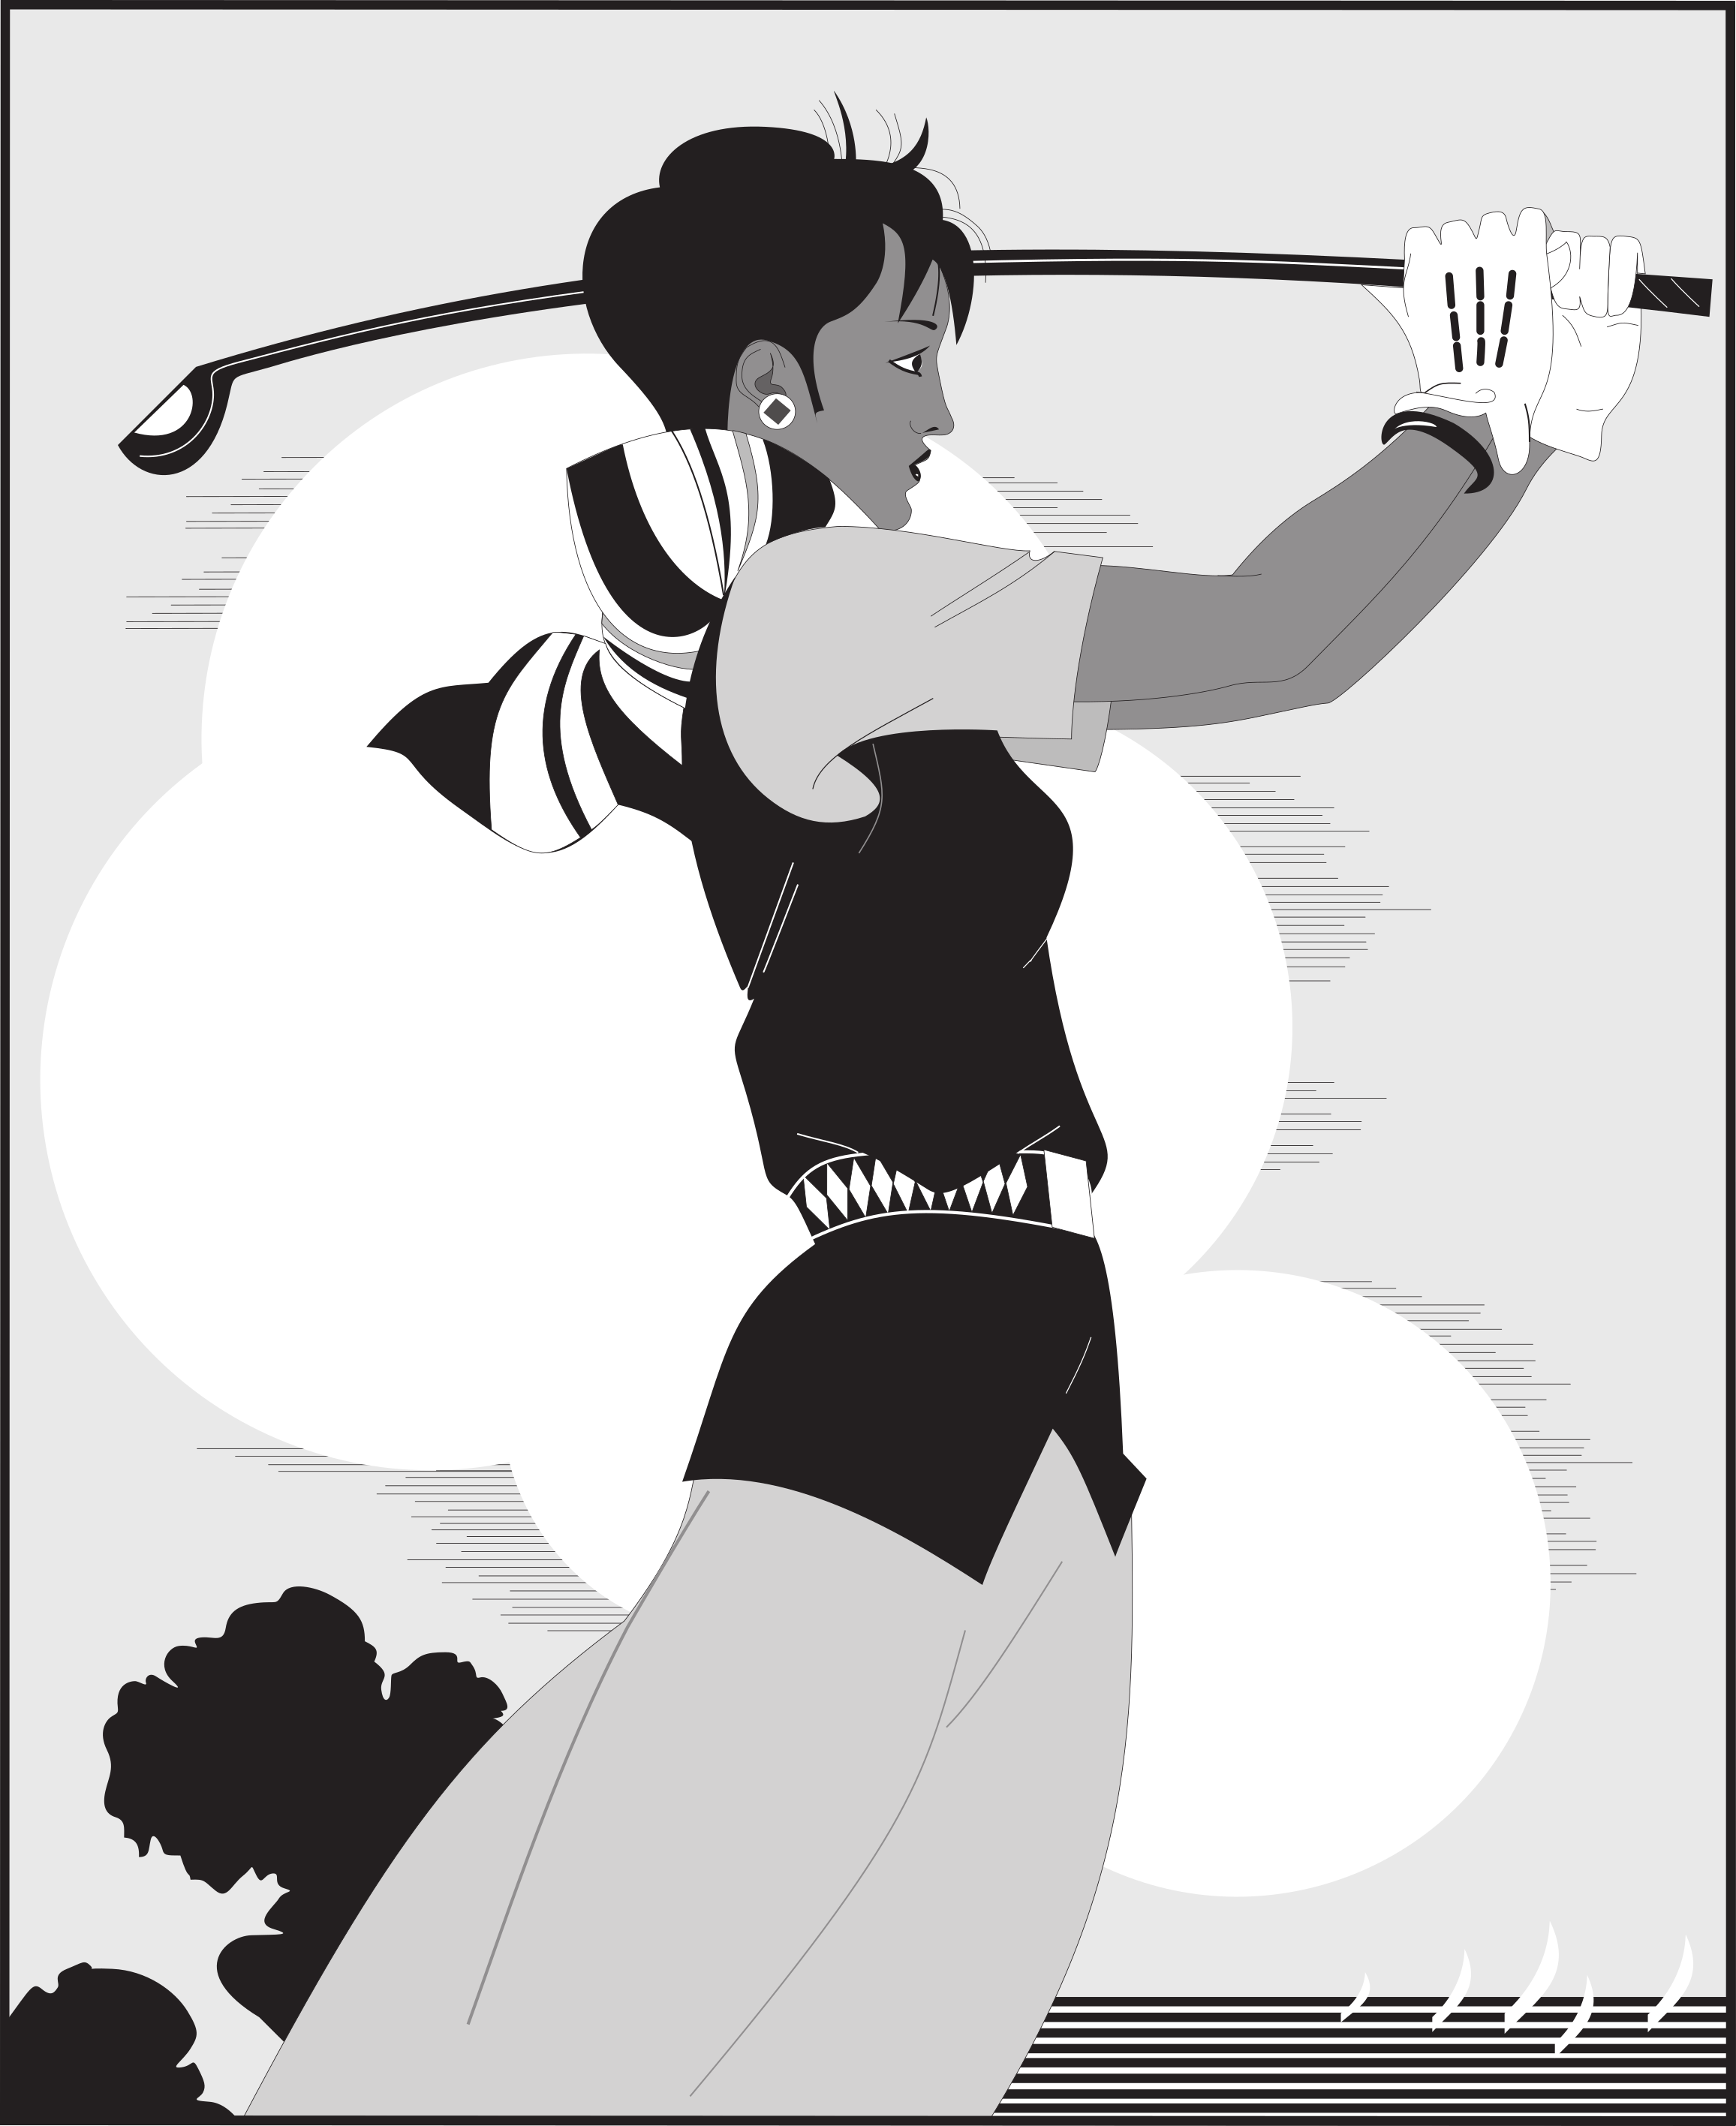
\includegraphics[width=\textwidth]{golfer}
\bicaption[golfer5]{}{打高尔夫球的人}{Fig.$\!$}{The person playing golf}
\end{minipage}
\centering
\begin{minipage}[t]{0.4\textwidth}
\centering
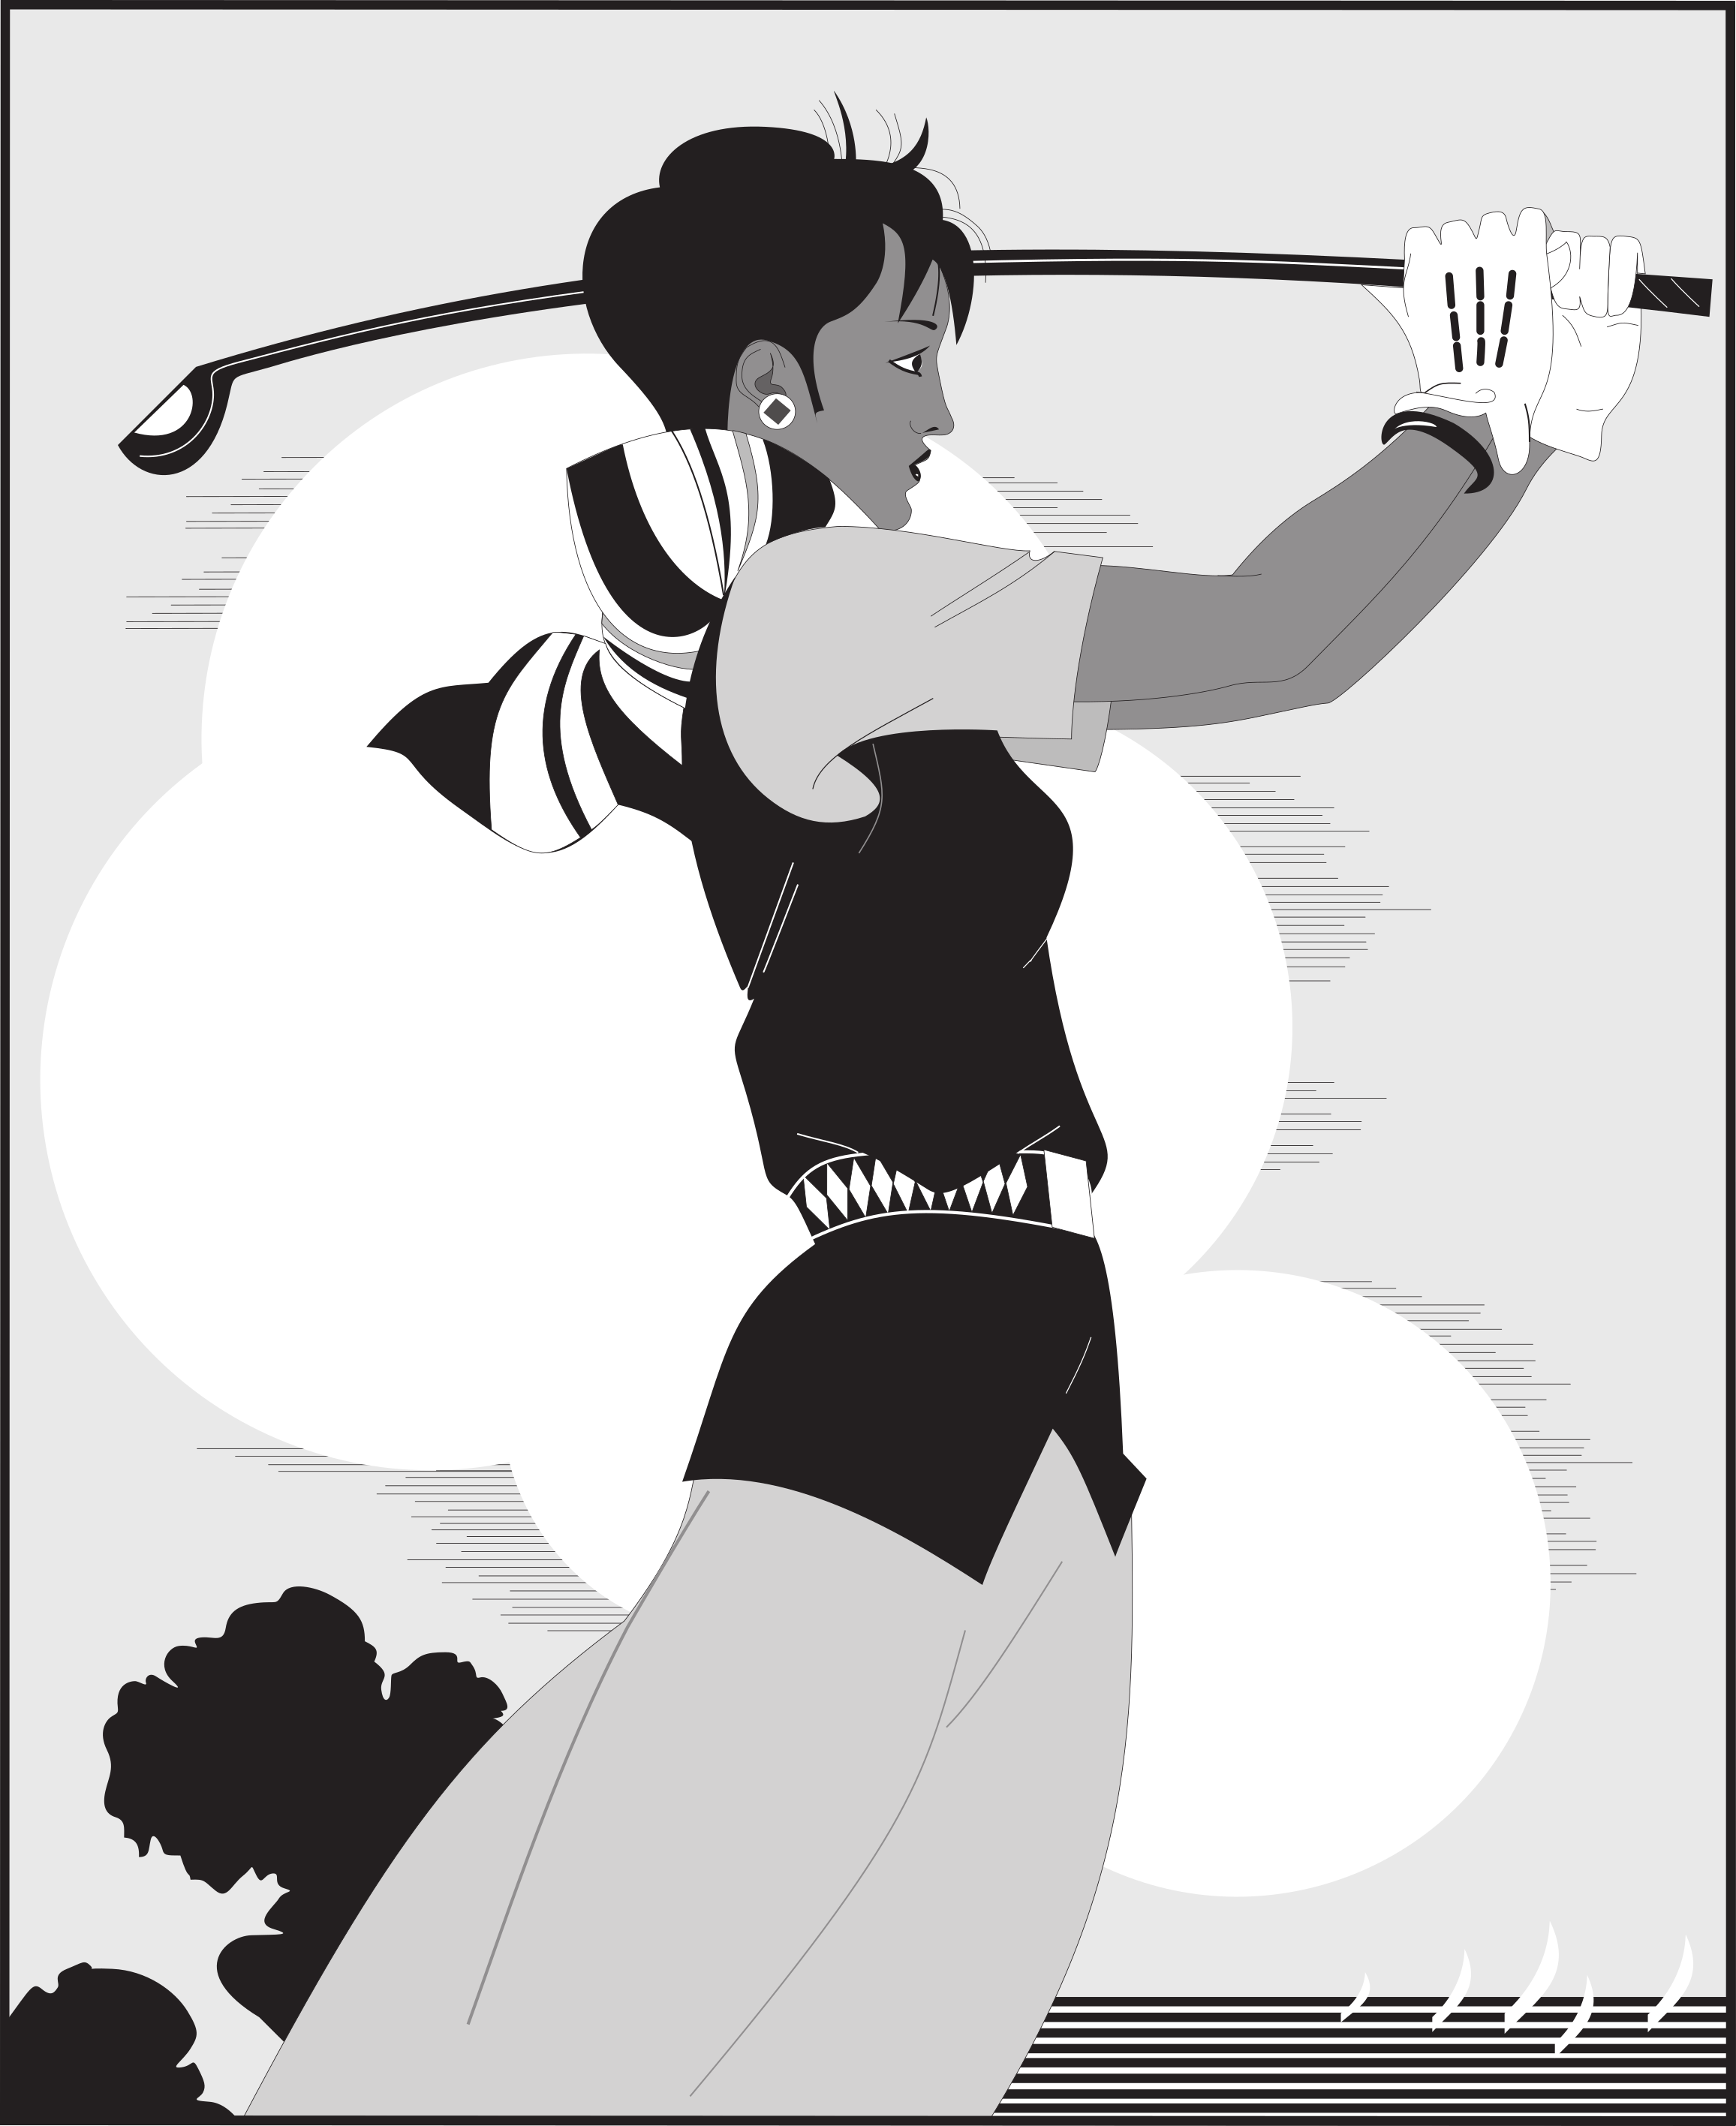
\includegraphics[width=\textwidth]{golfer}
\bicaption[golfer8]{}{打高尔夫球的人。注意,此图是顶部对齐}{Fig.$\!$}{The person playing golf. Please note that, it is vertically top aligned.}
\end{minipage}
\end{figure}

\begin{figure}[htbp]
\centering
\begin{minipage}[t]{0.4\textwidth}
\centering
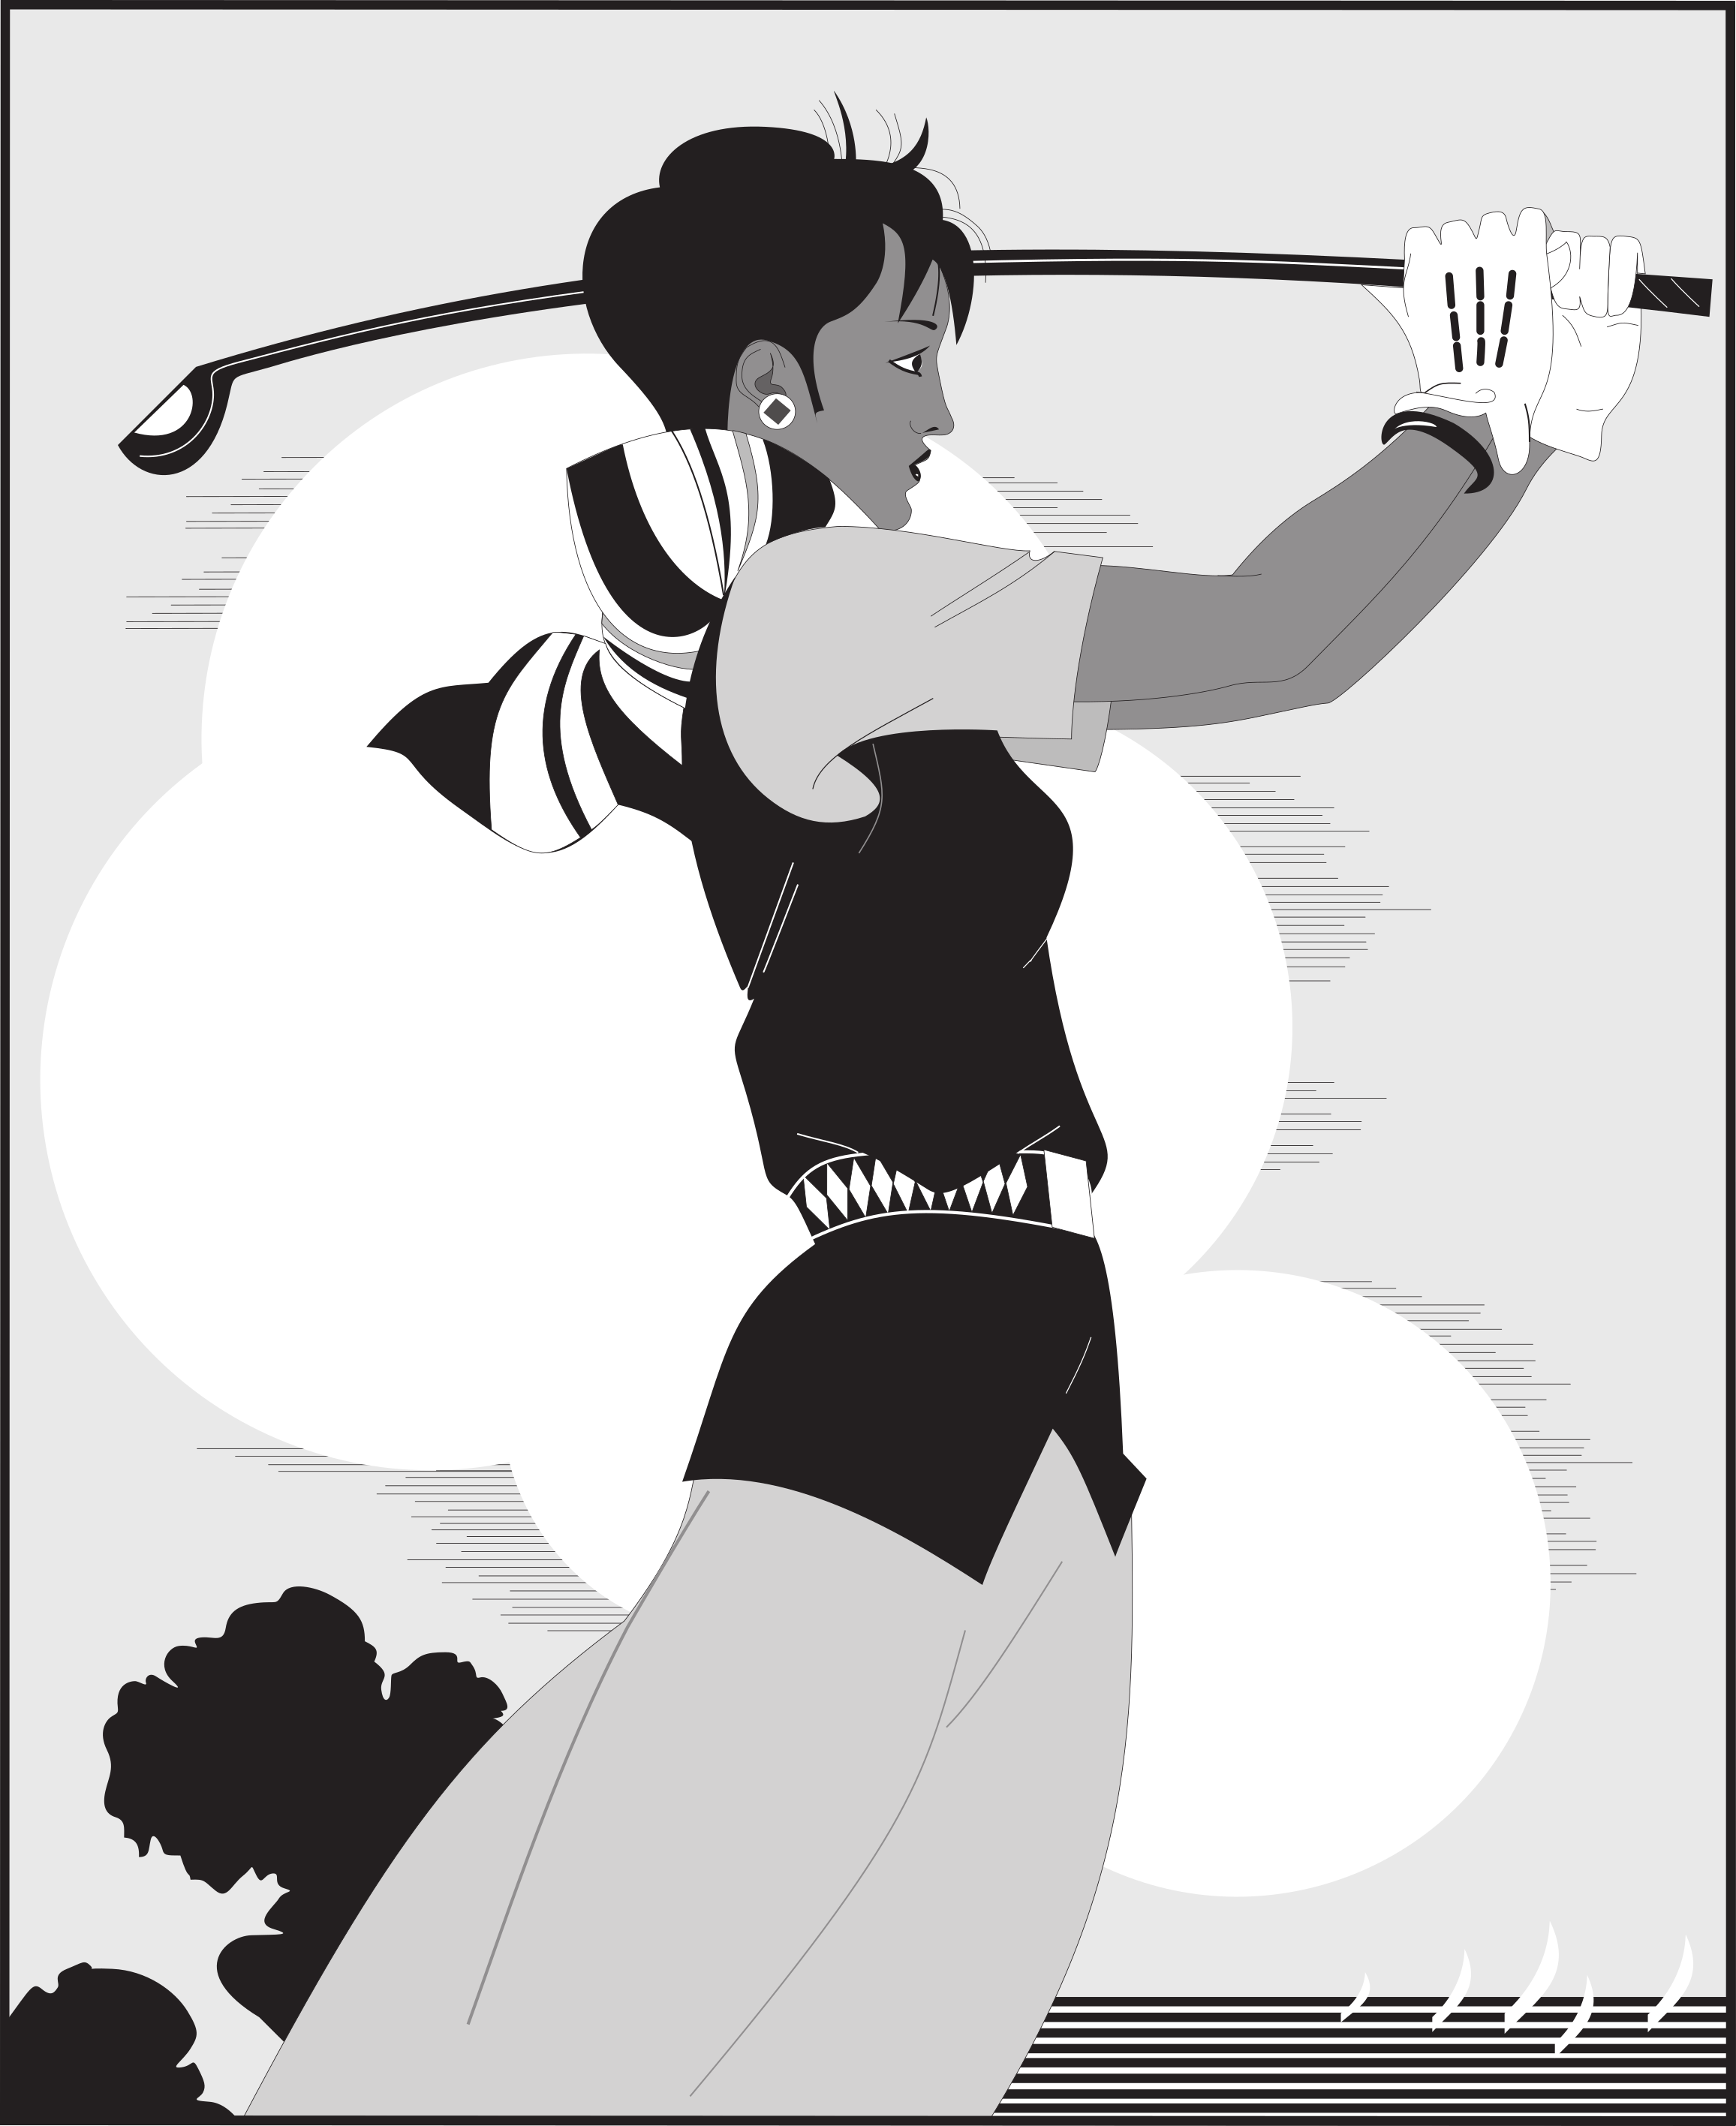
\includegraphics[width=\textwidth,height=\textwidth]{golfer}
\bicaption[golfer9]{}{打高尔夫球的人。注意,此图对齐方式是图片底部对齐}{Fig.$\!$}{The person playing golf. Please note that, it is vertically bottom aligned for figure.}
\end{minipage}
\centering
\begin{minipage}[t]{0.4\textwidth}
\centering
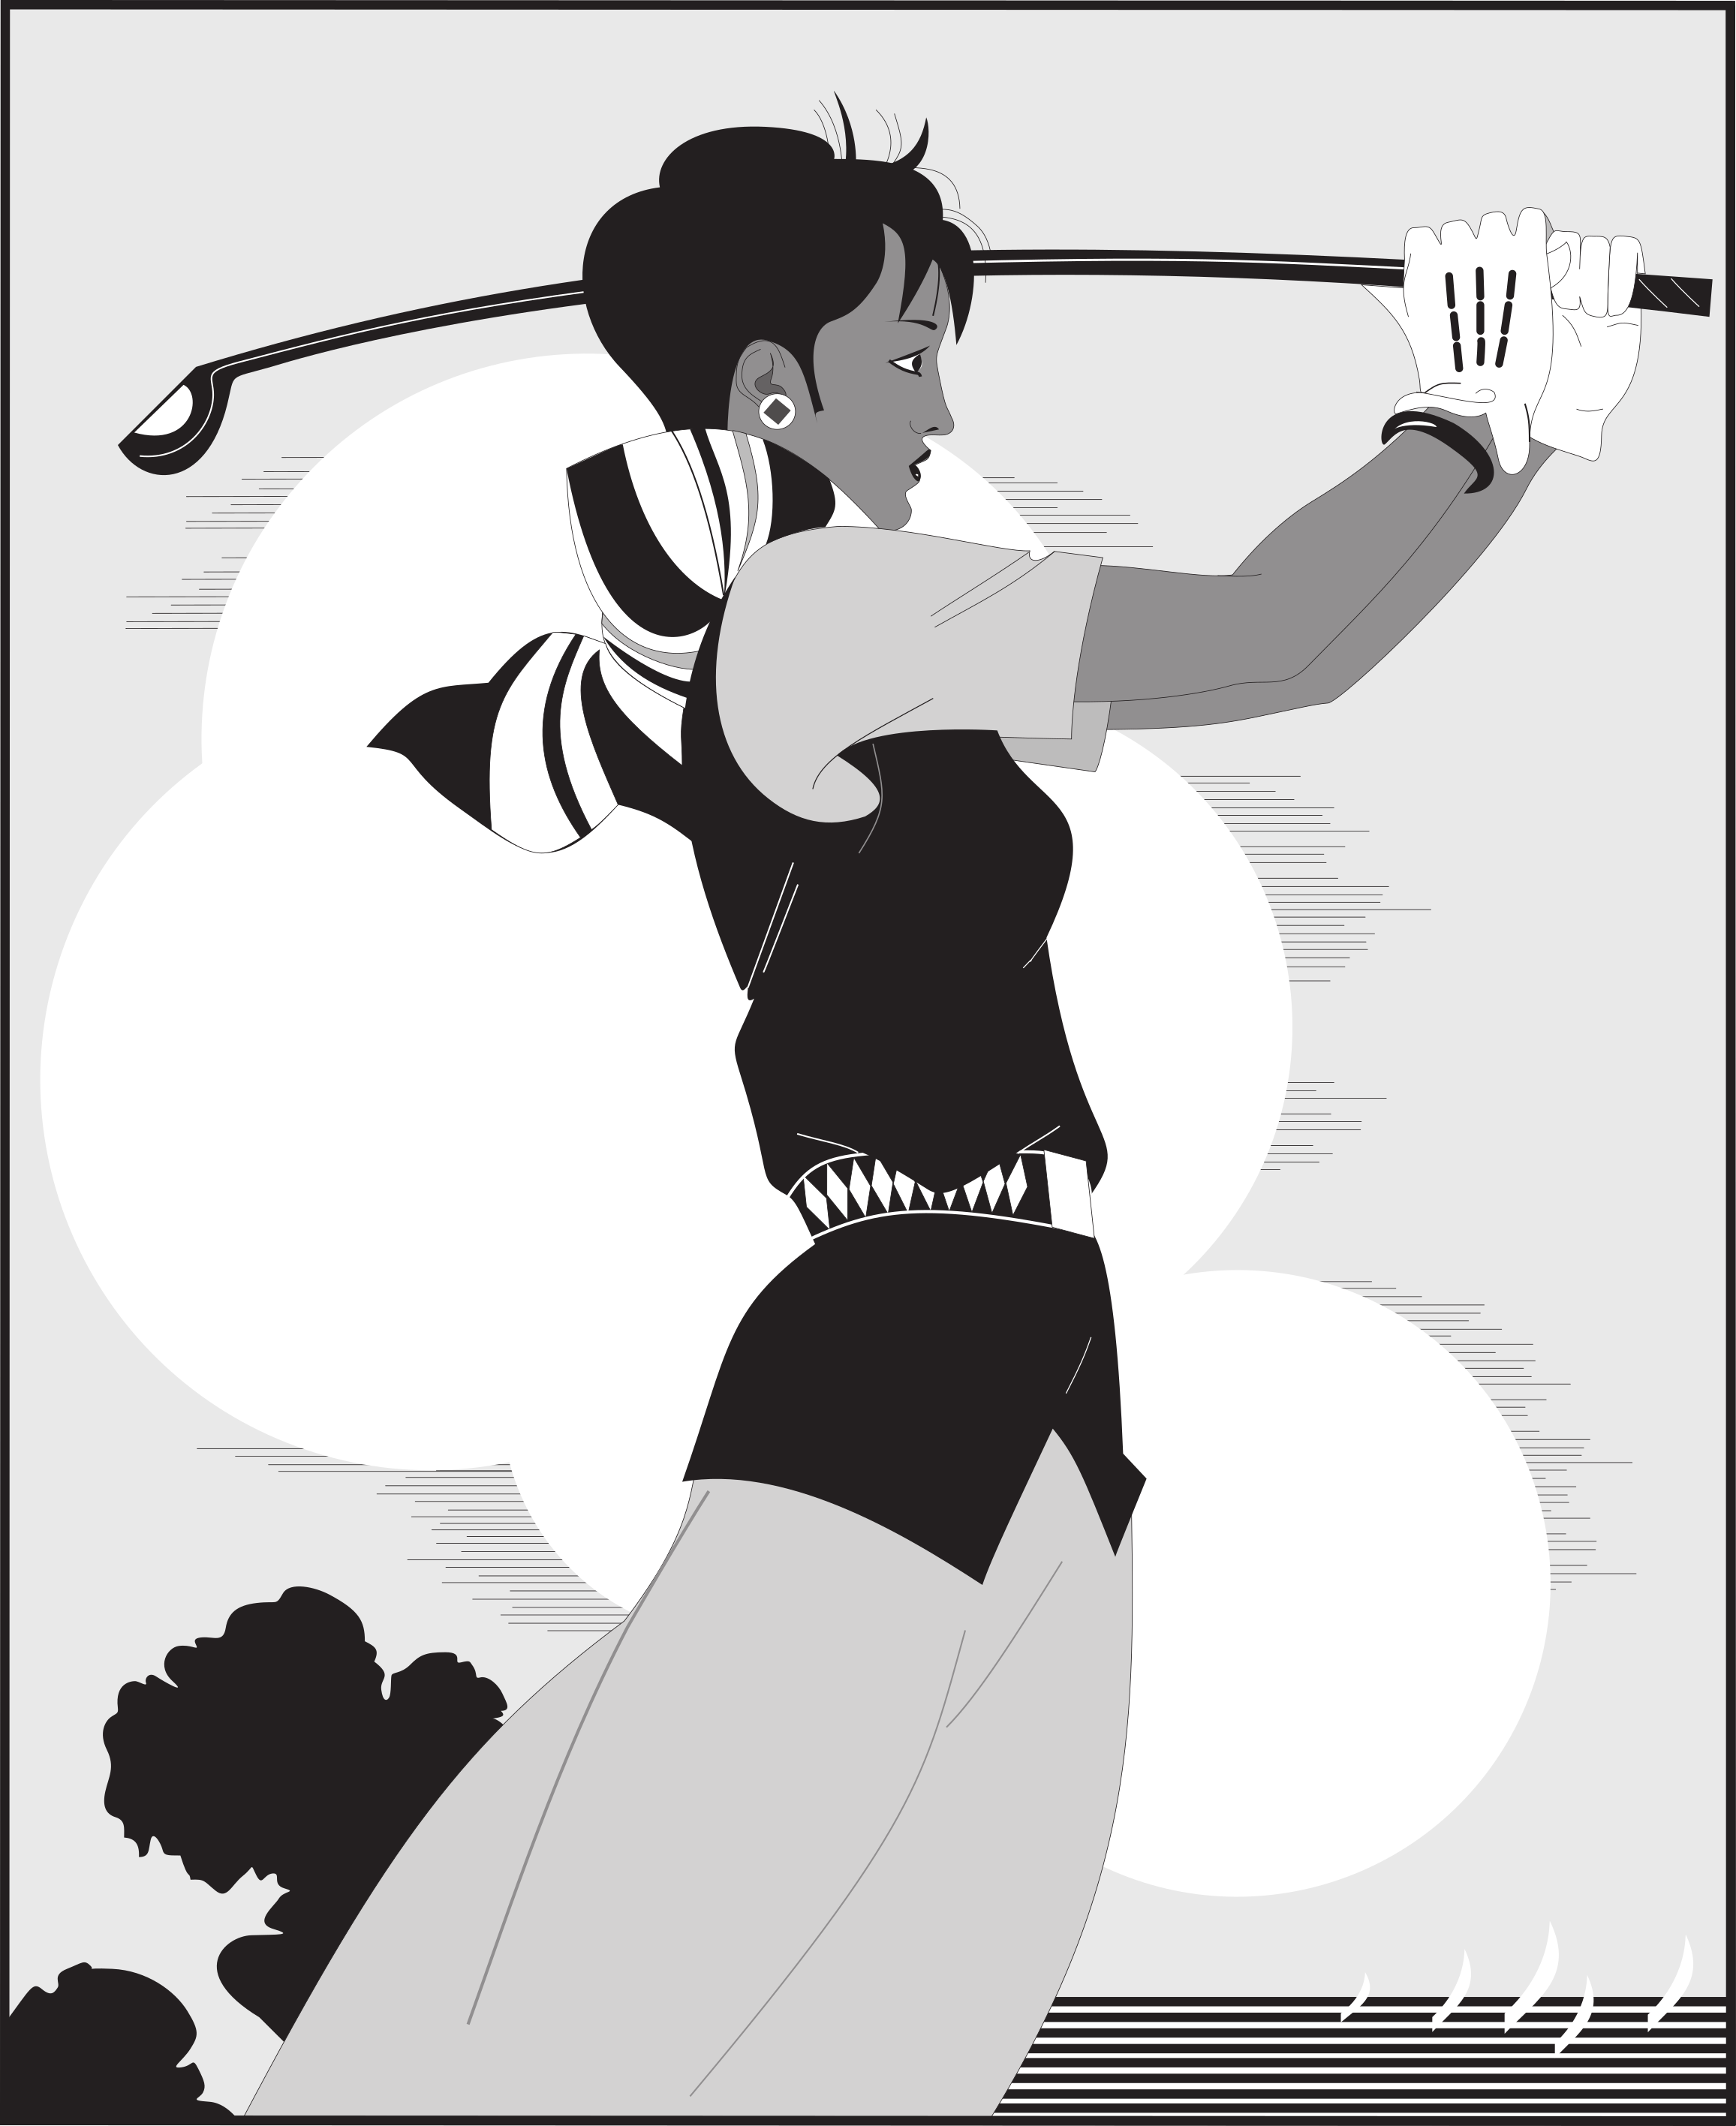
\includegraphics[width=\textwidth]{golfer}
\bicaption[golfer6]{}{打高尔夫球的人}{Fig.$\!$}{The person playing golf}
\end{minipage}
\end{figure}

\subsubsection{子图}[Sub-picture example]
注意:子图题注也可以只用中文。规范规定“分图题置于分图之下或图题之下”,但没有给出具体的格式要求。
没有要求的另外一个说法就是“无论什么格式都不对”。
所以只有在一个图中有标注“a),b)”,无法使用\cs{subfigure}的情况下,使用最后一个图例中的格式设置方法,否则不要使用。
为了应对“无论什么格式都不对”,这个子图图题使用“minipage”和“description”环境,宽度,对齐方式可以按照个人喜好自由设置,是否使用双语子图图题也可以自由设置。

\begin{figure}[!h]
\setlength{\subfigcapskip}{-1bp}
\centering
\begin{minipage}{\textwidth}
\centering
\subfigure{\label{golfer41}}\addtocounter{subfigure}{-2}
\subfigure[The person playing golf]{\subfigure[打高尔夫球的人~1]{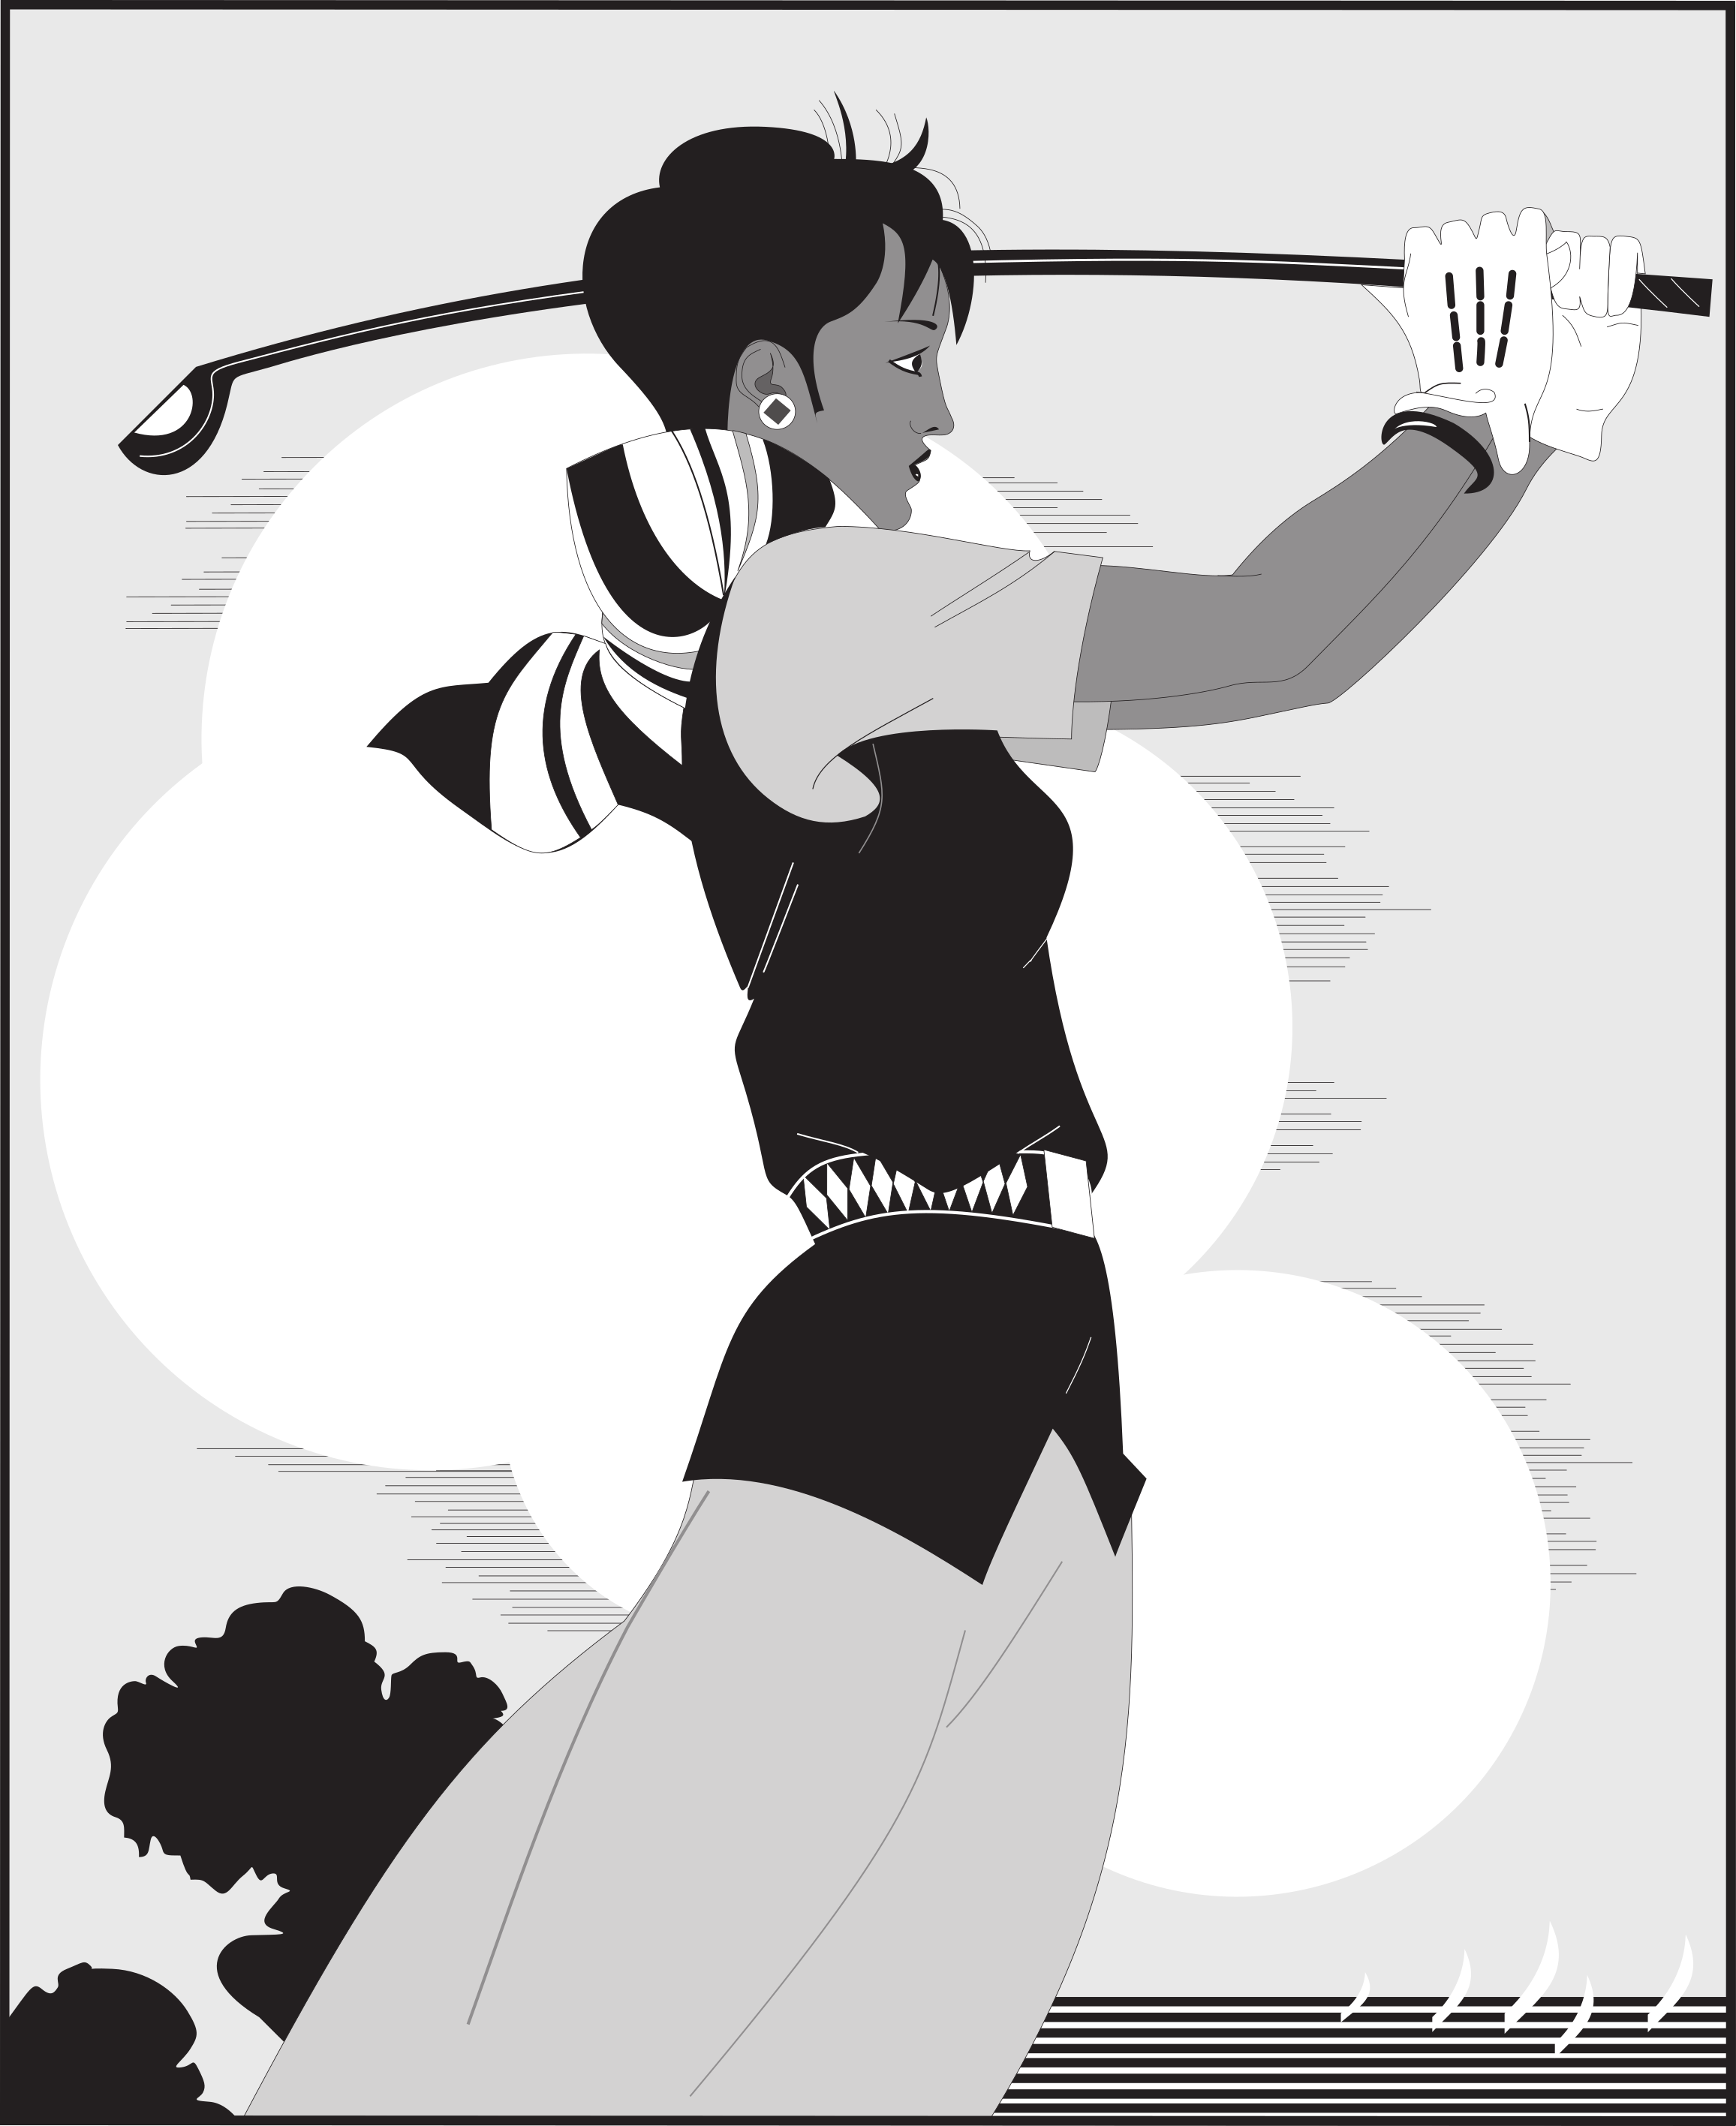
\includegraphics[width=0.4\textwidth]{golfer}}}
\hspace{2em}
\subfigure{\label{golfer42}}\addtocounter{subfigure}{-2}
\subfigure[The person playing golf]{\subfigure[打高尔夫球的人~2]{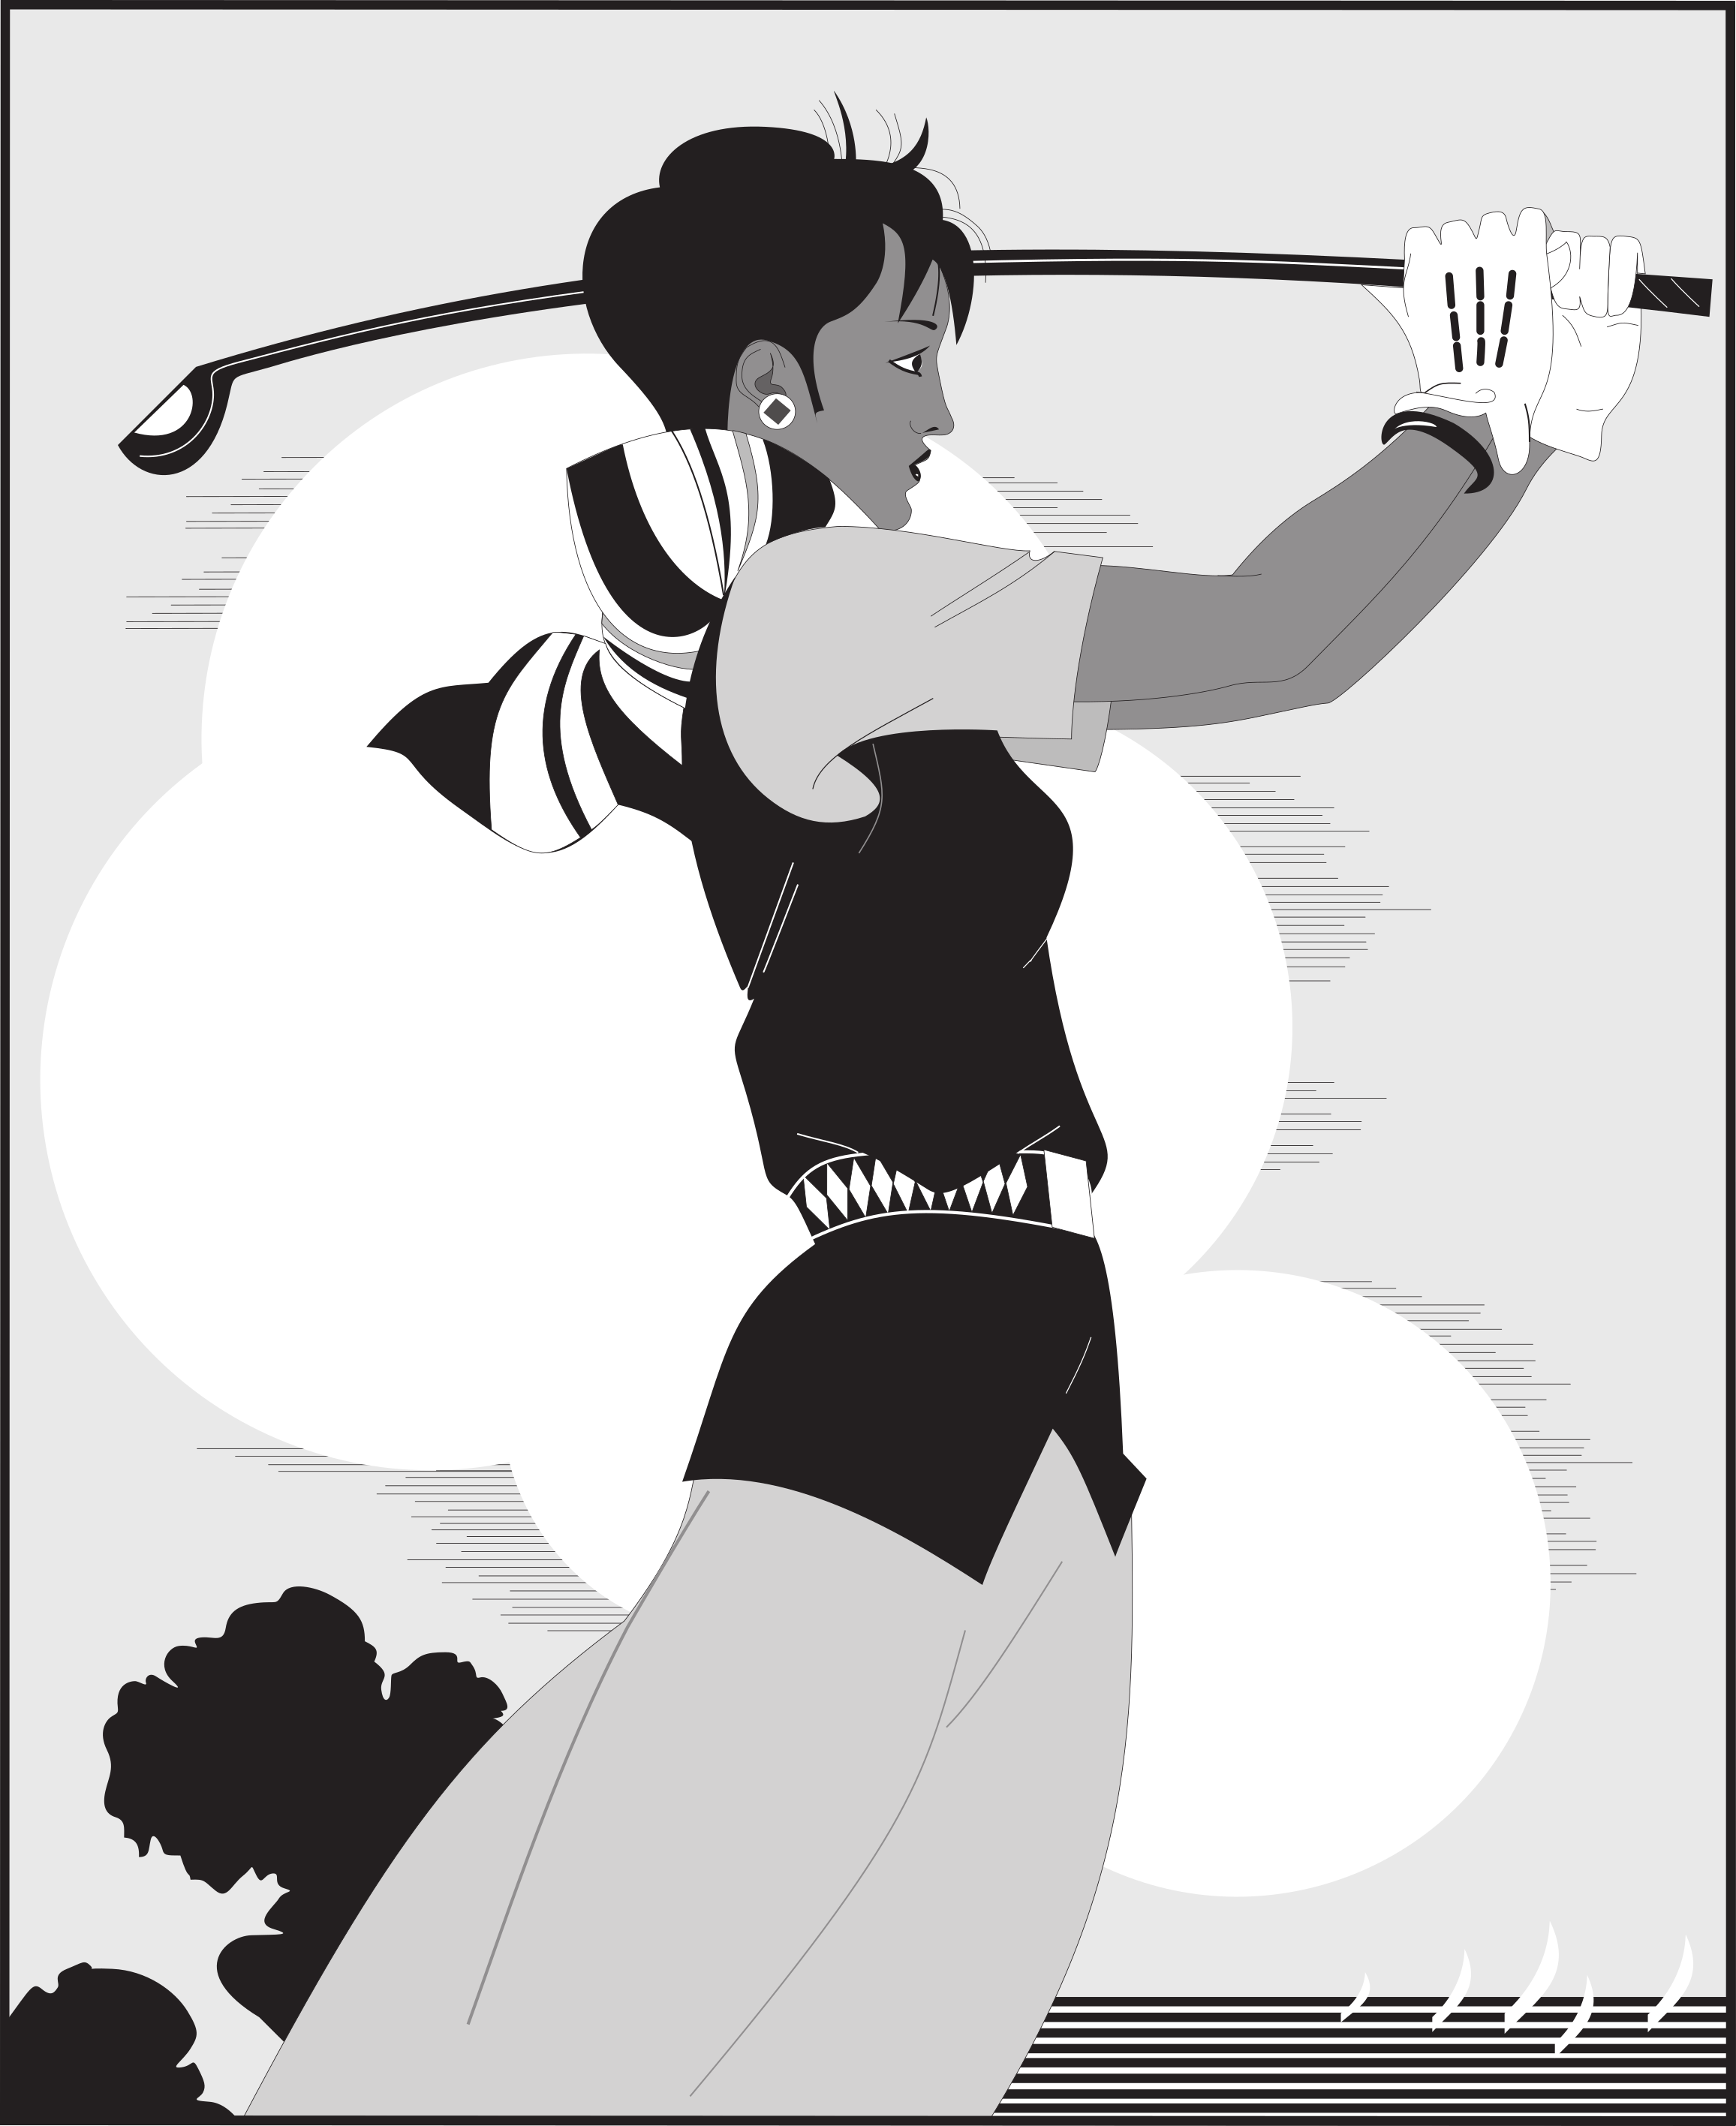
\includegraphics[width=0.4\textwidth]{golfer}}}
\end{minipage}
\centering
\begin{minipage}{\textwidth}
\centering
\subfigure{\label{golfer43}}\addtocounter{subfigure}{-2}
\subfigure[The person playing golf]{\subfigure[打高尔夫球的人~3]{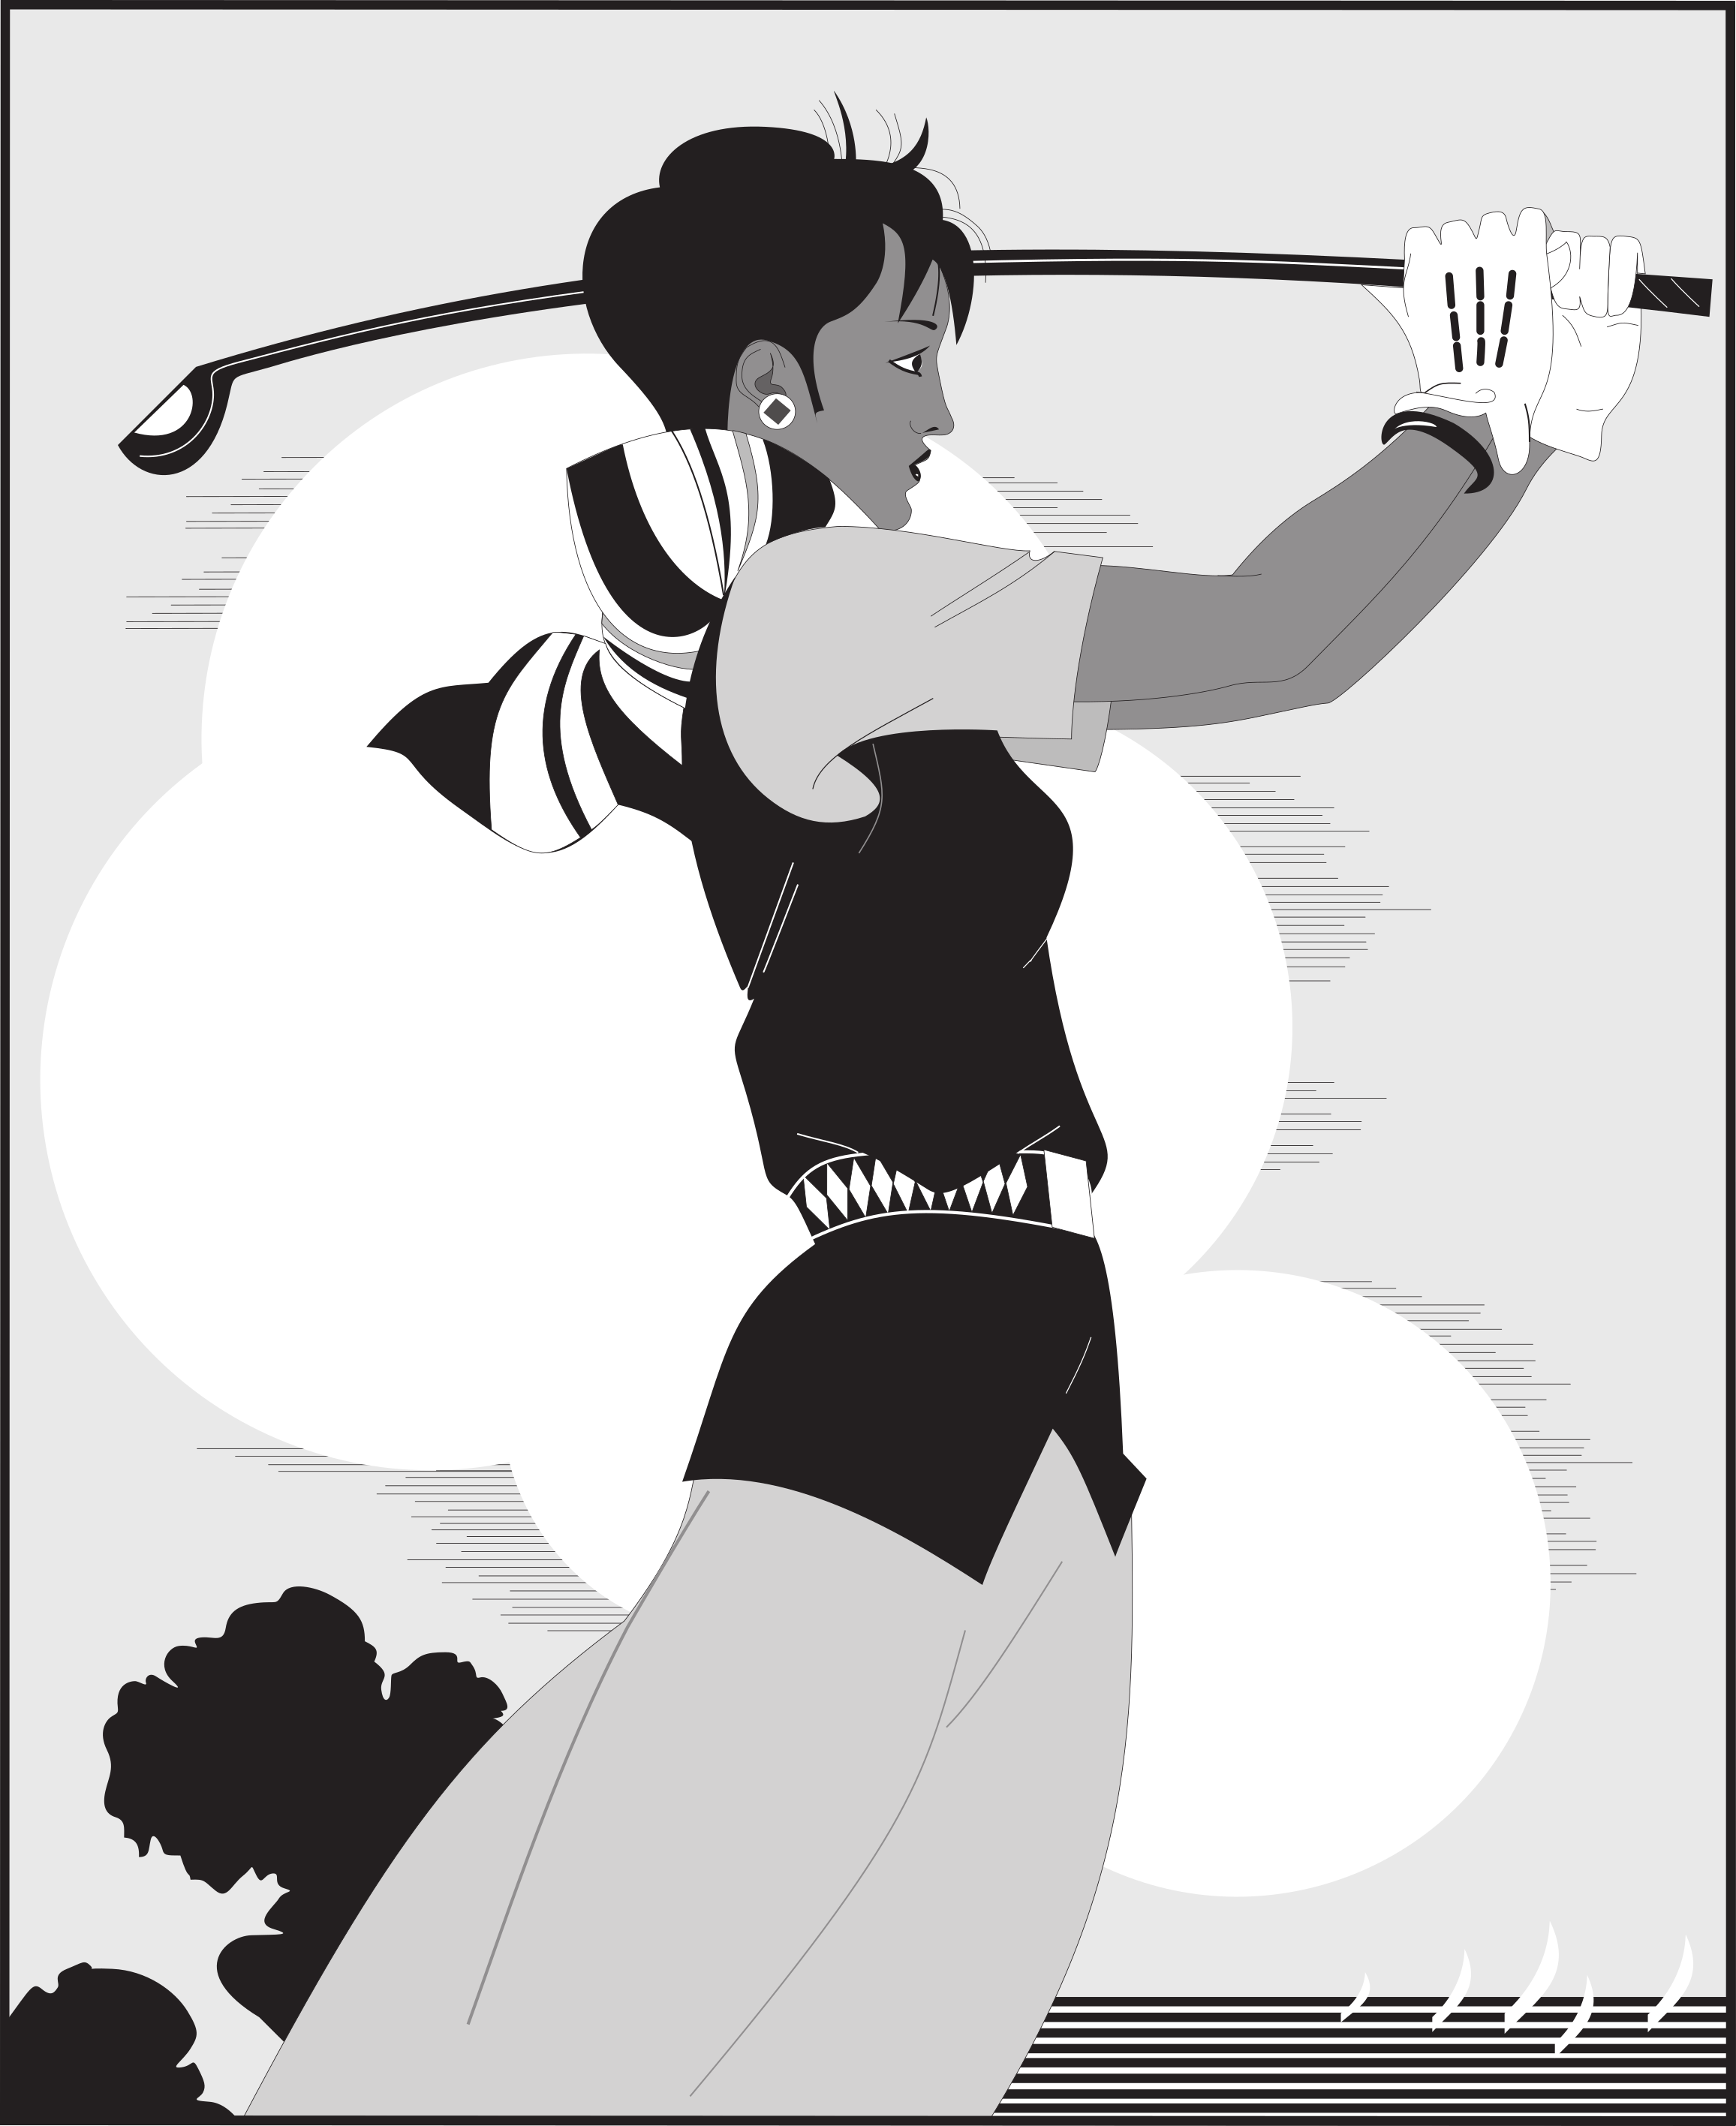
\includegraphics[width=0.4\textwidth]{golfer}}}
\hspace{2em}
\subfigure{\label{golfer44}}\addtocounter{subfigure}{-2}
\subfigure[The person playing golf. Here, 'hang indent' and 'center last line' are not stipulated in the regulation.]{\subfigure[打高尔夫球的人~4。注意,规范中没有明确规定要悬挂缩进、最后一行居中。]{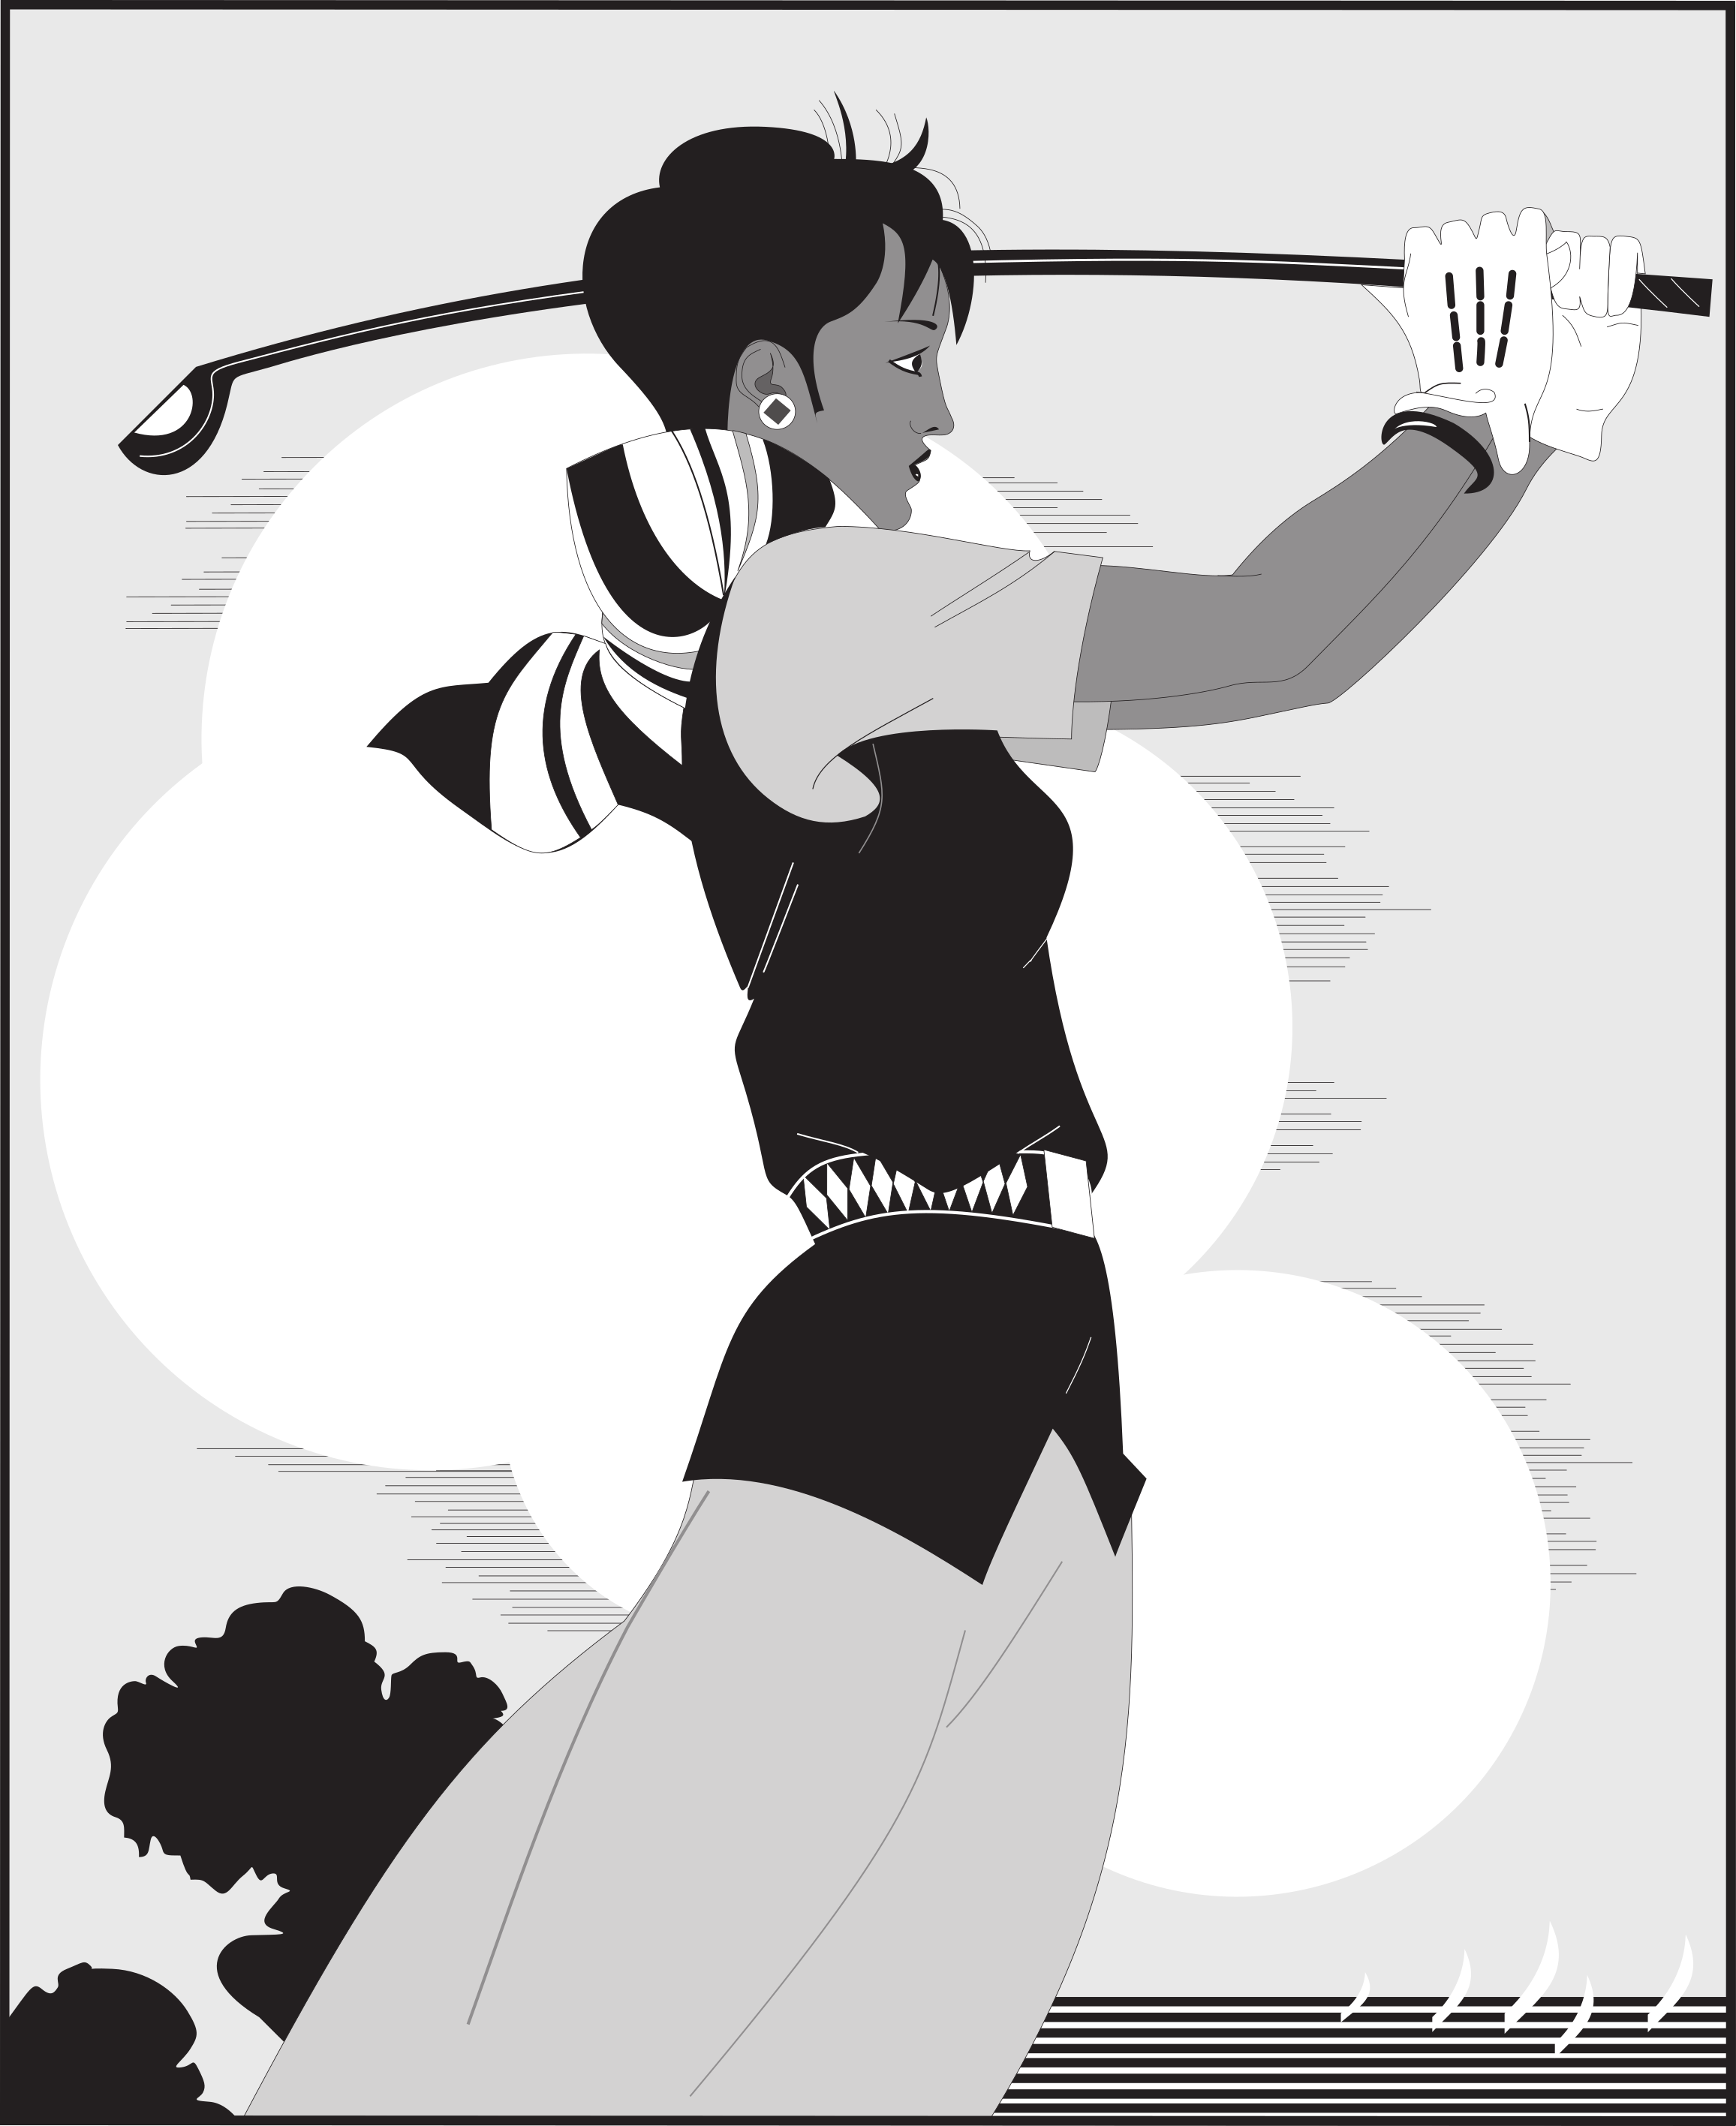
\includegraphics[width=0.4\textwidth]{golfer}}}
\end{minipage}
\vspace{0.2em}
\bicaption[golfer4]{}{打高尔夫球的人}{Fig.$\!$}{The person playing gol}
\end{figure}

\begin{figure}[t]
  \centering
  \begin{minipage}{.7\linewidth}
    \setlength{\subfigcapskip}{-1bp}
    \centering
    \begin{minipage}{\textwidth}
      \centering
      \subfigure{\label{golfer45}}\addtocounter{subfigure}{-2}
      \subfigure[The person playing golf]{\subfigure[打高尔夫球的人~1]{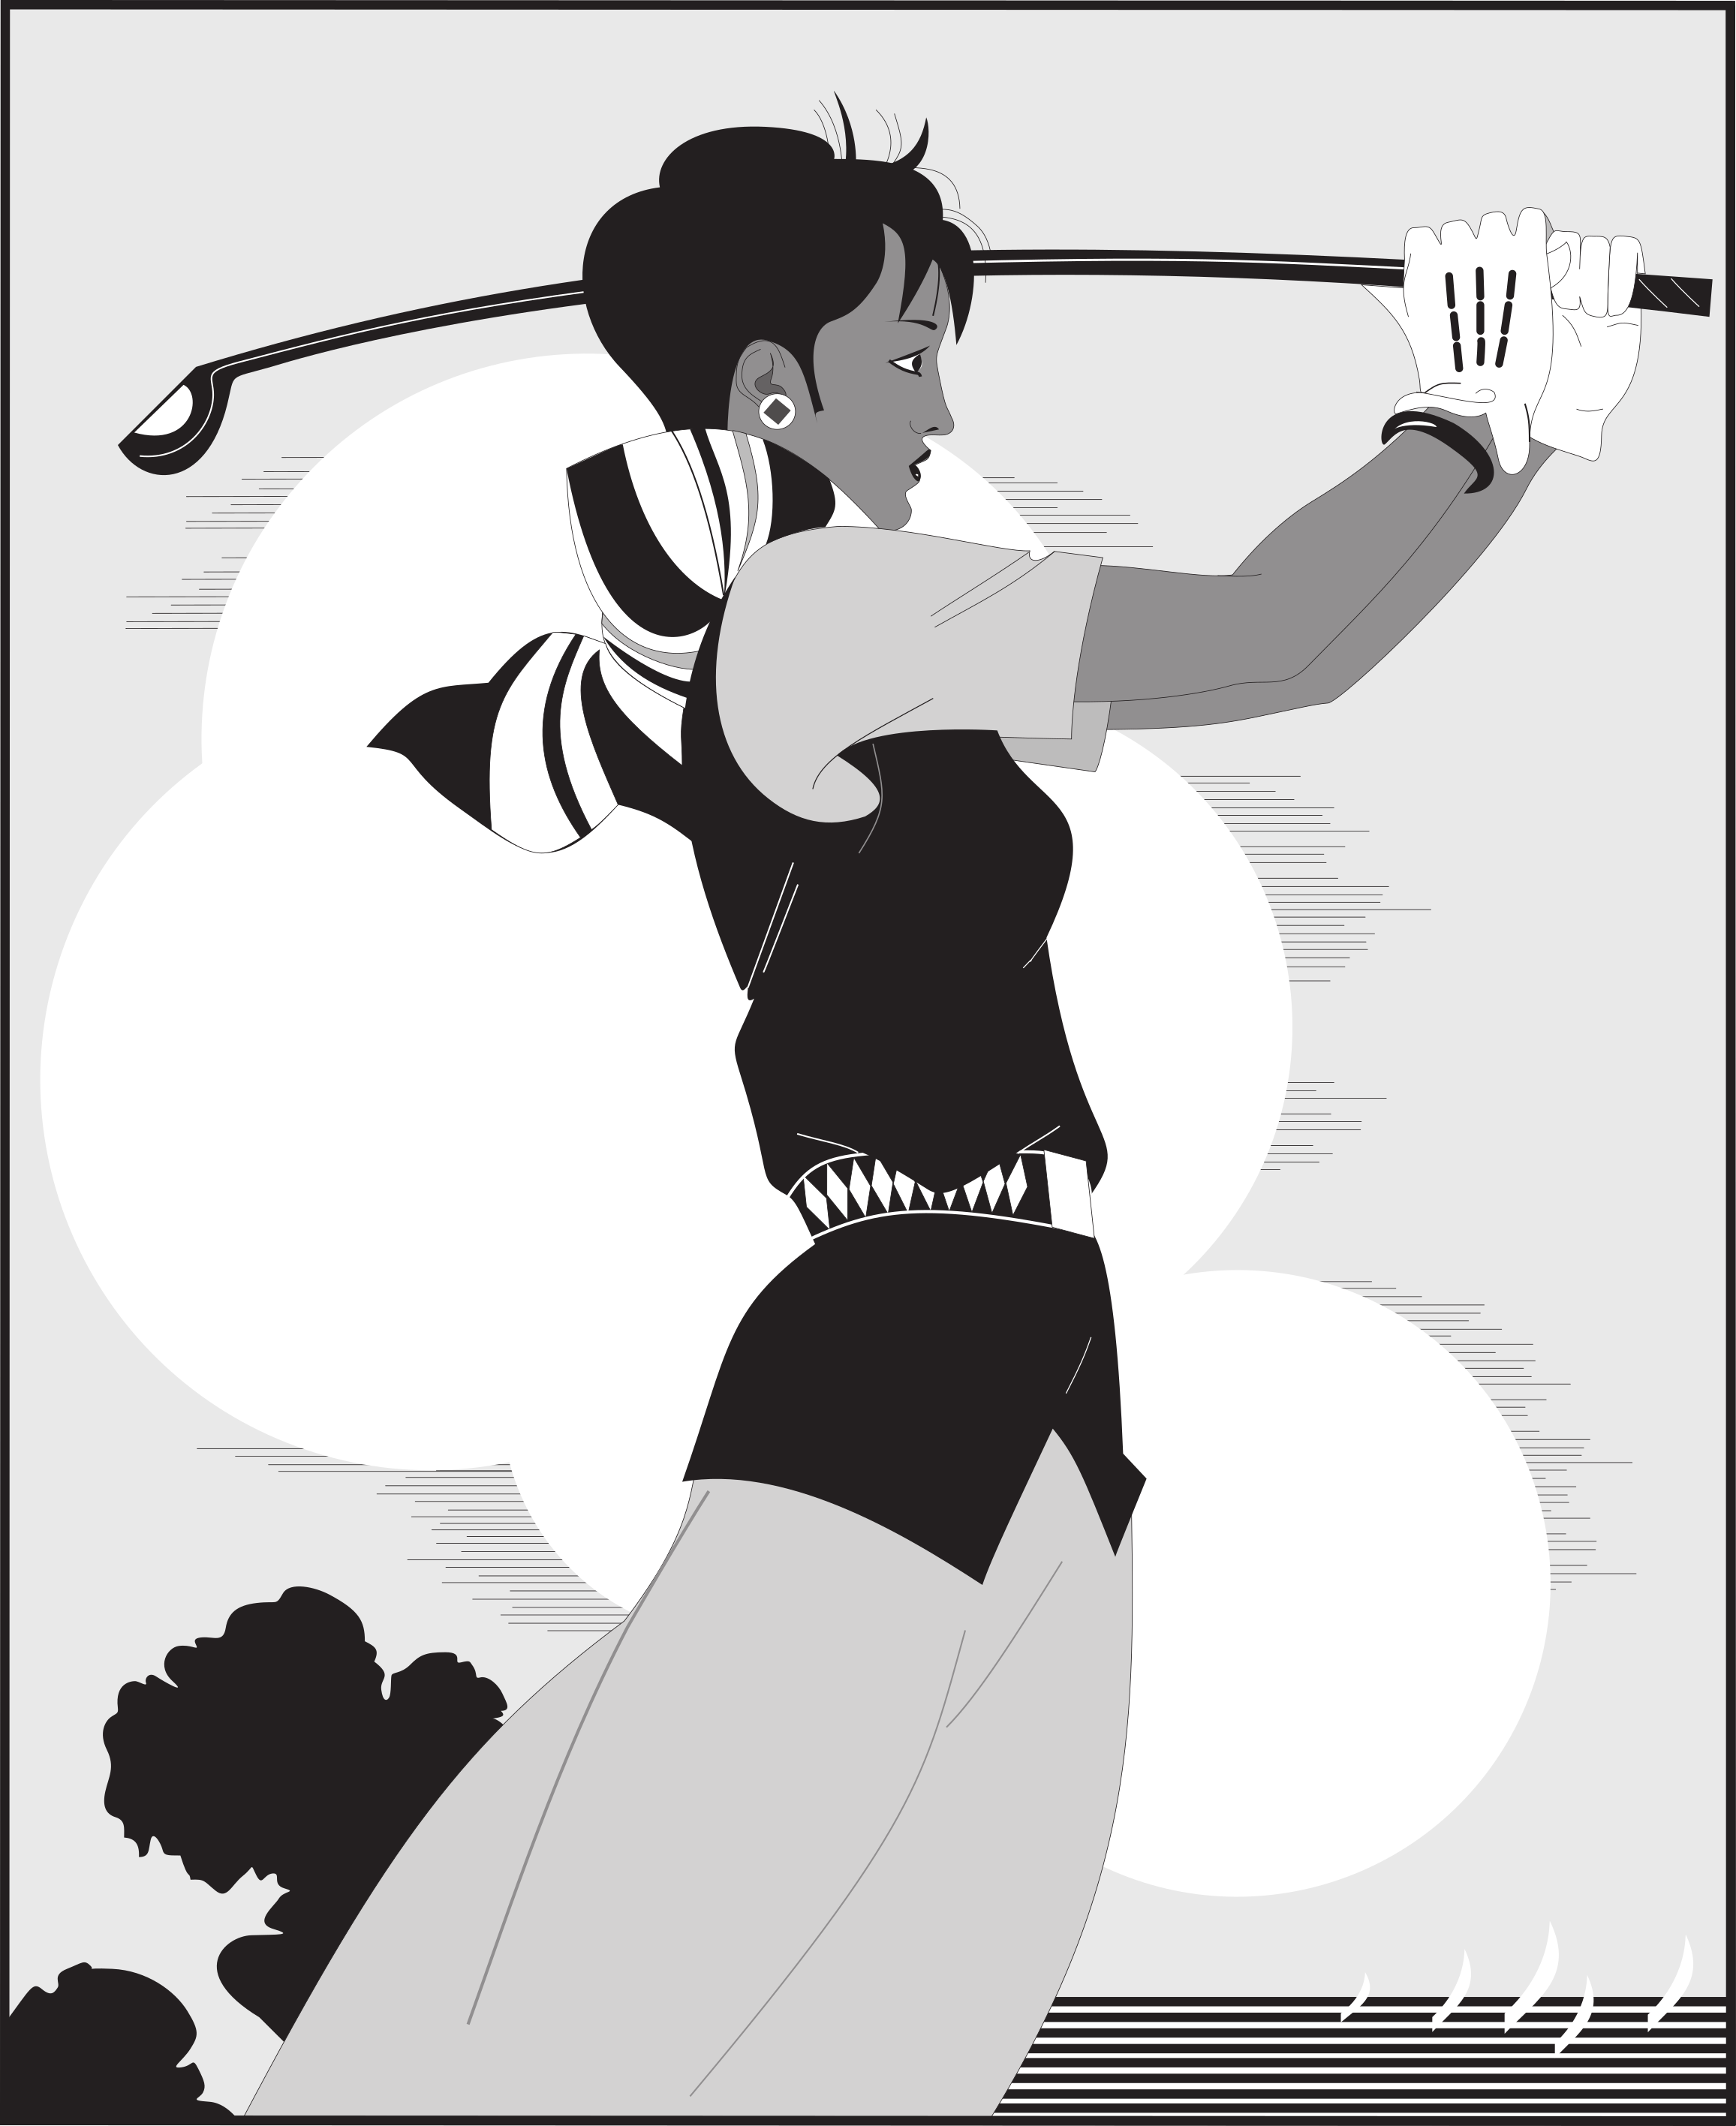
\includegraphics[width=0.4\textwidth]{golfer}}}
      \hspace{4em}
      \subfigure{\label{golfer46}}\addtocounter{subfigure}{-2}
      \subfigure[The person playing golf]{\subfigure[打高尔夫球的人~2]{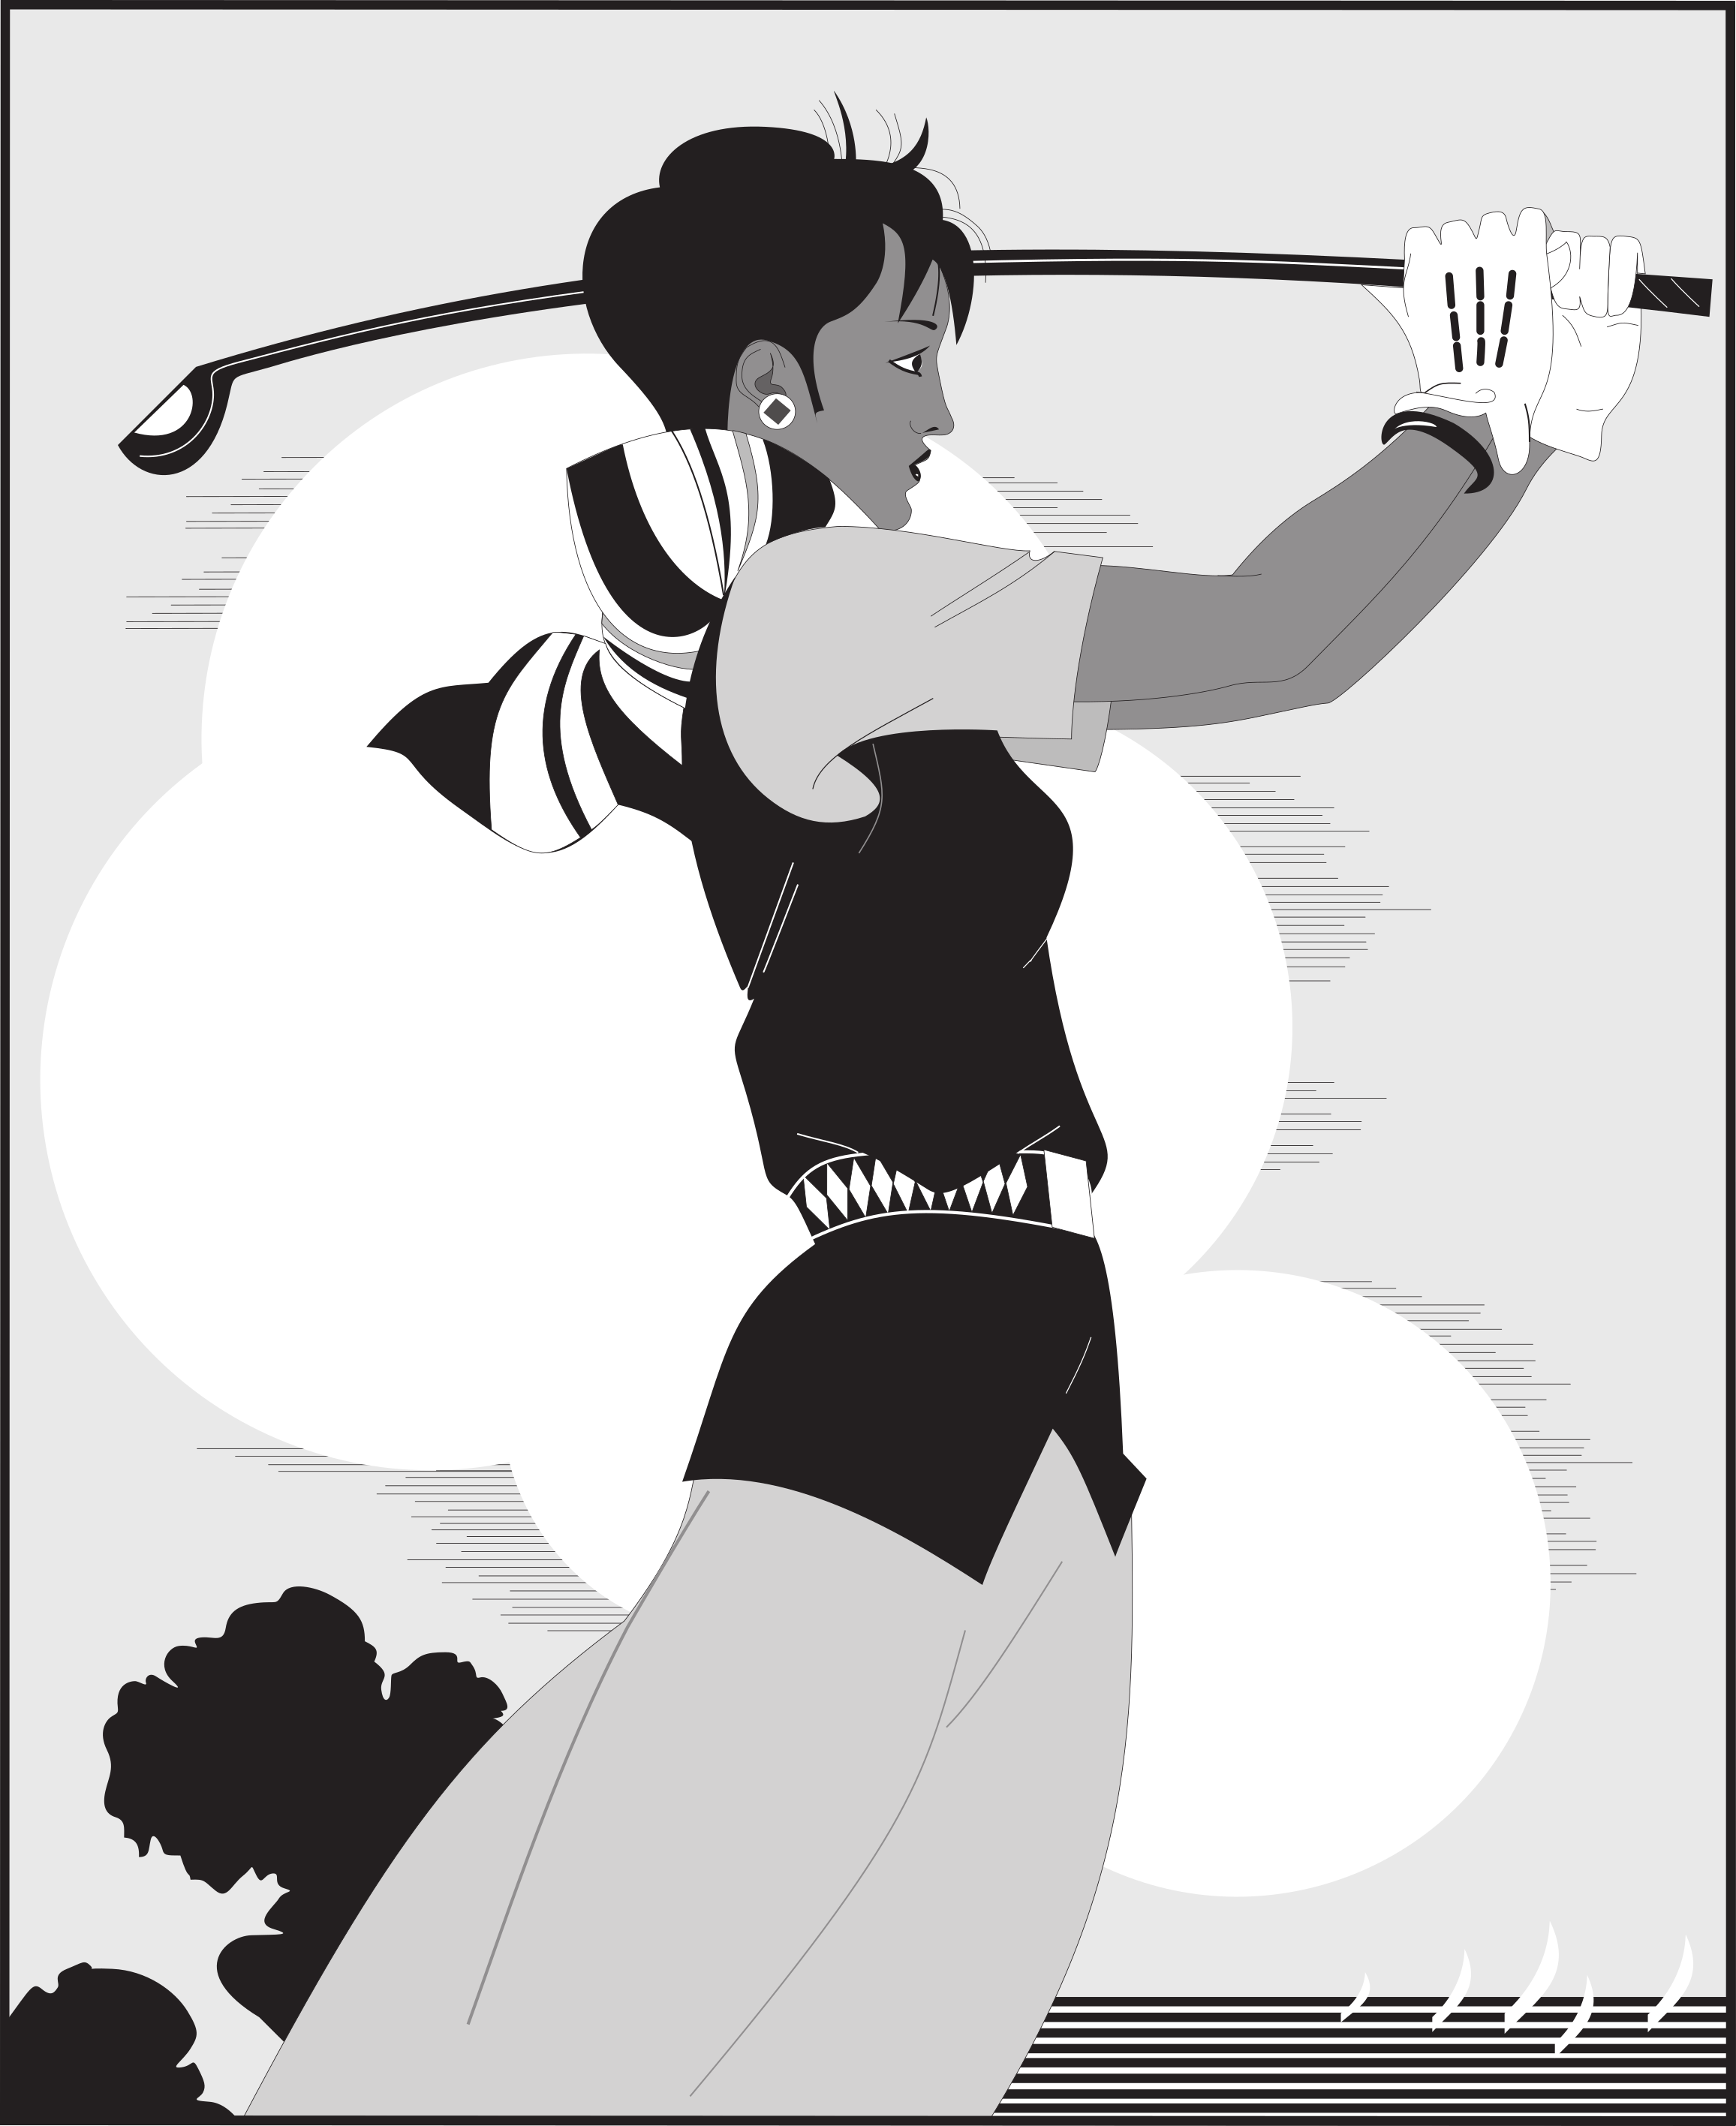
\includegraphics[width=0.4\textwidth]{golfer}}}
    \end{minipage}
    \vskip 0.2em
  \wuhao 注意:这里是中文图注添加位置(我工要求,图注在图题之上)。
    \vspace{0.2em}
\bicaption[golfer47]{}{打高尔夫球的人。注意,此处我工有另外一处要求,子图图题可以位于主图题之下。但由于没有明确说明位于下方具体是什么格式,所以这里不给出举例。}{Fig.$\!$}{The person playing golf. Please note that, although it is appropriate to put subfigures' captions under this caption as stipulated in regulation, but its format is not clearly stated.}
  \end{minipage}
\end{figure}

\begin{figure}[t]
\centering
\begin{tikzpicture}
	\node[anchor=south west,inner sep=0] (image) at (0,0) {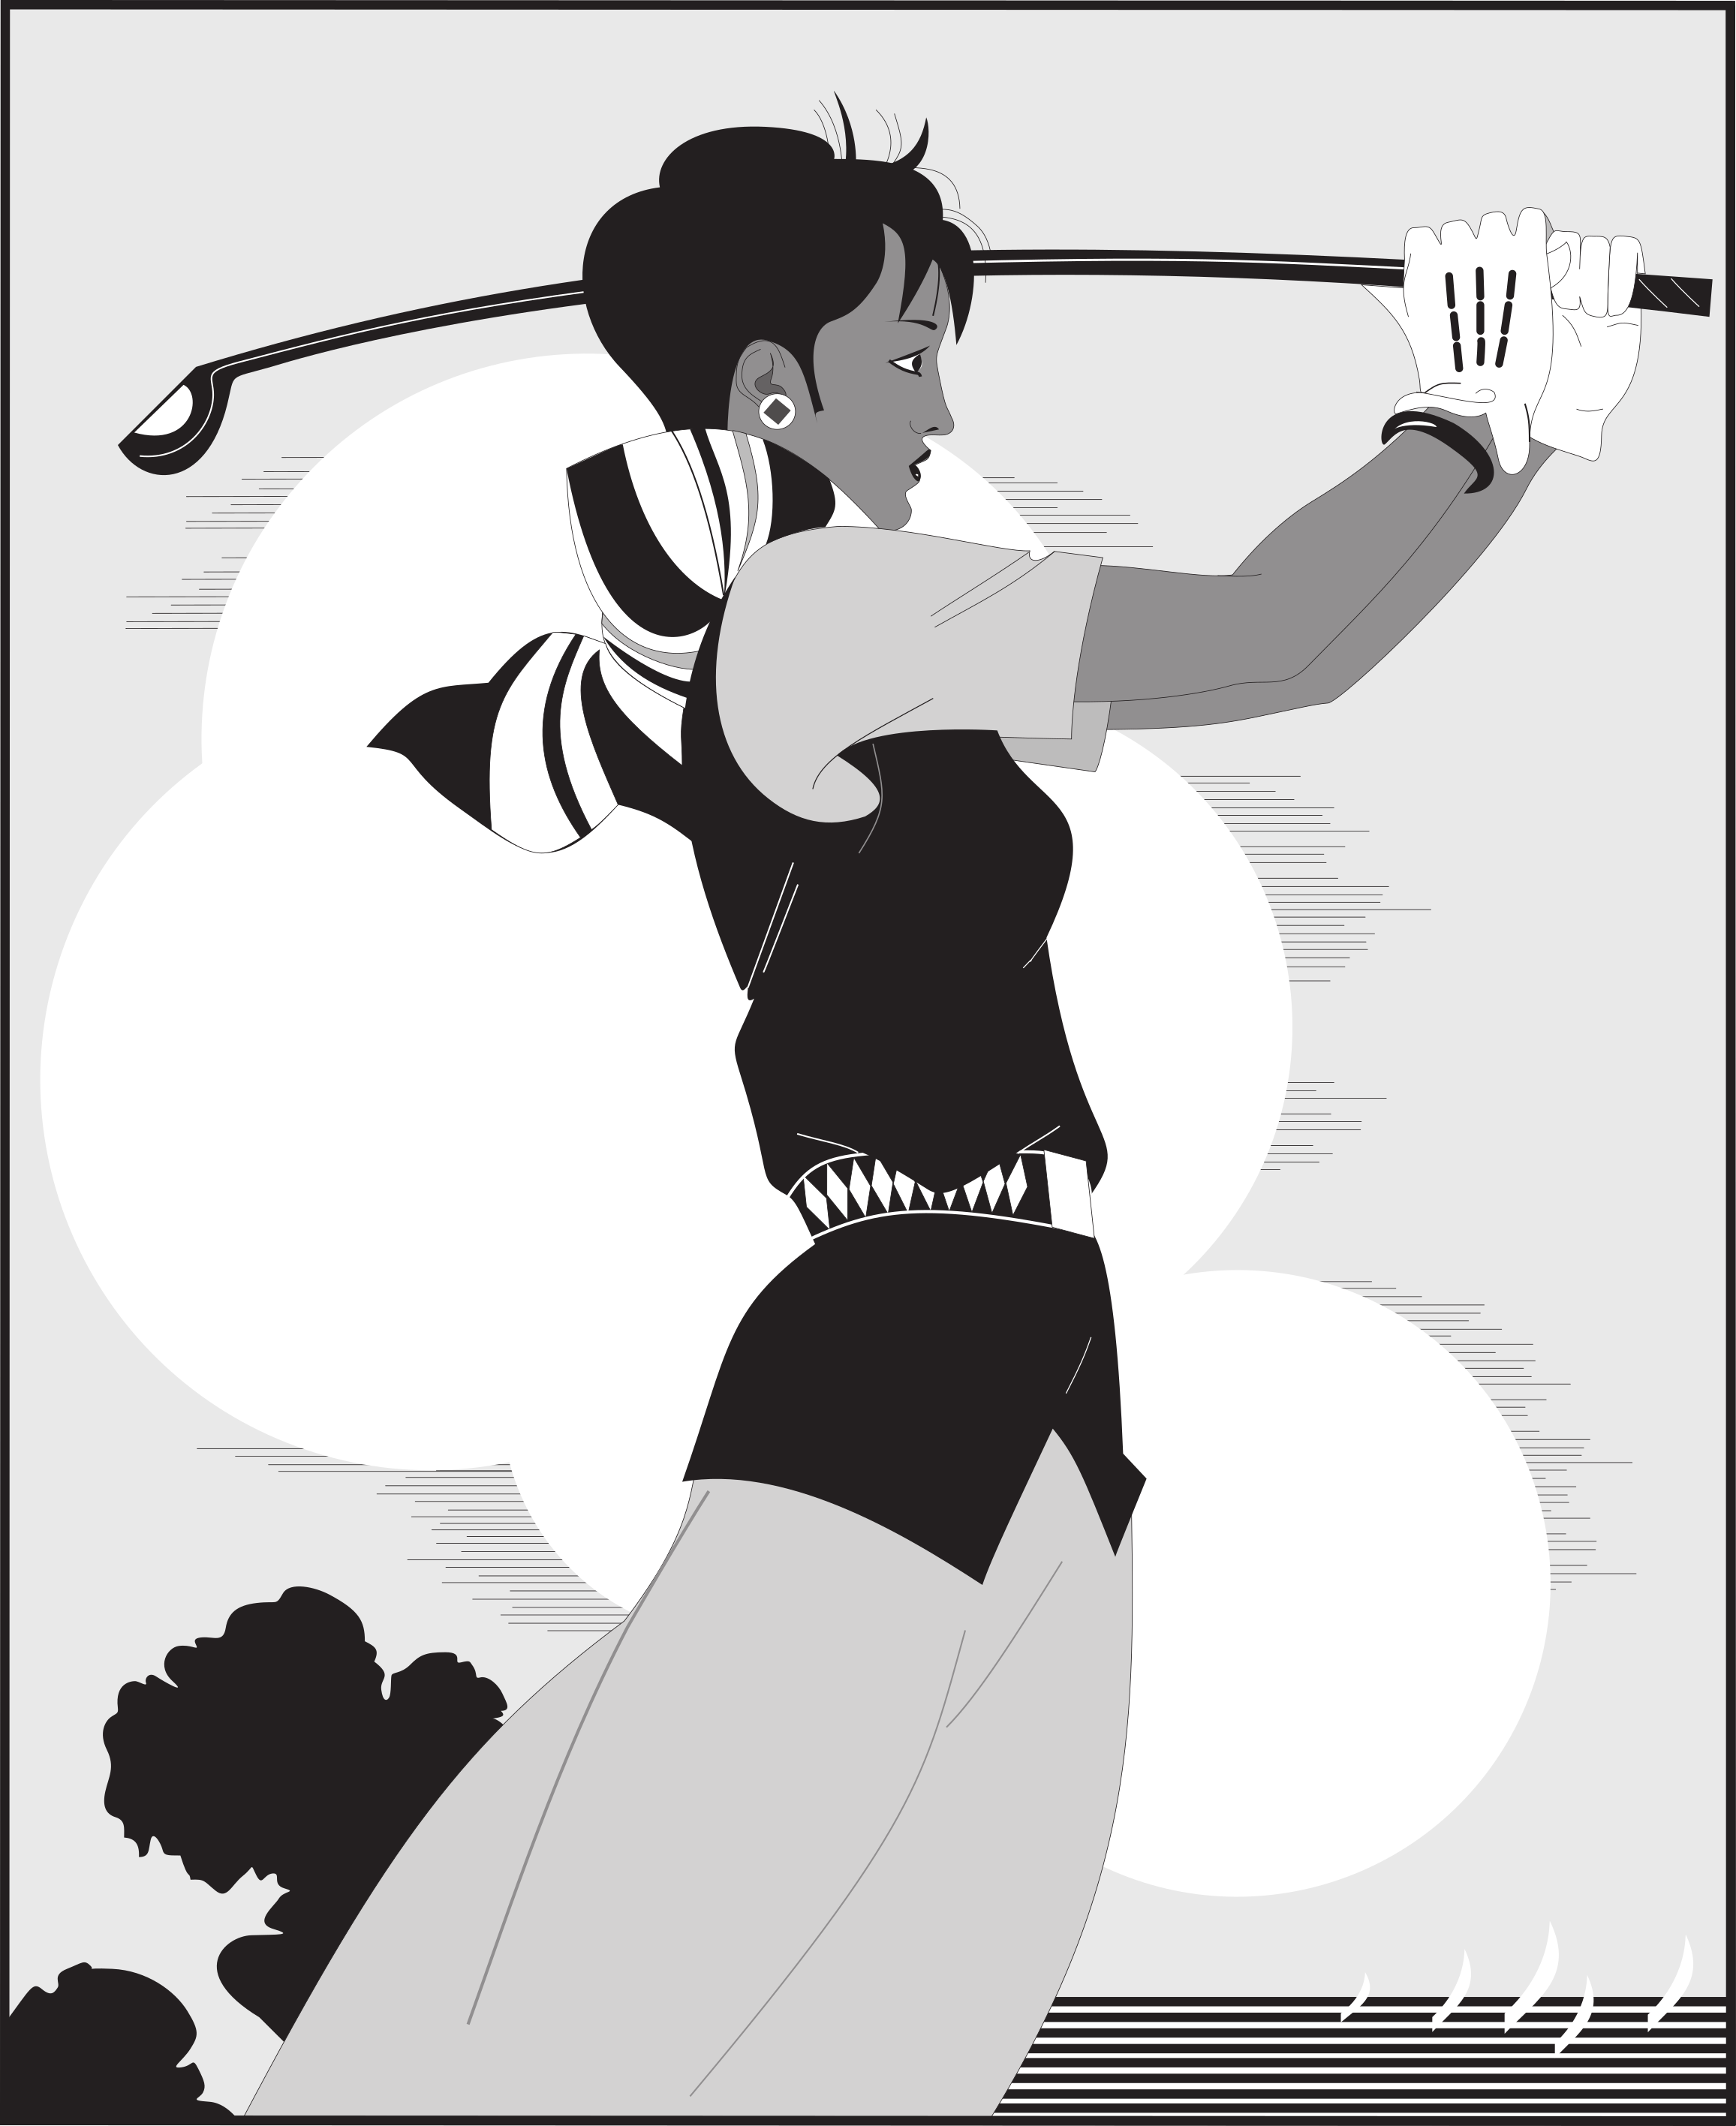
\includegraphics[width=0.3\textwidth]{golfer}};
	\begin{scope}[x={(image.south east)},y={(image.north west)}]
		\node at (0.3,0.5) {a)};
		\node at (0.8,0.2) {b)};
	\end{scope}
\end{tikzpicture}
\bicaption[golfer0]{}{打高尔夫球球的人(博士论文双语题注)}{Fig.$\!$}{The person playing golf (Doctoral thesis)}
\vskip -0.4em
 \hspace{2em}
\begin{minipage}[t]{0.3\textwidth}
\wuhao \setlist[description]{font=\normalfont}
	\begin{description}
		\item[a)]子图图题
	\end{description}
 \end{minipage}
 \hspace{2em}
 \begin{minipage}[t]{0.3\textwidth}
\wuhao \setlist[description]{font=\normalfont}
	\begin{description}
		\item[b)]子图图题
		\item[b)]Subfigure caption
	\end{description}
\end{minipage}
\end{figure}


\begin{figure}[!h]
	\centering
	\begin{sideways}
		\begin{minipage}{\textheight}
			\centering
			\fbox{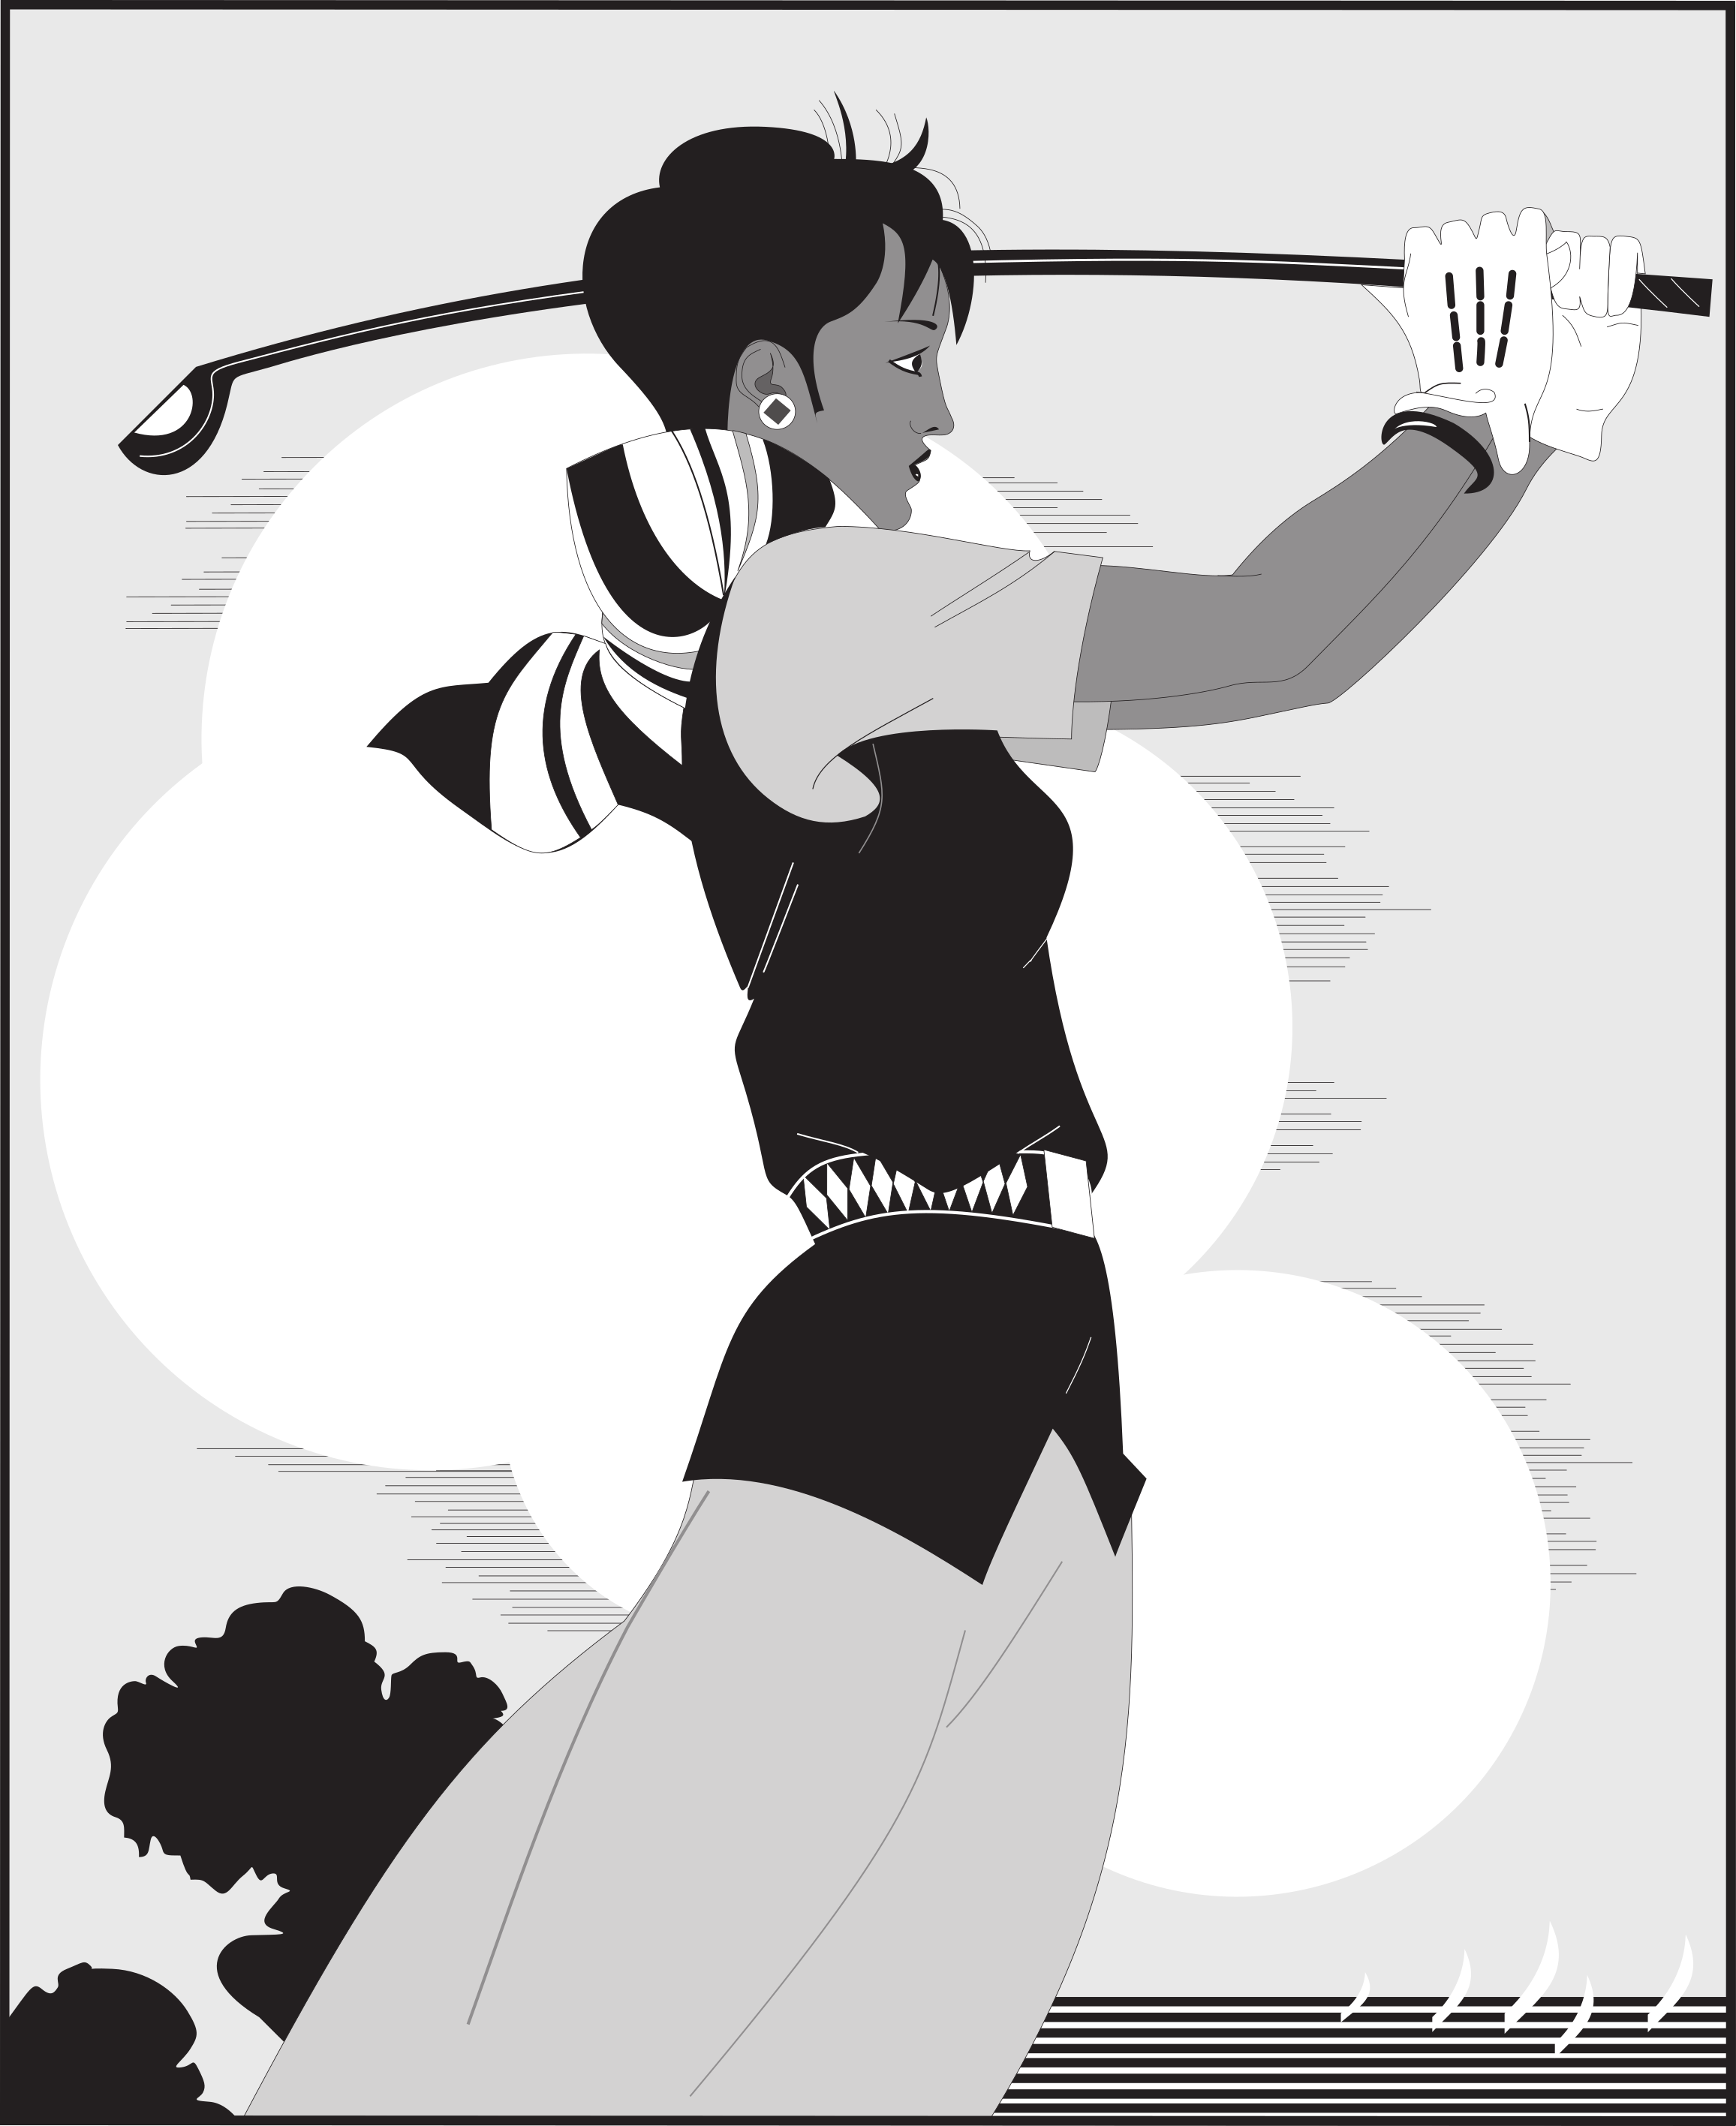
\includegraphics[width=0.2\textwidth]{golfer}}
			\fbox{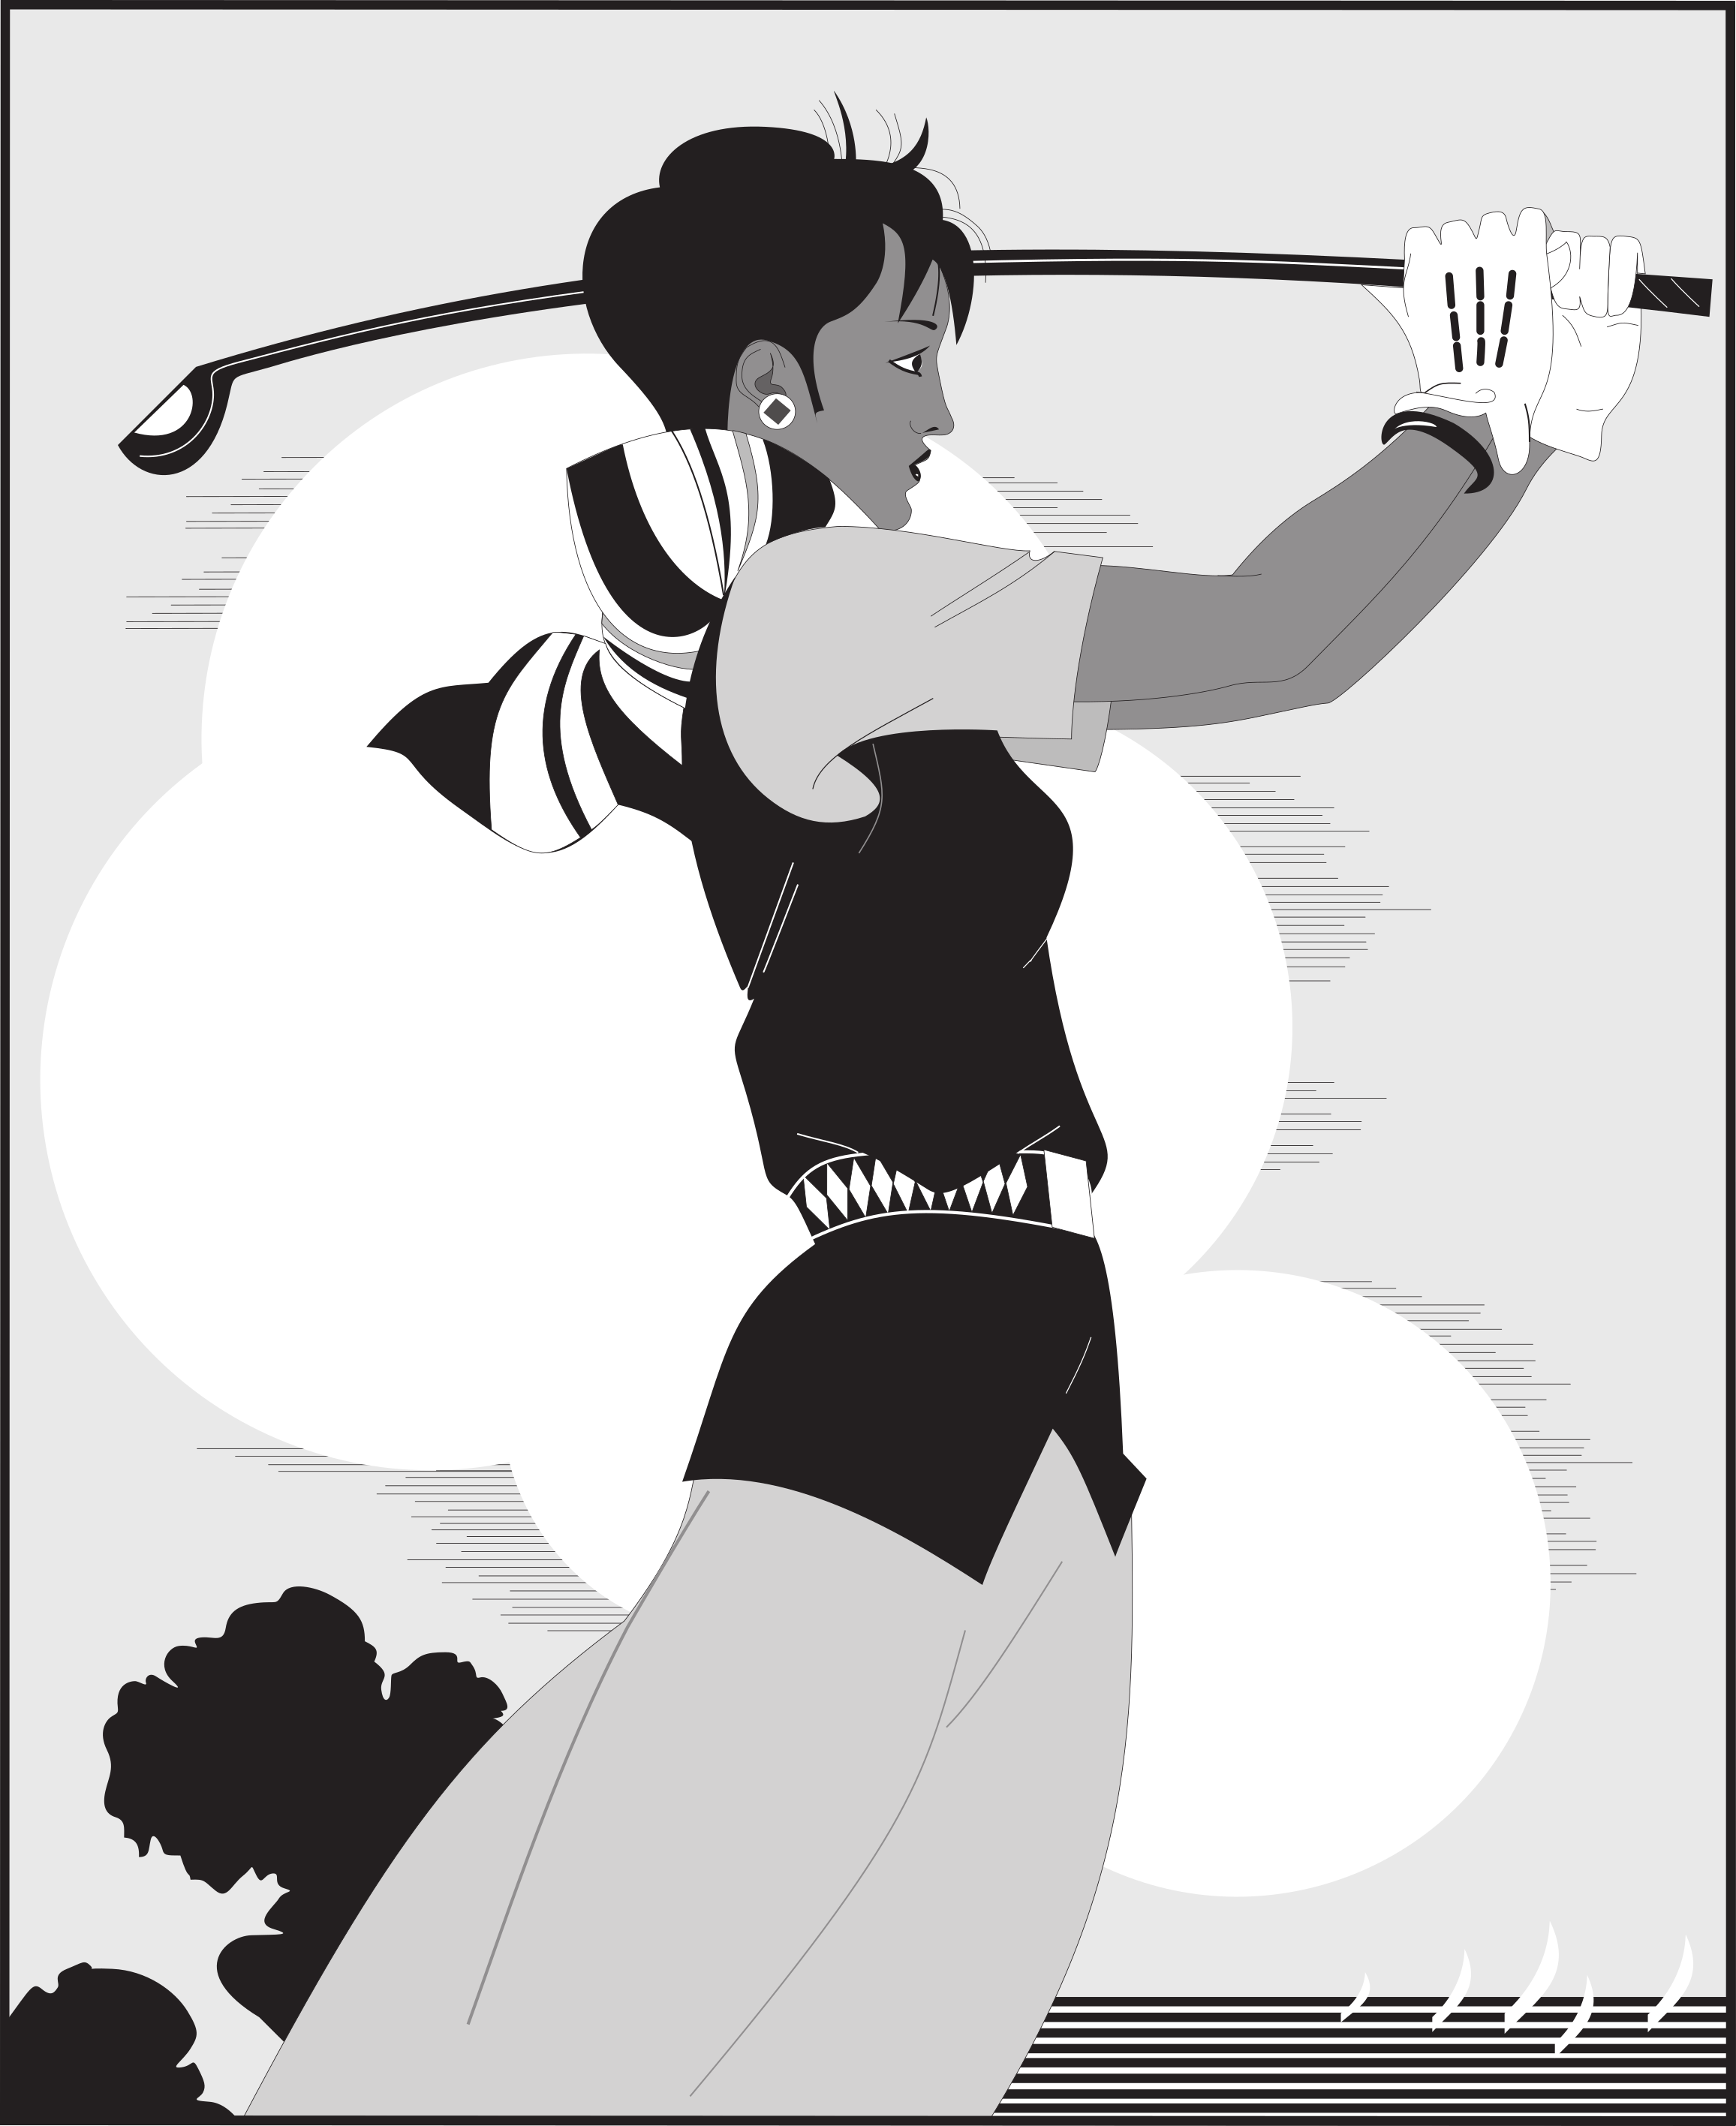
\includegraphics[width=0.2\textwidth]{golfer}}
			\fbox{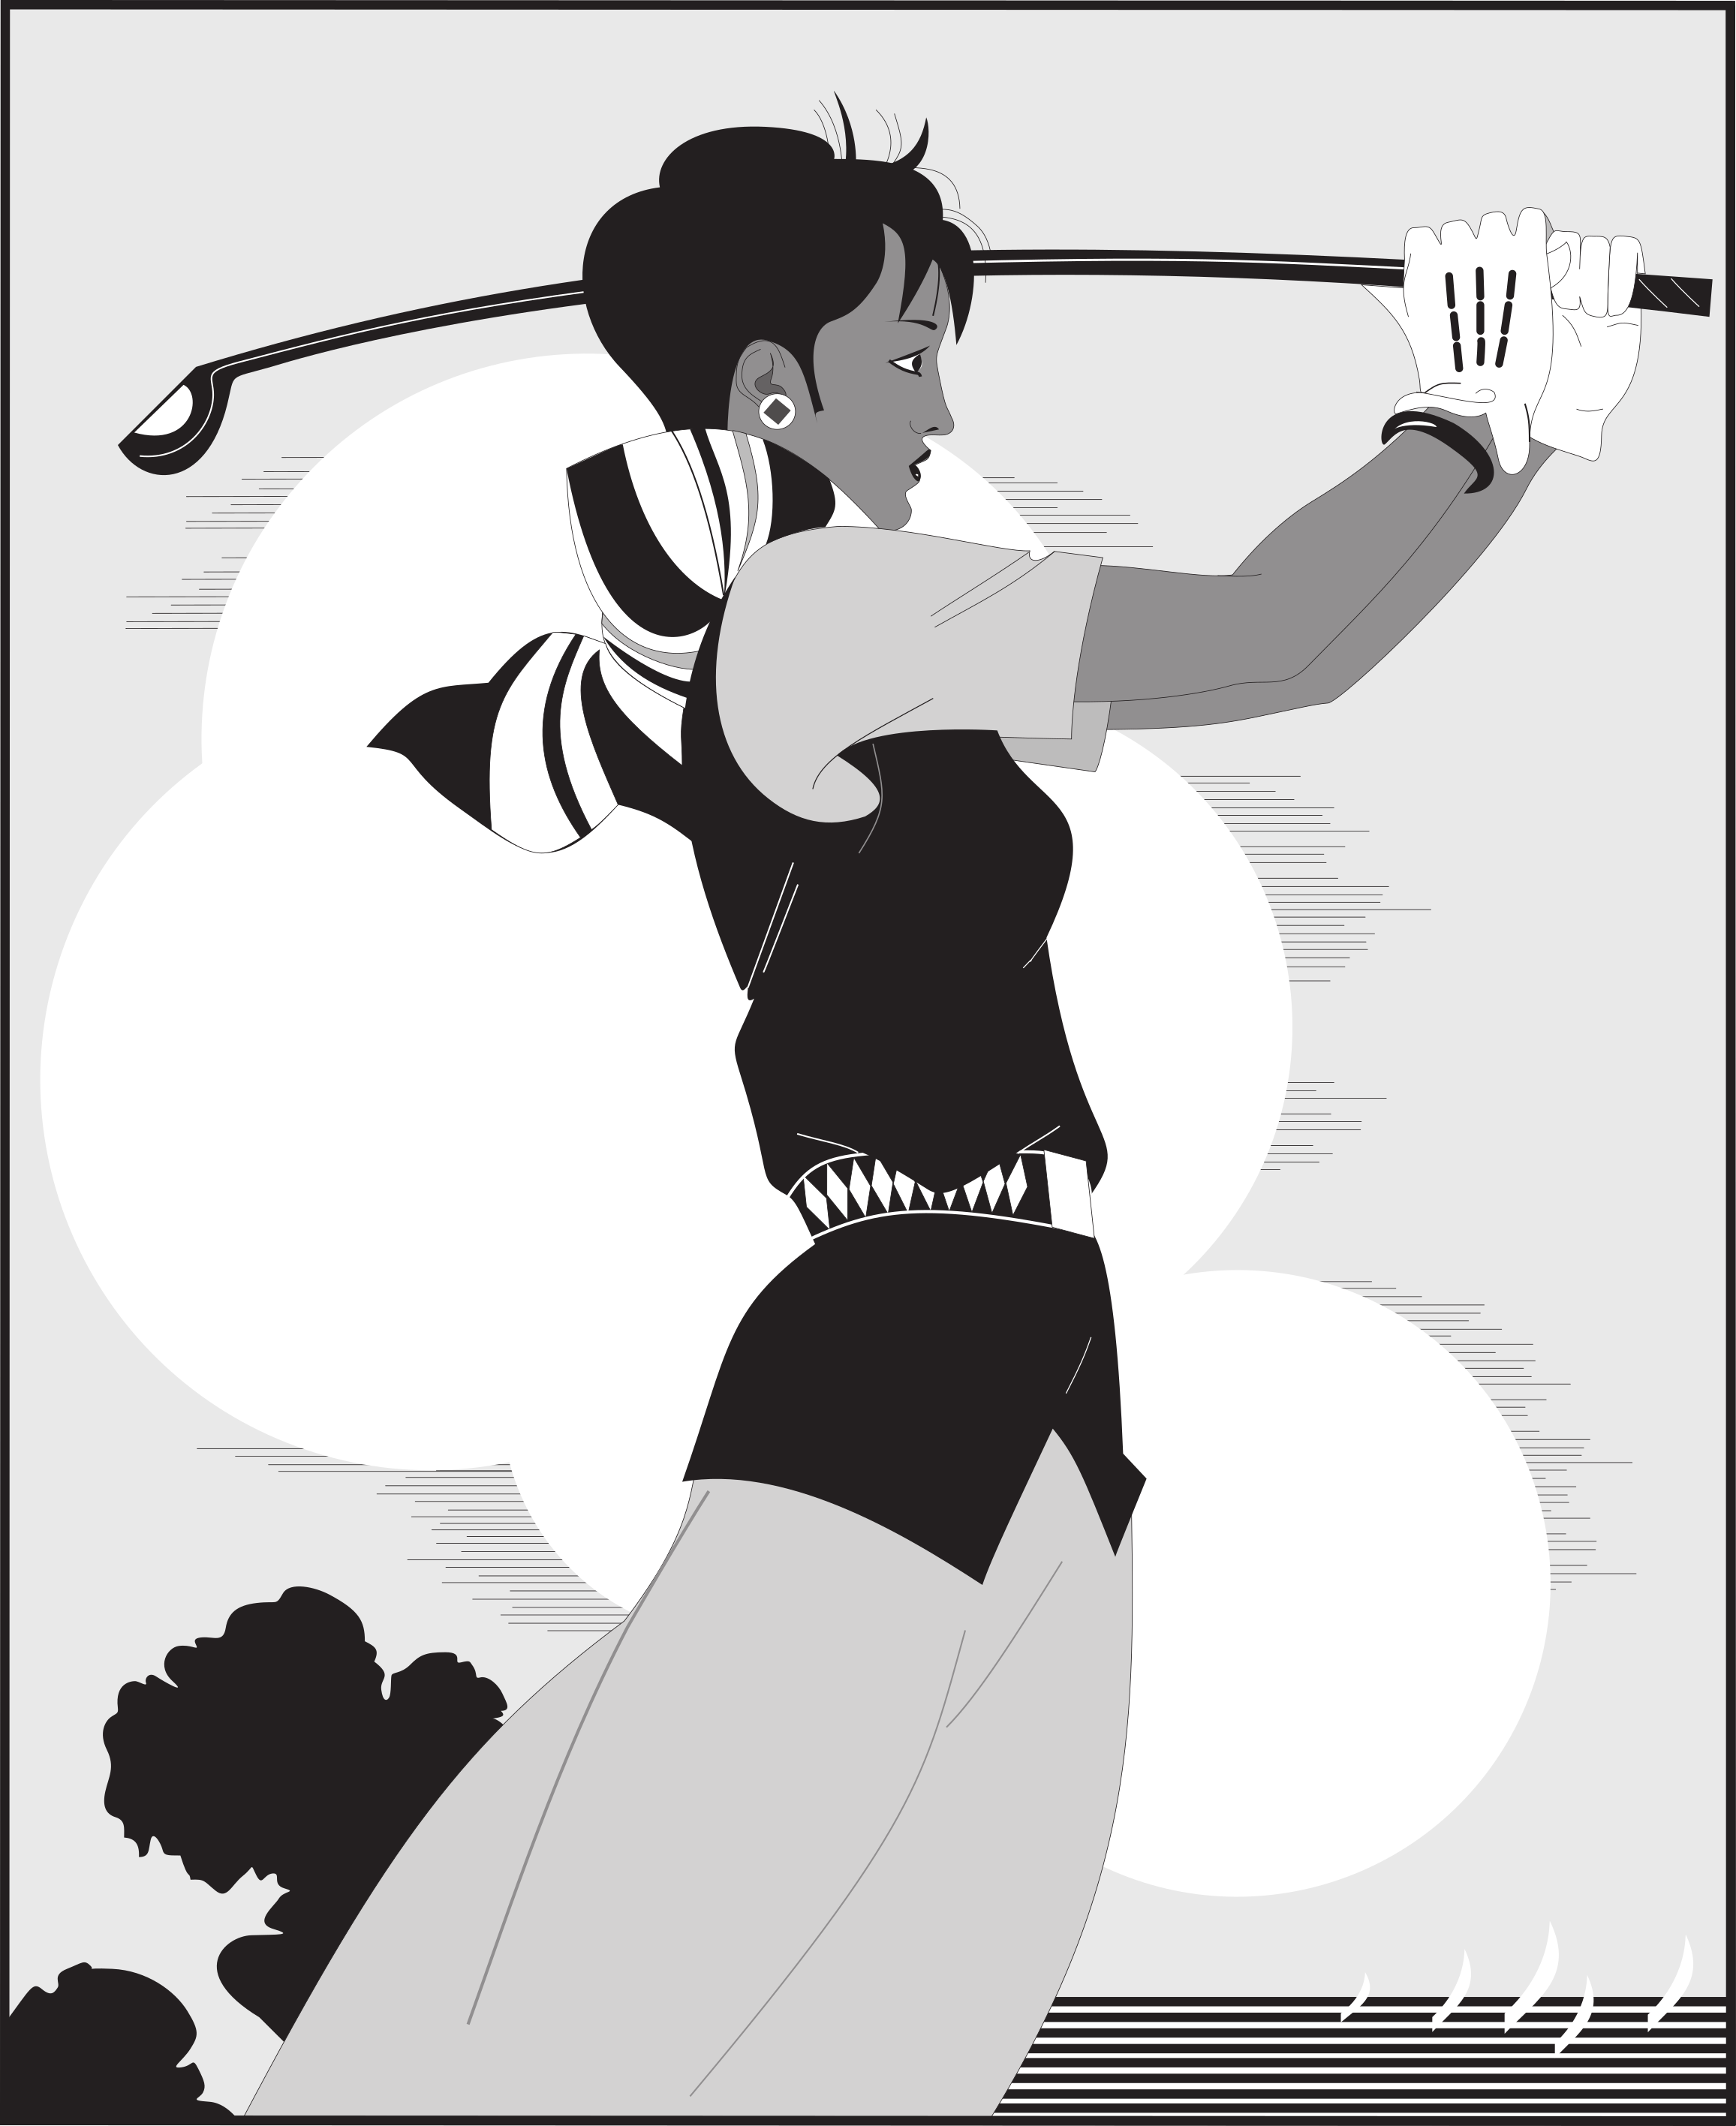
\includegraphics[width=0.2\textwidth]{golfer}}
			\fbox{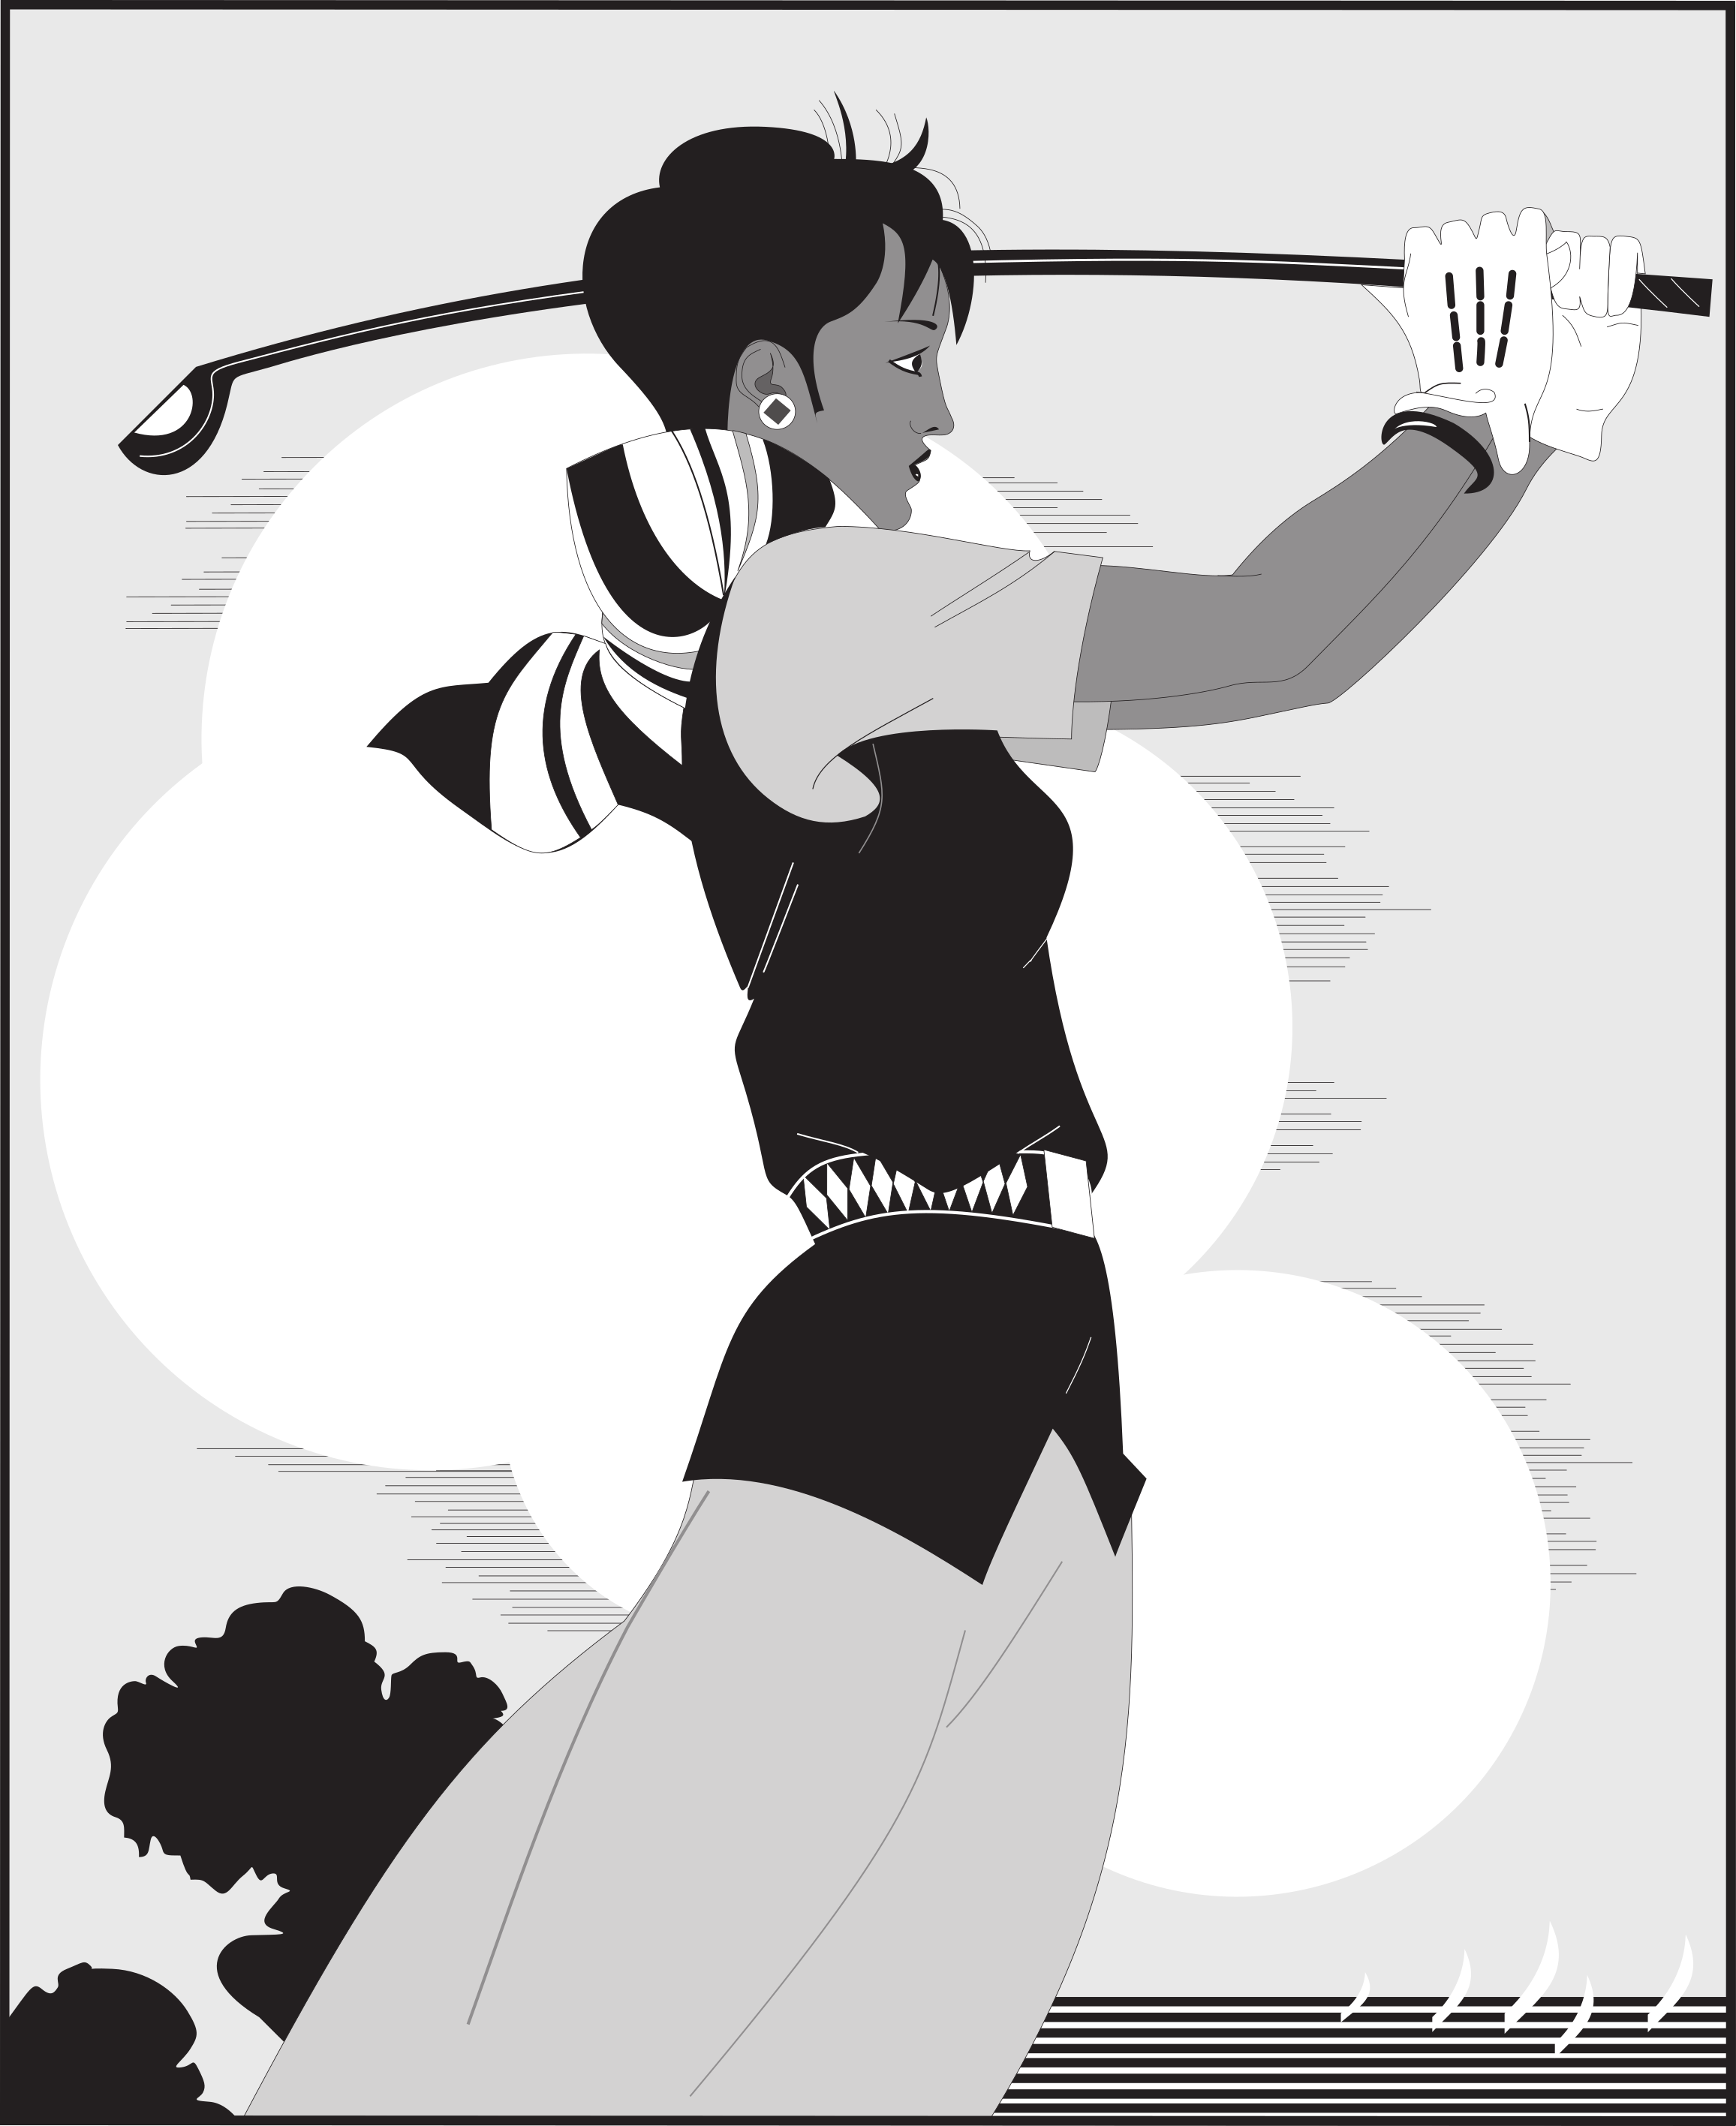
\includegraphics[width=0.2\textwidth]{golfer}}
			\fbox{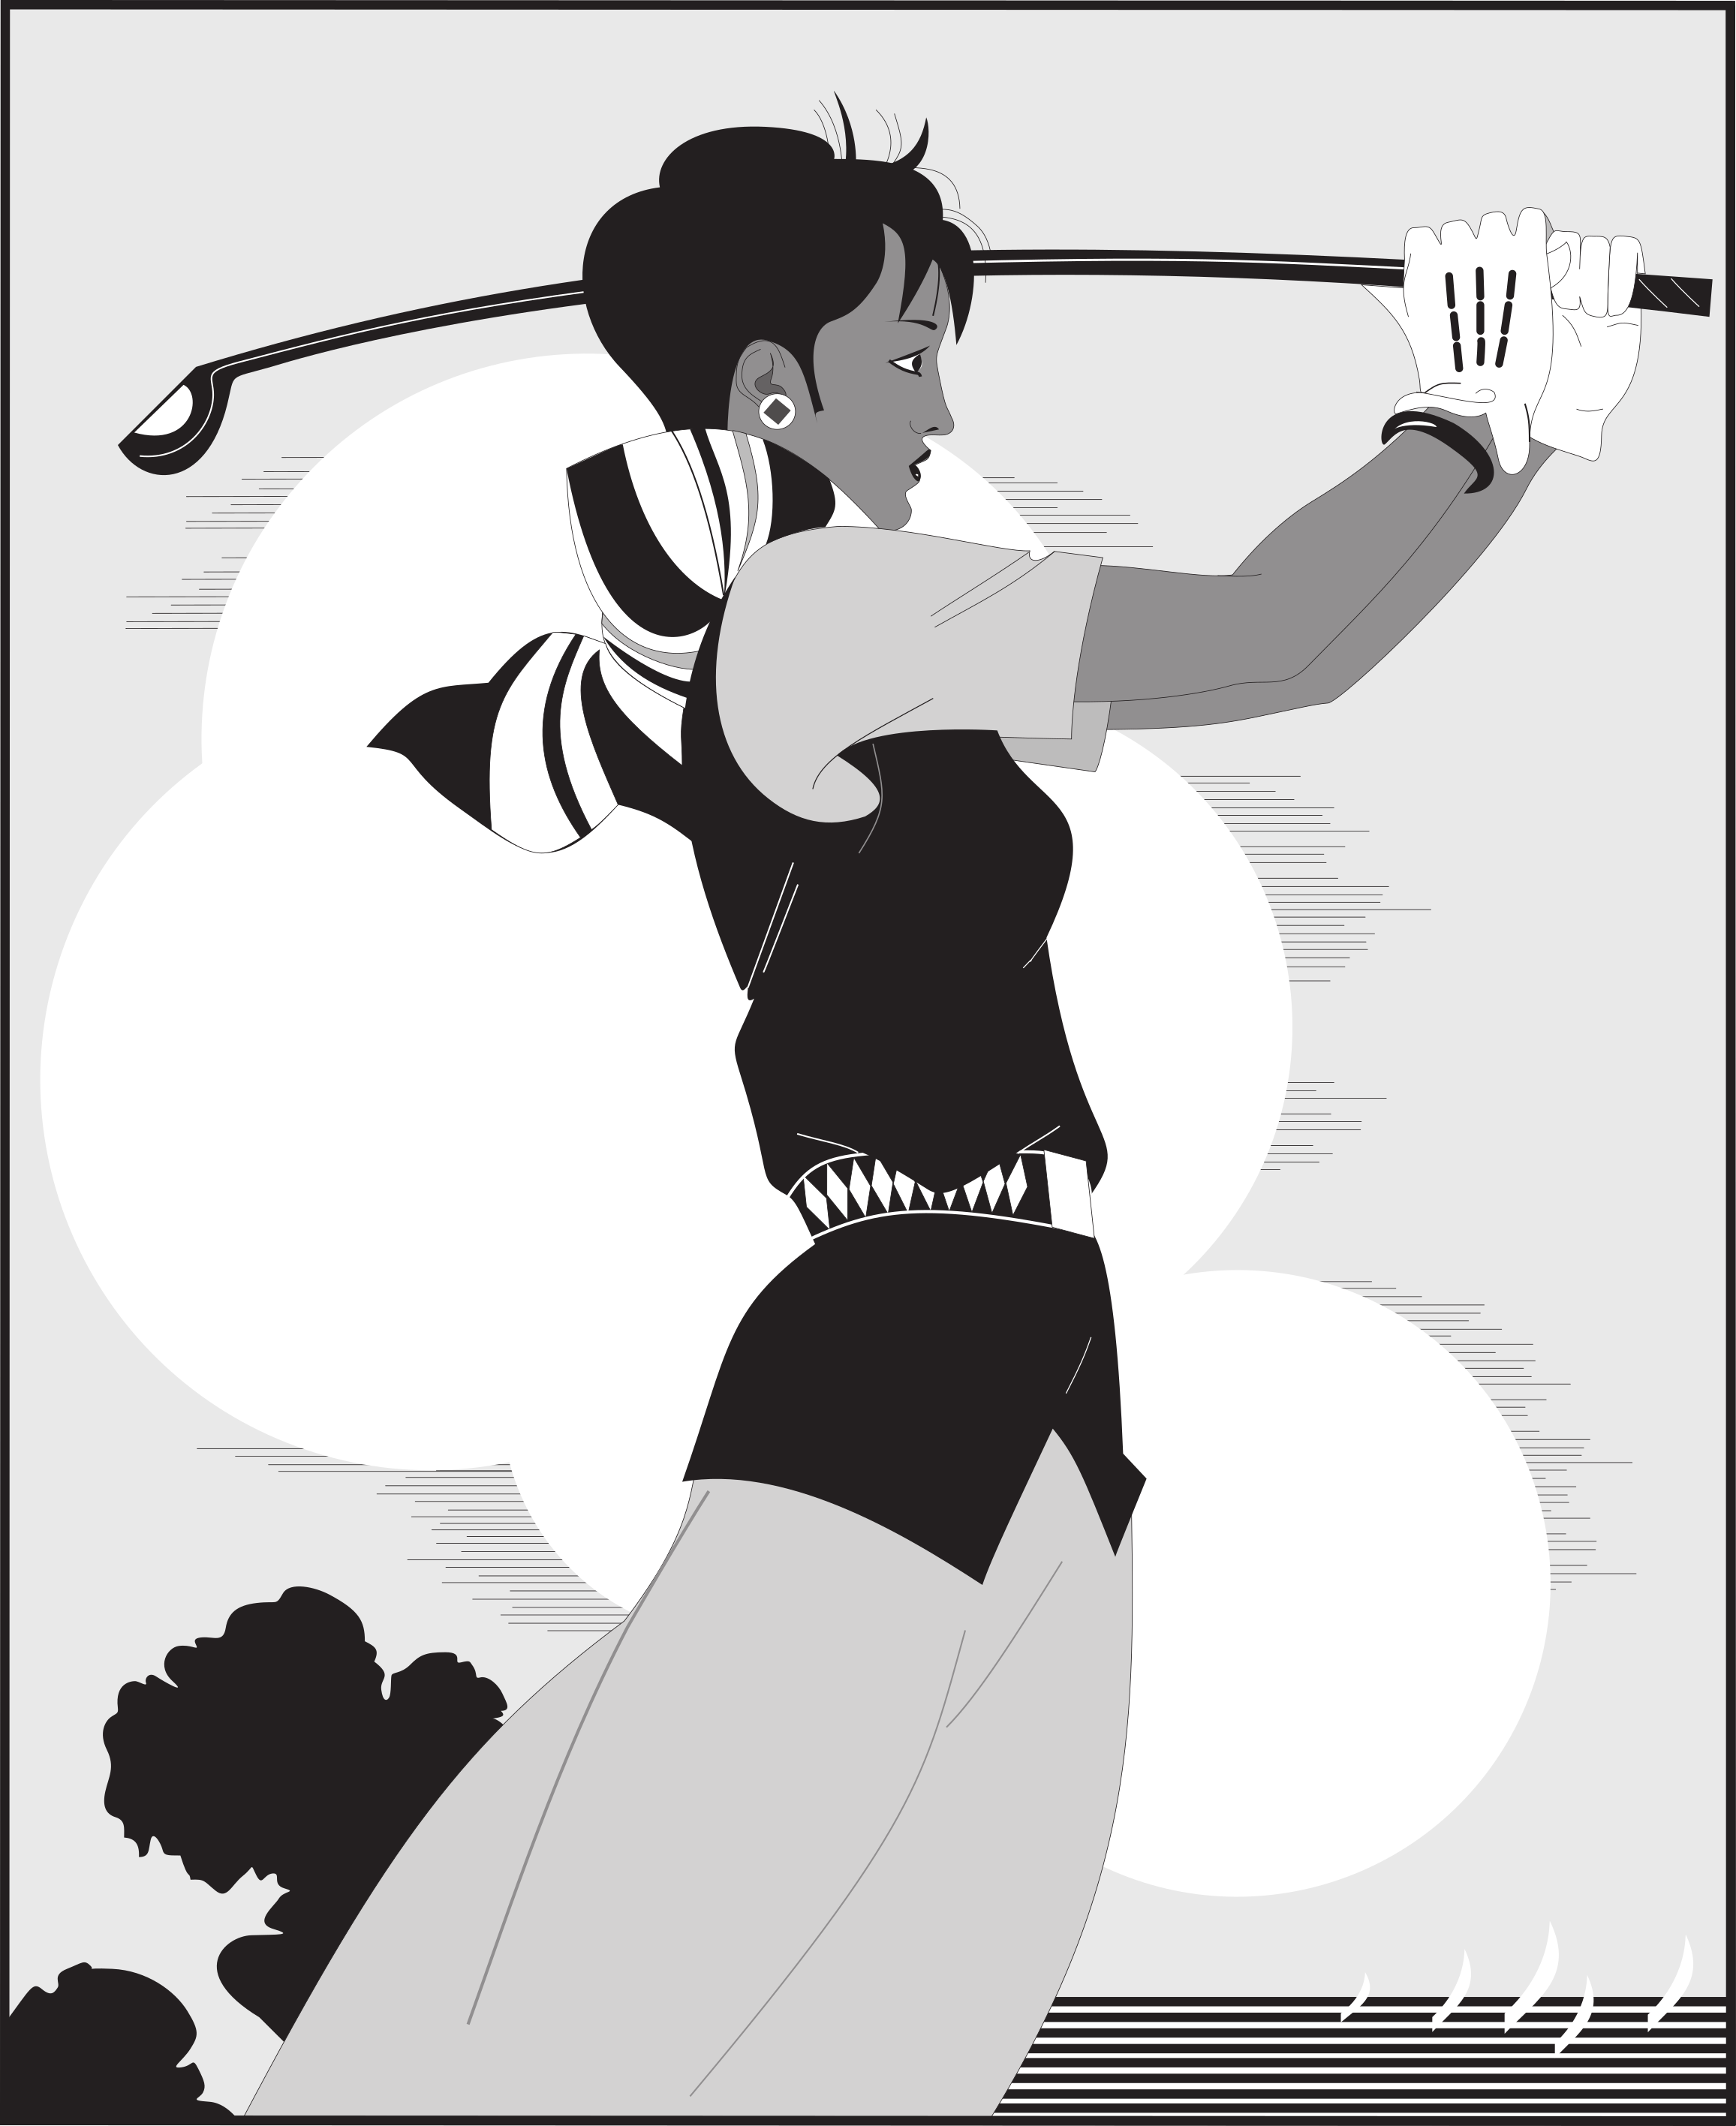
\includegraphics[width=0.2\textwidth]{golfer}}
			\fbox{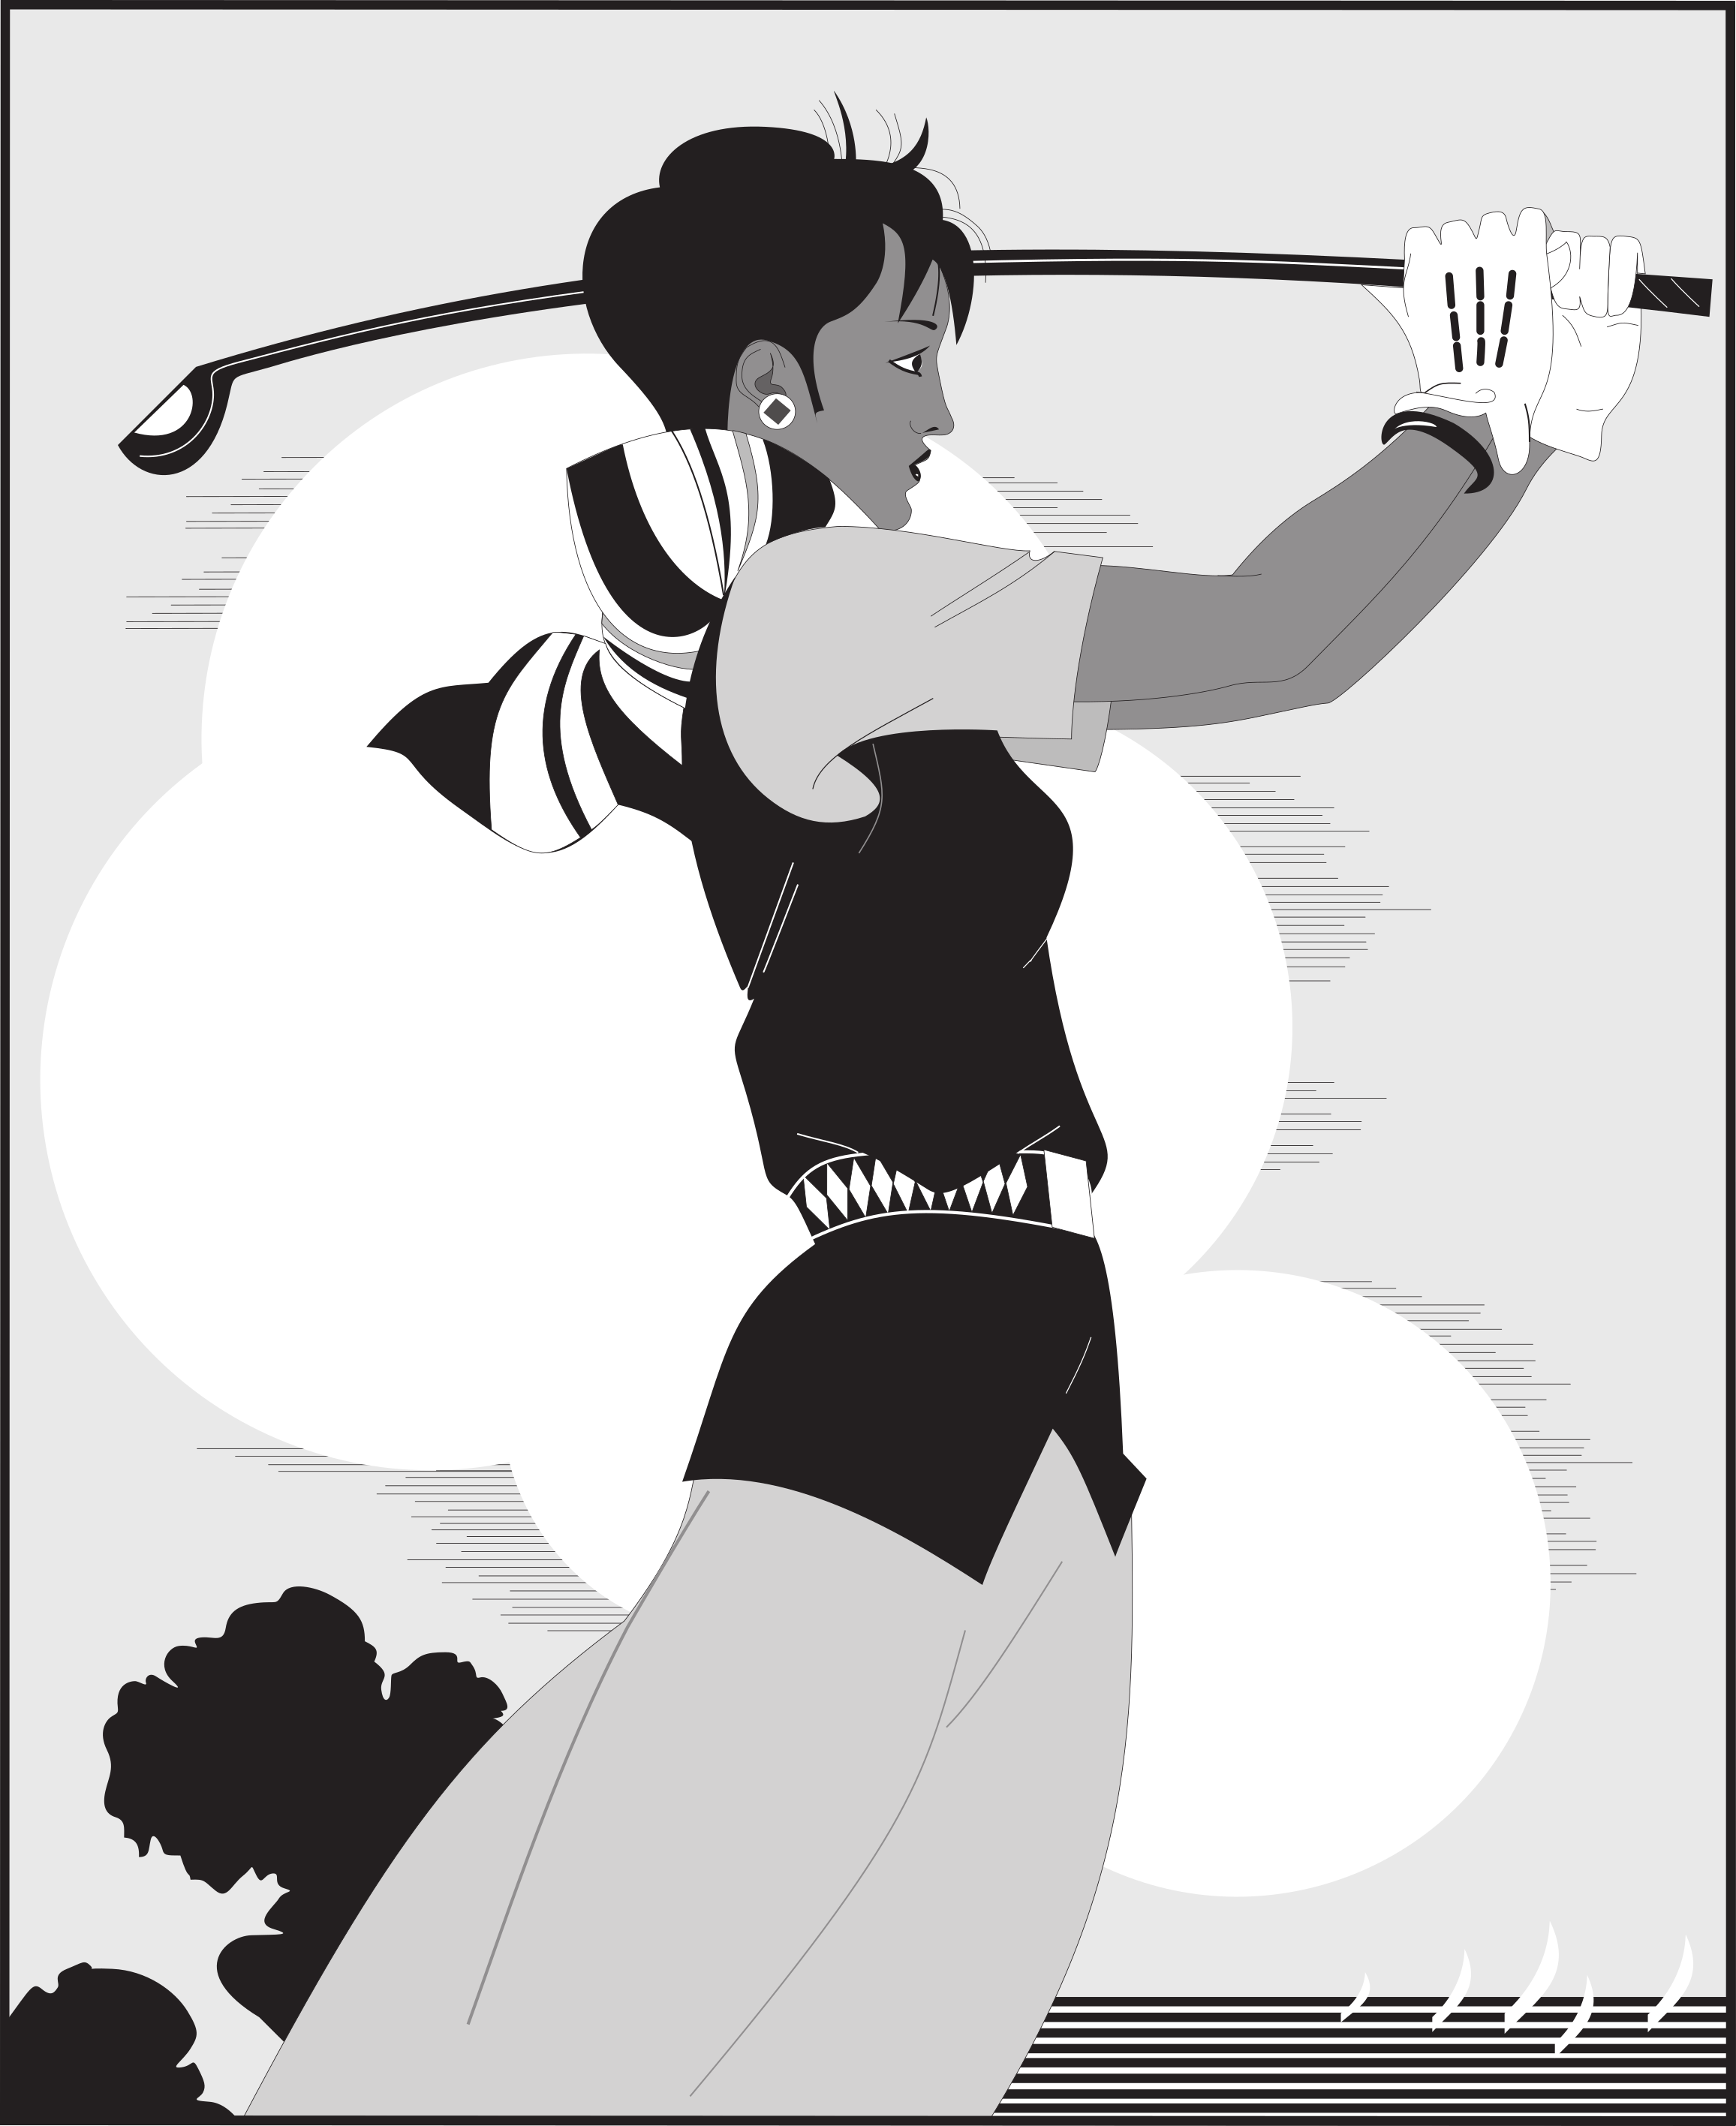
\includegraphics[width=0.2\textwidth]{golfer}}
			\fbox{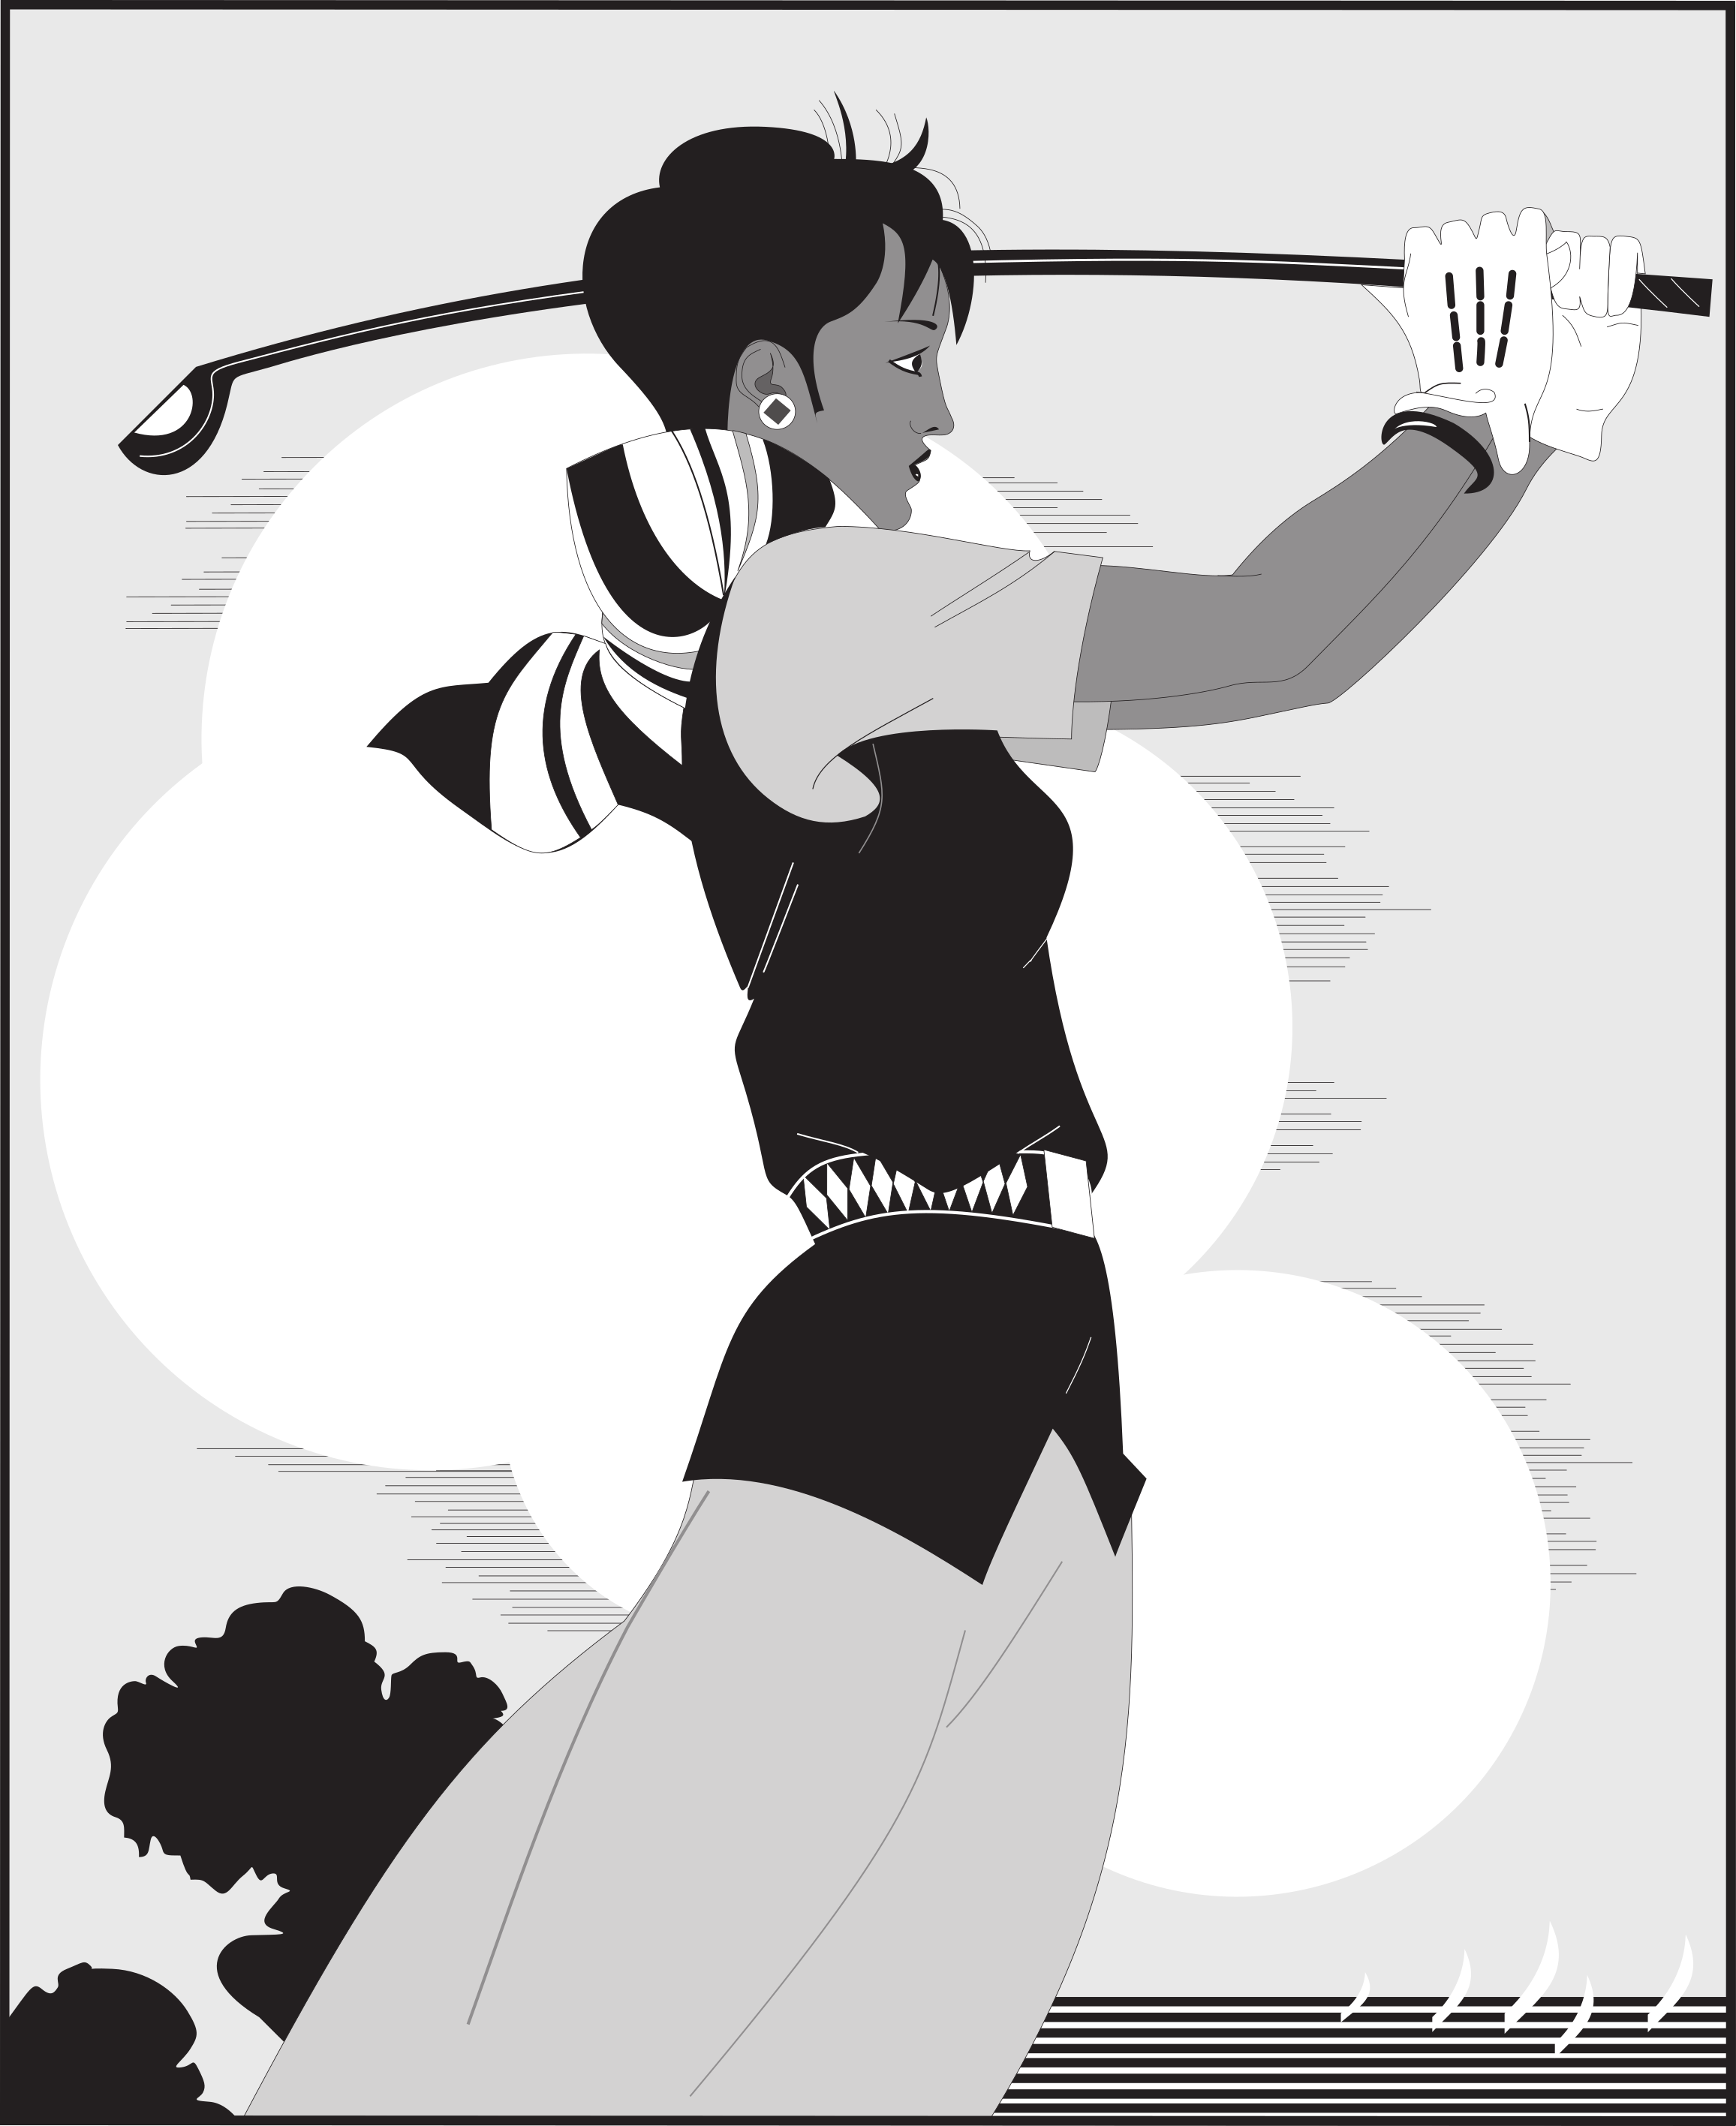
\includegraphics[width=0.2\textwidth]{golfer}}
\bicaption[golfer7]{}{打高尔夫球的人(非规范要求)}{Fig.$\!$}{The person playing golf (Not stated in the regulation)}
		\end{minipage}
	\end{sideways}
\end{figure}

\clearpage

如果不想让图片浮动到下一章节,那么在此处使用\cs{clearpage}命令。

\section{如何做出符合规范的漂亮的图}
关于作图工具在后文\ref{drawtool}中给出一些作图工具的介绍,此处不多言。
此处以R语言和Tikz为例说明如何做出符合规范的图。

\subsection{Tikz作图举例}
使用Tikz作图核心思想是把格式、主题、样式与内容分离,定义在全局中。
注意字体设置可以有两种选择,如何字少,用五号字,字多用小五。
使用Tikz作图不会出现字体问题,字体会自动与正文一致。

\begin{figure}[thb!]
  \centering
      \begin{tikzpicture}[xscale=0.8,yscale=0.3,rotate=90]
        \small
	\draw (-22,6.5) node[refcell]{参考基因组};
	\draw[refline] (-23, 5) -- (27, 5);
	\draw (-22,3.75) node[tscell]{肿瘤样本};
	\draw (-20,3.75) node[tncell]{正常细胞};
	\draw[tnline] (-21, 2.5) -- (27, 2.5);
	\draw (-20,1.25) node[ttcell]{肿瘤细胞};
	\rcell{2}{6};
	\draw[fakeevolve] (4.5, 5.25) -- (4.5, 4.8);
	\ncell{2}{4};
	\draw[evolve] (4.5, 3) .. controls (4.5,2.8) and (-3.5,2.9) ..  (-3.5, 2);
	\draw[evolve] (4.5, 3) .. controls (4.5,2.8) and (11.5,2.9) .. (11.5, 2);
	\tcellone{-6}{1.5};
	\draw (-9, 2) node[ttcell]{1};
	\draw[evolve] (-3.5, 0) .. controls (-3.5,-0.2) and (-12,-0.1) .. (-12, -1.5);
	\draw[evolve] (-3.5, 0) .. controls (-3.5,-0.2) and (1.5,-0.1) .. (1.5, -1.5);
	\tcellthree{7}{1.5};
	\draw (4, 2) node[ttcell]{2};
	\draw[evolve] (11, 0.5) .. controls (11,0.3) and (19,0.4) .. (19, -1.5);
	\tcellfive{-16}{-2};
	\draw (-19, -1.5) node[ttcell]{3};
	\tcelltwo{-1}{-2};
	\draw (-4, -1.5) node[ttcell]{4};
	\tcellfour{12}{-2};
	\draw (9, -1.5) node[ttcell]{5};
      \end{tikzpicture}
  \begin{minipage}{.9\linewidth}
      \vskip 0.2em
      \wuhao 图中,带有箭头的淡蓝色箭头表示肿瘤子种群的进化方向。一般地,从肿瘤组织中取用于进行二代测序的样本中含有一定程度的正常细胞污染,因此肿瘤的样本中含有正常细胞和肿瘤细胞。每一个子种群的基因组的模拟过程是把生殖细胞变异和体细胞变异加入到参考基因组中。
      \vspace{0.6em}
  \end{minipage}
\bicaption[tumor]{}{肿瘤组织中各个子种群的进化示意图}{Fig.$\!$}{The diagram of tumor subpopulation evolution process}
\end{figure}

\subsection{R作图}
R是一种极具有代表性的典型的作图工具,应用广泛。
与Tikz图~\ref{tumor}~不同,R作图分两种情况:(1)可以转换为Tikz码;(2)不可转换为Tikz码。
第一种情况图形简单,图形中不含有很多数据点,使用R语言中的Tikz包即可。
第二种情况是图形复杂,含有海量数据点,这时候不要转成Tikz矢量图,这会使得论文体积巨大。
推荐使用pdf或png非矢量图形。
使用非矢量图形时要注意选择好字号(五号或小五),和字体(宋体、新罗马)然后选择生成图形大小,注意此时在正文中使用\cs{includegraphics}命令导入时,不要像导入矢量图那样控制图形大小,使用图形的原本的
宽度和高度,这样就确保了非矢量图形中的文字与正文一致了。

为了控制\hithesis\ 的大小,此处不给出具体举例,

\section{表格}

表应有自明性。表格不加左、右边线。表的编排建议采用国际通行的三线表。表中文字用宋
体~5~号字。每个表格均应有表题(由表序和表名组成)。表序一般按章编排,如第~1~章第
一个插表的序号为“表~1-1”等。表序与表名之间空一格,表名中不允许使用标点符号,表名
后不加标点。表题置于表上,硕士学位论文只用中文,博士学位论文用中、英文两种文字居
中排写,中文在上,要求中文用宋体~5~号字,英文用新罗马字体~5~号字。表头设计应简单
明了,尽量不用斜线。表头中可采用化学符号或物理量符号。


\subsection{普通表格的绘制方法}[Methods of drawing normal tables]

表格应具有三线表格式,因此需要调用~booktabs~宏包,其标准格式如表~\ref{table1}~所示。
\begin{table}[htbp]
\bicaption[table1]{}{符合研究生院绘图规范的表格}{Table$\!$}{Table in agreement of the standard from graduate school}
\vspace{0.5em}\centering\wuhao
\begin{tabular}{ccccc}
\toprule[1.5pt]
$D$(in) & $P_u$(lbs) & $u_u$(in) & $\beta$ & $G_f$(psi.in)\\
\midrule[1pt]
 5 & 269.8 & 0.000674 & 1.79 & 0.04089\\
10 & 421.0 & 0.001035 & 3.59 & 0.04089\\
20 & 640.2 & 0.001565 & 7.18 & 0.04089\\
\bottomrule[1.5pt]
\end{tabular}
\end{table}
全表如用同一单位,则将单位符号移至表头右上角,加圆括号。表中数据应准确无误,书写
清楚。数字空缺的格内加横线“-”(占~2~个数字宽度)。表内文字或数字上、下或左、右
相同时,采用通栏处理方式,不允许用“〃”、“同上”之类的写法。表内文字说明,起行空一
格、转行顶格、句末不加标点。如某个表需要转页接排,在随后的各页上应重复表的编号。
编号后加“(续表)”,表题可省略。续表应重复表头。

\subsection{长表格的绘制方法}[Methods of drawing long tables]

长表格是当表格在当前页排不下而需要转页接排的情况下所采用的一种表格环境。若长表格
仍按照普通表格的绘制方法来获得,其所使用的\verb|table|浮动环境无法实现表格的换页
接排功能,表格下方过长部分会排在表格第1页的页脚以下。为了能够实现长表格的转页接
排功能,需要调用~longtable~宏包,由于长表格是跨页的文本内容,因此只需要单独的
\verb|longtable|环境,所绘制的长表格的格式如表~\ref{table2}~所示。

注意,长表格双语标题的格式。

\vspace{-1.5bp}
\ltfontsize{\wuhao[1.667]}
\wuhao[1.667]\begin{longtable}{ccc}%
\longbionenumcaption{}{{\wuhao 中国省级行政单位一览
}\label{table3}}{Table$\!$}{}{{\wuhao Overview of the provincial administrative
unit of China}}{-0.5em}{3.15bp}\\
%\caption{\wuhao 中国省级行政单位一览}\\
\toprule[1.5pt] 名称 & 简称 & 省会或首府  \\ \midrule[1pt]
\endfirsthead
\multicolumn{3}{r}{表~\thetable(续表)}\vspace{0.5em}\\
\toprule[1.5pt] 名称 & 简称 & 省会或首府  \\ \midrule[1pt]
\endhead
\bottomrule[1.5pt]
\endfoot
北京市 & 京 & 北京\\
天津市 & 津 & 天津\\
河北省 & 冀 & 石家庄市\\
山西省 & 晋 & 太原市\\
内蒙古自治区 & 蒙 & 呼和浩特市\\
辽宁省 & 辽 & 沈阳市\\
吉林省 & 吉 & 长春市\\
黑龙江省 & 黑 & 哈尔滨市\\
上海市 & 沪/申 & 上海\\
江苏省 & 苏 & 南京市\\
浙江省 & 浙 & 杭州市\\
安徽省 & 皖 & 合肥市\\
福建省 & 闽 & 福州市\\
江西省 & 赣 & 南昌市\\
山东省 & 鲁 & 济南市\\
河南省 & 豫 & 郑州市\\
湖北省 & 鄂 & 武汉市\\
湖南省 & 湘 & 长沙市\\
广东省 & 粤 & 广州市\\
广西壮族自治区 & 桂 & 南宁市\\
海南省 & 琼 & 海口市\\
重庆市 & 渝 & 重庆\\
四川省 & 川/蜀 & 成都市\\
贵州省 & 黔/贵 & 贵阳市\\
云南省 & 云/滇 & 昆明市\\
西藏自治区 & 藏 & 拉萨市\\
陕西省 & 陕/秦 & 西安市\\
甘肃省 & 甘/陇 & 兰州市\\
青海省 & 青 & 西宁市\\
宁夏回族自治区 & 宁 & 银川市\\
新疆维吾尔自治区 & 新 & 乌鲁木齐市\\
香港特别行政区 & 港 & 香港\\
澳门特别行政区 & 澳 & 澳门\\
台湾省 & 台 & 台北市\\
\end{longtable}\normalsize
\vspace{-1em}

此长表格~\ref{table2}~第~2~页的标题“编号(续表)”和表头是通过代码自动添加上去的,无需人工添加,若表格在页面中的竖直位置发生了变化,长表格在第~2~页
及之后各页的标题和表头位置能够始终处于各页的最顶部,也无需人工调整,\LaTeX~系统的这一优点是~word~等软件所无法比拟的。

\subsection{列宽可调表格的绘制方法}[Methods of drawing tables with adjustable-width columns]
论文中能用到列宽可调表格的情况共有两种,一种是当插入的表格某一单元格内容过长以至
于一行放不下的情况,另一种是当对公式中首次出现的物理量符号进行注释的情况,这两种
情况都需要调用~tabularx~宏包。下面将分别对这两种情况下可调表格的绘制方法进行阐述
。
\subsubsection{表格内某单元格内容过长的情况}[The condition when the contents in
some cells of tables are too long]
首先给出这种情况下的一个例子如表~\ref{table3}~所示。
\begin{table}[htbp]
  \centering
\bicaption[table4]{}{最小的三个正整数的英文表示法}{Table$\!$}{The English construction of the smallest three positive integral numbers}\vspace{0.5em}\wuhao
\begin{tabularx}{0.7\textwidth}{llX}
\toprule[1.5pt]
Value & Name & Alternate names, and names for sets of the given size\\\midrule[1pt]
1 & One & ace, single, singleton, unary, unit, unity\\
2 & Two & binary, brace, couple, couplet, distich, deuce, double, doubleton, duad, duality, duet, duo, dyad, pair, snake eyes, span, twain, twosome, yoke\\
3 & Three & deuce-ace, leash, set, tercet, ternary, ternion, terzetto, threesome, tierce, trey, triad, trine, trinity, trio, triplet, troika, hat-trick\\\bottomrule[1.5pt]
\end{tabularx}
\end{table}
tabularx环境共有两个必选参数:第1个参数用来确定表格的总宽度,第2个参数用来确定每
列格式,其中标为X的项表示该列的宽度可调,其宽度值由表格总宽度确定。标为X的列一般
选为单元格内容过长而无法置于一行的列,这样使得该列内容能够根据表格总宽度自动分行
。若列格式中存在不止一个X项,则这些标为X的列的列宽相同,因此,一般不将内容较短的
列设为X。标为X的列均为左对齐,因此其余列一般选为l(左对齐),这样可使得表格美观
,但也可以选为c或r。

\subsubsection{对物理量符号进行注释的情况}[The condition when physical symbols
need to be annotated]

为使得对公式中物理量符号注释的转行与破折号“———”后第一个字对齐,此处最好采用表格
环境。此表格无任何线条,左对齐,且在破折号处对齐,一共有“式中”二字、物理量符号和
注释三列,表格的总宽度可选为文本宽度,因此应该采用\verb|tabularx|环境。由
\verb|tabularx|环境生成的对公式中物理量符号进行注释的公式如式(\ref{eq:1})所示。
\begin{equation}\label{eq:1}
\ddot{\boldsymbol{\rho}}-\frac{\mu}{R_{t}^{3}}\left(3\mathbf{R_{t}}\frac{\mathbf{R_{t}\rho}}{R_{t}^{2}}-\boldsymbol{\rho}\right)=\mathbf{a}
\end{equation}
\begin{tabularx}{\textwidth}{@{}l@{\quad}r@{———}X@{}}
式中& $\boldsymbol{\rho}$ &追踪飞行器与目标飞行器之间的相对位置矢量;\\
&  $\boldsymbol{\ddot{\rho}}$&追踪飞行器与目标飞行器之间的相对加速度;\\
&  $\mathbf{a}$   &推力所产生的加速度;\\
&  $\mathbf{R_t}$ & 目标飞行器在惯性坐标系中的位置矢量;\\
&  $\omega_{t}$ & 目标飞行器的轨道角速度;\\
&  $\mathbf{g}$ & 重力加速度,$=\frac{\mu}{R_{t}^{3}}\left(
3\mathbf{R_{t}}\frac{\mathbf{R_{t}\rho}}{R_{t}^{2}}-\boldsymbol{\rho}\right)=\omega_{t}^{2}\frac{R_{t}}{p}\left(
3\mathbf{R_{t}}\frac{\mathbf{R_{t}\rho}}{R_{t}^{2}}-\boldsymbol{\rho}\right)$,这里~$p$~是目标飞行器的轨道半通径。
\end{tabularx}\vspace{3.15bp}
由此方法生成的注释内容应紧邻待注释公式并置于其下方,因此不能将代码放入
\verb|table|浮动环境中。但此方法不能实现自动转页接排,可能会在当前页剩余空间不够
时,全部移动到下一页而导致当前页出现很大空白。因此在需要转页处理时,还请您手动将
需要转页的代码放入一个新的\verb|tabularx|环境中,将原来的一个\verb|tabularx|环境
拆分为两个\verb|tabularx|环境。

\subsubsection{排版横版表格的举例}[An example of landscape table]

\begin{table}[p]
\centering
\begin{sideways}
\begin{minipage}{\textheight}
\bicaption[table2]{}{不在规范中规定的横版表格}{Table$\!$}{A table style which is not stated in the regulation}
\vspace{0.5em}\centering\wuhao
\begin{tabular}{ccccc}
\toprule[1.5pt]
$D$(in) & $P_u$(lbs) & $u_u$(in) & $\beta$ & $G_f$(psi.in)\\
\midrule[1pt]
 5 & 269.8 & 0.000674 & 1.79 & 0.04089\\
10 & 421.0 & 0.001035 & 3.59 & 0.04089\\
20 & 640.2 & 0.001565 & 7.18 & 0.04089\\
\bottomrule[1.5pt]
\end{tabular}
\end{minipage}
\end{sideways}
\end{table}


\section{公式}
与正常\LaTeX\ 使用方法一致,此处略。关于公式中符号样式的定义在`hithesis.sty'有示
例。

\section{其他杂项}[Miscellaneous]

\subsection{右翻页}[Open right]

对于双面打印的论文,强制使每章的标题页出现右手边为右翻页。
规范中没有明确规定是否是右翻页打印。
模板给出了右翻页选项。
为了应对用户的个人喜好,在希望设置成右翻页的位置之前添加\cs{cleardoublepage}命令即可。

\subsection{算法}[Algorithms]
我工算法有以下几大特点。

(1)算法不在规范中要求。

(2)算法常常被使用(至少计算机学院)。

(3)格式乱,甚至出现了每个实验室的格式要求都不一样。

此处不给出示例,因为没法给,在
\href{https://github.com/dustincys/PlutoThesis}{https://github.com/dustincys/PlutoThesis}
的readme文件中有不同实验室算法要求说明。

\subsection{脚注}[Footnotes]
不在再规范\footnote{规范是指\PGR\ 和\UGR}中要求,模板默认使用清华大学的格式。

\subsection{源码}[Source code]
也不在再规范中要求。如果有需要最好使用minted包,但在编译的时候需要添加“
-shell-escape”选项且安装pygmentize软件,这些不在模板中默认载入,如果需要自行载入
。
\subsection{思源宋体}[Siyuan font]
如果要使用思源字体,需要思源字体的定义文件,此文件请到模板的开发版网址github:
\href{https://github.com/dustincys/hithesis}{https://github.com/dustincys/hithesis}
或者oschia:
\href{https://git.oschina.net/dustincys/hithesis}{https://git.oschina.net/dustincys/hithesis}
处下载。

\subsection{专业绘图工具}[Processional drawing tool]
\label{drawtool}
推荐使用tikz包,使用tikz源码绘图的好处是,图片中的字体与正文中的字体一致。具体如
何使用tikz绘图不属于模板范畴。
tikz适合用来画不需要大量实验数据支撑示意图。但R语言等专业绘图工具具有画出各种、
专业、复杂的数据图。R语言中有tikz包,能自动生成tikz码,这样tikz几乎无所不能。
对于排版有极致追求的小伙伴,可以参考
\href{http://www.texample.net/tikz/resources/}{http://www.texample.net/tikz/resources/}
中所列工具,几乎所有作图软件所作的图形都可转成tikz,然后可以自由的在tikz中修改
图中内容,定义字体等等。实现前文窝工规范中要求的图中字体的一致性的终极目标。


\subsection{术语词汇管理}[Manage glossaries]
推荐使用glossaries包管理术语、缩略语,可以自动生成首次全写,非首次缩写。

\subsection{\TeX\ 源码编辑器}[\TeX editor]
推荐:(1)付费软件Winedt;(2)免费软件kile;(3)vim或emaces或sublime等神级编
译器(需要配置)。

\subsection{\LaTeX\ 排版重要原则}[\LaTeX\ typesetting rules]
格式和内容分离是\LaTeX\ 最大优势,所有多次出现的内容、样式等等都可以定义为简单命
令、环境。这样的好处是方便修改、管理。例如,如果想要把所有的表示向量的符号由粗体
\cs{mathbf}变换到花体\cs{mathcal},只需修改该格式的命令的定义部分,不需要像MS
word那样处处修改。总而言之,使用自定义命令和环境才是正确的使用\LaTeX\ 的方式。




% Local Variables:
% TeX-master: "../main"
% TeX-engine: xetex
% End:


\backmatter
% !Mode:: "TeX:UTF-8" 
\begin{conclusions}

学位论文的结论作为论文正文的最后一章单独排写,但不加章标题序号。

结论应是作者在学位论文研究过程中所取得的创新性成果的概要总结,不能与摘要混为一谈。博士学位论文结论应包括论文的主要结果、创新点、展望三部分,在结论中应概括论文的核心观点,明确、客观地指出本研究内容的创新性成果(含新见解、新观点、方法创新、技术创新、理论创新),并指出今后进一步在本研究方向进行研究工作的展望与设想。对所取得的创新性成果应注意从定性和定量两方面给出科学、准确的评价,分(1)、(2)、(3)…条列出,宜用“提出了”、“建立了”等词叙述。

\end{conclusions}
   % 结论
\bibliographystyle{hithesis} %如果没有参考文献时候
\bibliography{reference}
%%%%%%%%%%%%%%%%%%%%%%%%%%%%%%%%%%%%%%%%%%%%%%%%%%%%%%%%%%%%%%%%%%%%%%%%%%%%%%%% 
%-- 注意:以下本硕博、博后书序不一致 --%
%%%%%%%%%%%%%%%%%%%%%%%%%%%%%%%%%%%%%%%%%%%%%%%%%%%%%%%%%%%%%%%%%%%%%%%%%%%%%%%% 
% 硕博书序
%%%%%%%%%%%%%%%%%%%%%%%%%%%%%%%%%%%%%%%%%%%%%%%%%%%%%%%%%%%%%%%%%%%%%%%%%%%%%%%% 
%\begin{appendix}%附录
%% -*-coding: utf-8 -*-
%%%%%%%%%%%%%%%%%%%%%%%%%%%%%%%%%%%%%%%%%%%%%%%%%%%%%%%%%
\chapter{带章节的附录}[Full Appendix]%
完整的附录内容,包含章节,公式,图表等

%%%%%%%%%%%%%%%%%%%%%%%%%%%%%%%%%%%%%%%%%%%%%%%%%%%%%%%%%
\section{附录节的内容}[Section in Appendix]
这是附录的节的内容

附录中图的示例:
\begin{figure}[htbp]
\centering
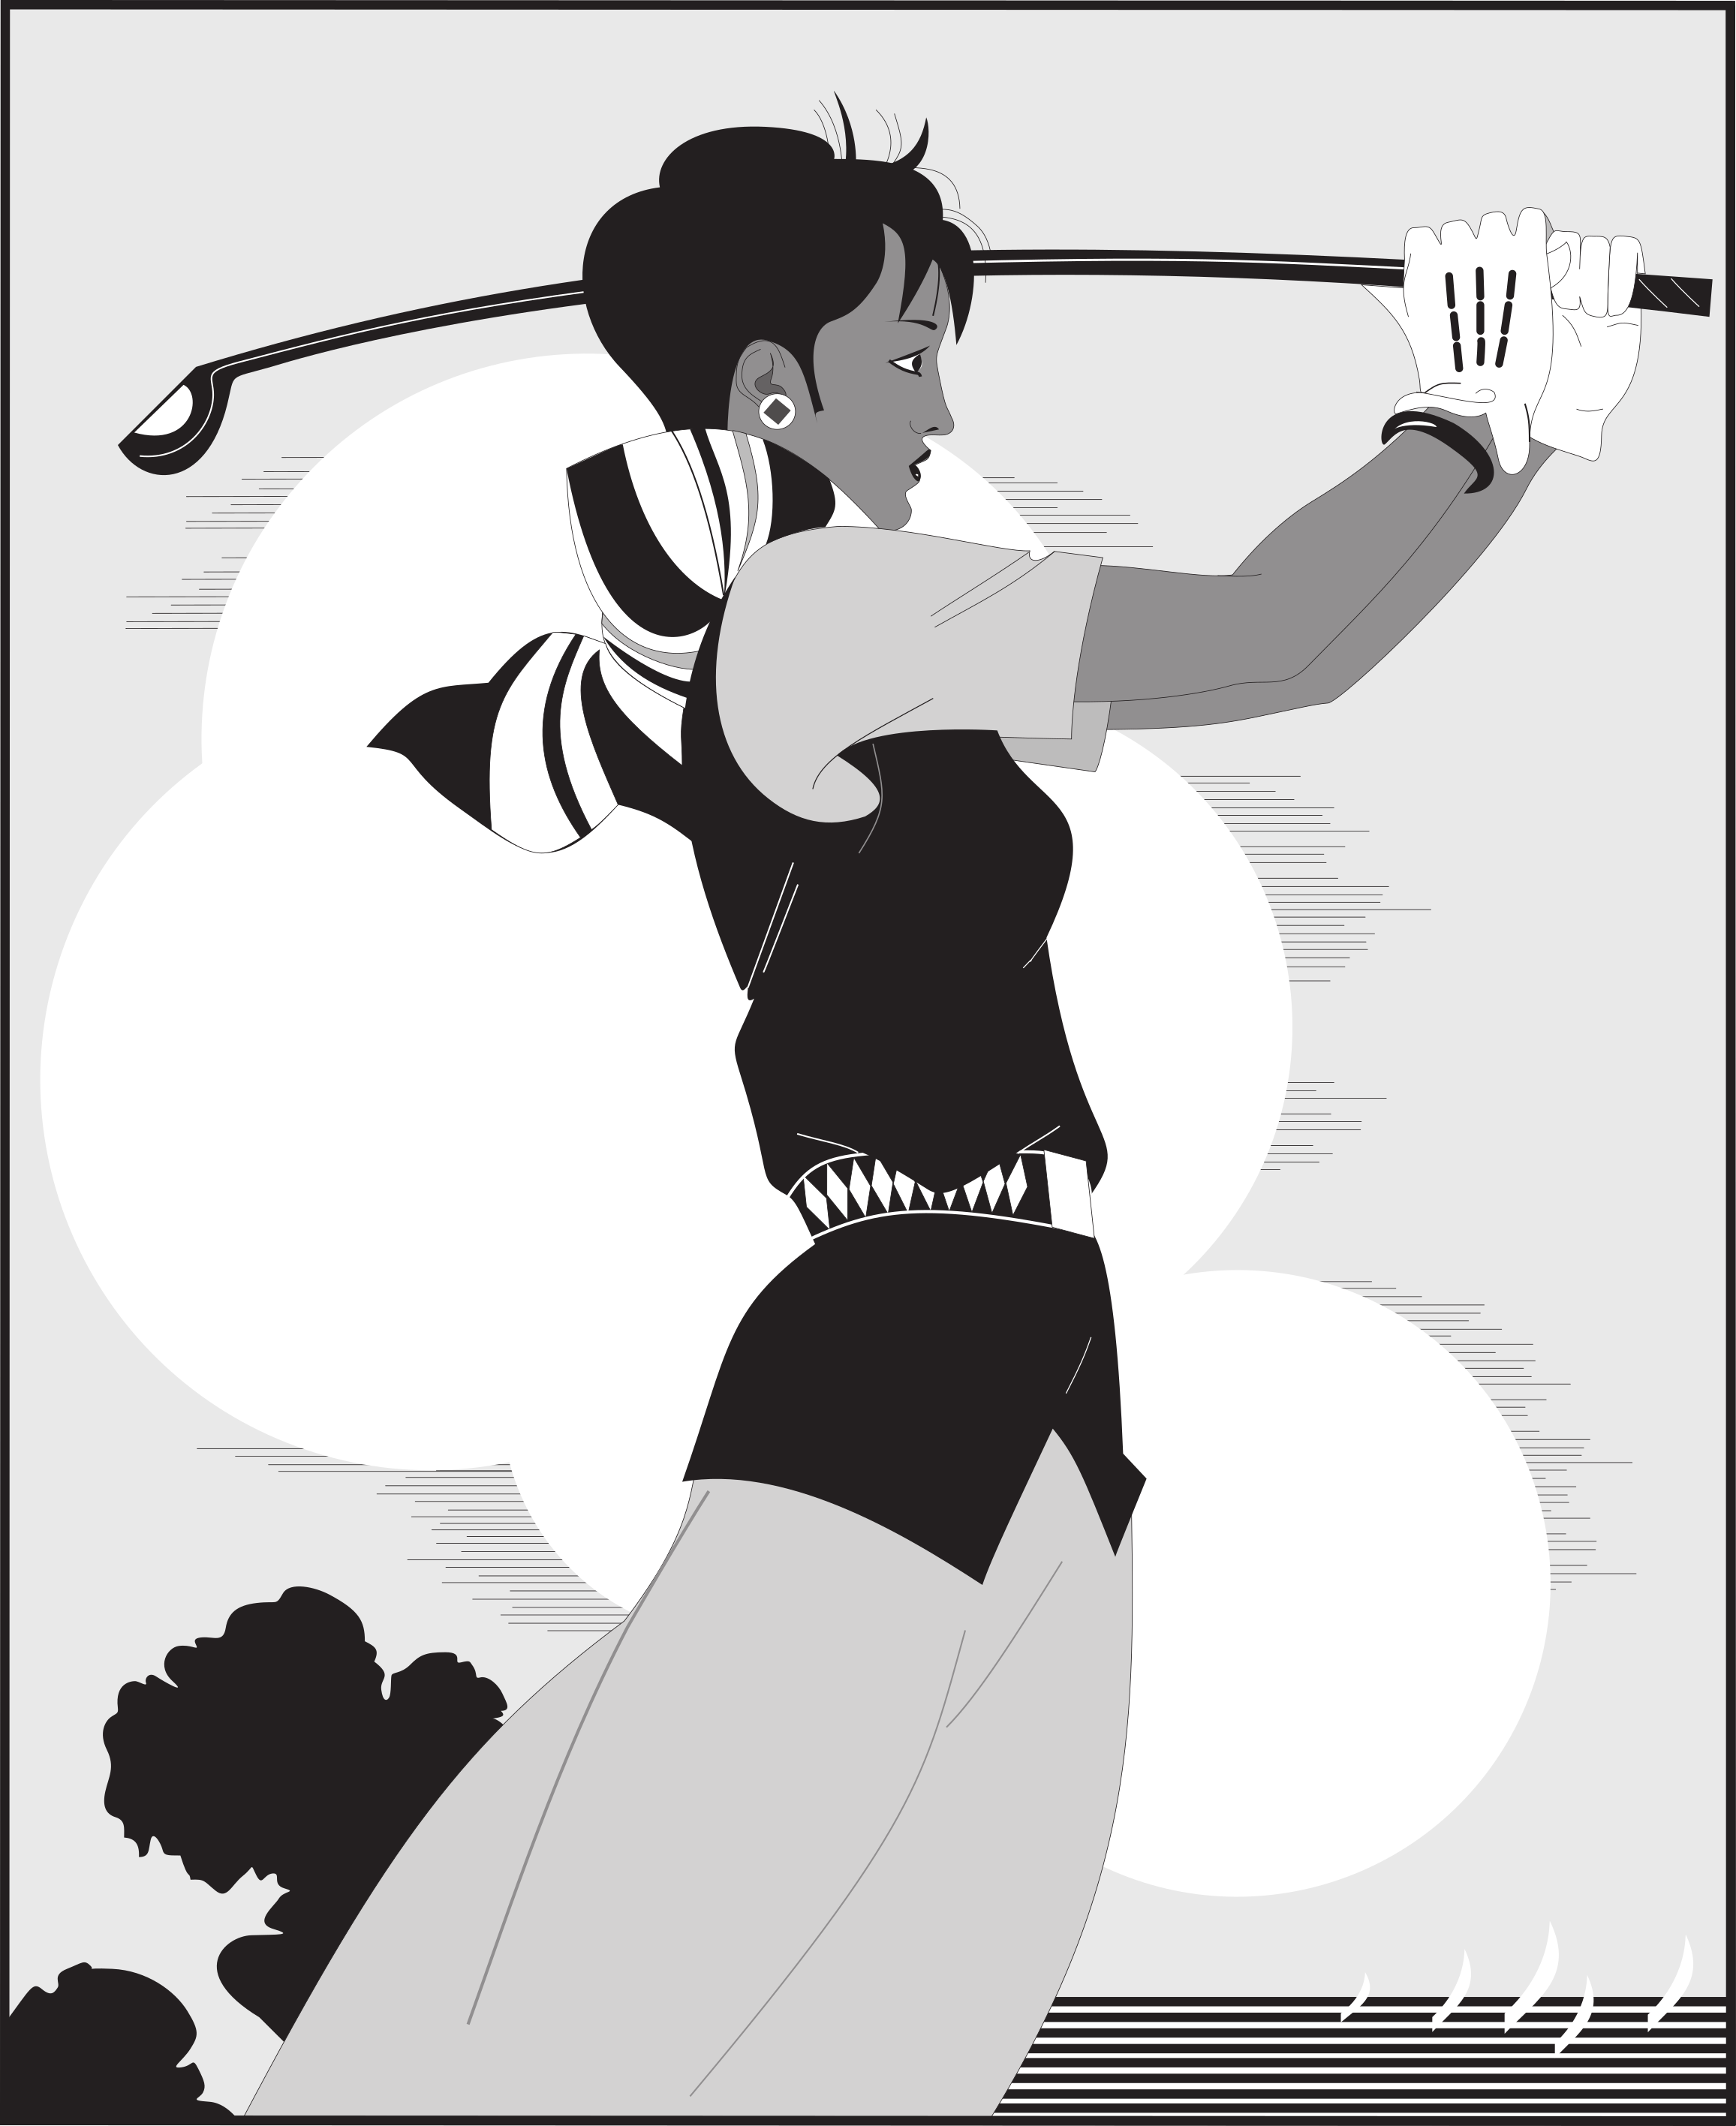
\includegraphics[width = 0.4\textwidth]{golfer}
%\bicaption[golfer5]{}{\xiaosi[0]打高尔夫球的人}{Fig.$\!$}{The person playing golf}\vspace{-1em}
\caption{\xiaosi[0]打高尔夫球的人}
\end{figure}

附录中公式的示例:
\begin{align}
a & = b \times c \\
E & = m c^2
\label{eq}
\end{align}

\chapter{这个星球上最好的免费Linux软件列表}[List of the Best Linux Software in our Planet]
\section{系统}

\href{http://fvwm.org/}{FVWM 自从上世纪诞生以来,此星球最强大的窗口管理器。}
推荐基于FVWM的桌面设计hifvwm:\href{https://github.com/dustincys/hifvwm}{https://github.com/dustincys/hifvwm}。

\subsection{hifvwm的优点}

\begin{enumerate}
	\item 即使打开上百个窗口也不会“蒙圈”。计算机性能越来越强大,窗口任务的管理必须要升级到打怪兽级别。
	\item 自动同步Bing搜索主页的壁纸。每次电脑开机,午夜零点自动更新,用户
		也可以手动更新,从此审美再也不疲劳。
	\item 切换窗口自动聚焦到最上面的窗口。使用键盘快捷键切换窗口时候,减少
		操作过程,自动聚焦到目标窗口。这一特性是虚拟窗口必须的人性化设
		计。
	\item 类似window右下角的功能的最小化窗口来显示桌面的功能此处类似
		win7/win10,实现在一个桌面之内操作多个任务。
	\item 任务栏结合标题栏。采用任务栏和标题栏结合,节省空间。
	\item 同类窗口切换。可以在同类窗口之内类似alt-tab的方式切换。
	\item ……
\end{enumerate}

\section{其他}

\href{https://github.com/goldendict/goldendict}{goldendict 星球最强大的桌面字典。}

\href{https://github.com/yarrick/iodine}{iodine,“HIT-WLAN + 锐捷”时代的福音。}

\href{http://www.aircrack-ng.org/}{aircrack,Wifi“安全性评估”工具。}

\href{https://www.ledger-cli.org/}{ledger,前“金融区块链”时代最好的复式记账系统。}

\href{https://orgmode.org/}{orgmode,最强大的笔记系统,从来没有之一。}

\href{https://www.jianguoyun.com/}{坚果云,国内一款支持WebDav的云盘系统,国内真正的云盘没有之一。}

\href{http://www.mutt.org/}{mutt, ``All mail clients suck. This one just sucks less.''}

\section{vim}
实现中英文每一句一行,以及实现每一句折叠断行的简单正则式,tex源码更加乖乖。
\begin{lstlisting}
vnoremap <leader>fae J:s/[.!?]\zs\s\+/\="\r".matchstr(getline('.'), '^\s*')/g<CR>
vnoremap <leader>fac J:s/[。!?]/\=submatch(0)."\n".matchstr(getline('.'), '^\s*')/g<CR>
vnoremap <leader>fle :!fmt -80 -s<CR>
\end{lstlisting}

%\end{appendix}
%% !Mode:: "TeX:UTF-8" 
\begin{publication}
\noindent\textbf{发表的相关论文}
\begin{publist}
\item	XXX,XXX. Static Oxidation Model of Al-Mg/C Dissipation Thermal Protection Materials[J]. Rare Metal Materials and Engineering, 2010, 39(Suppl. 1): 520-524.(SCI~收录,IDS号为~669JS,IF=0.16)
\item XXX,XXX. 精密超声振动切削单晶铜的计算机仿真研究[J]. 系统仿真学报,2007,19(4):738-741,753.(EI~收录号:20071310514841)
\item XXX,XXX. 局部多孔质气体静压轴向轴承静态特性的数值求解[J]. 摩擦学学报,2007(1):68-72.(EI~收录号:20071510544816)
\item XXX,XXX. 硬脆光学晶体材料超精密切削理论研究综述[J]. 机械工程学报,2003,39(8):15-22.(EI~收录号:2004088028875)
\item XXX,XXX. 基于遗传算法的超精密切削加工表面粗糙度预测模型的参数辨识以及切削参数优化[J]. 机械工程学报,2005,41(11):158-162.(EI~收录号:2006039650087)
\item XXX,XXX. Discrete Sliding Mode Cintrok with Fuzzy Adaptive Reaching Law on 6-PEES Parallel Robot[C]. Intelligent System Design and Applications, Jinan, 2006: 649-652.(EI~收录号:20073210746529)
\end{publist}

\noindent\textbf{(二)申请及已获得的专利(无专利时此项不必列出)}
\begin{publist}
\item XXX,XXX. 一种温热外敷药制备方案:中国,88105607.3[P]. 1989-07-26.
\end{publist}

\noindent\textbf{(三)参与的科研项目及获奖情况}
\begin{publist}
\item	XXX,XXX. XX~气体静压轴承技术研究, XX~省自然科学基金项目.课题编号:XXXX.
\item XXX,XXX. XX~静载下预应力混凝土房屋结构设计统一理论. 黑江省科学技术二等奖, 2007.
\end{publist}
%\vfill
%\hangafter=1\hangindent=2em\noindent
%\setlength{\parindent}{2em}
\end{publication}
    % 所发文章
%\begin{ceindex}
  %如果想要手动加索引,注释掉以下这一样,用wordlist环境
\printsubindex*
\end{ceindex}
    % 索引, 根据自己的情况添加或者不添加,选择自动添加或者手工添加。
%\authorization %授权
%%\authorization[scan.pdf] %添加扫描页的命令,与上互斥
%% !Mode:: "TeX:UTF-8"
\begin{acknowledgements}
衷心感谢导师~高会军~教授和林伟阳副教授对本人的精心指导。他们的言传身教将使我终生受益。感谢姜易木、刘晨璐师兄对我搭建视觉伺服实验环境的帮助和刘海超师兄给我关于特征设计上很棒的启发。感谢霍鑫老师对我控制设计方面的指导和室友武博涵对人机交互界面设计上的大力支持。和一些朋友之间的点点滴滴的交谈中有时也能收获很不错的想法,感谢你们!最后感谢父母和女朋友曹丹琳在我完成毕业设计过程中精神上的莫大支持!


感谢大家,你们每个人的帮助也许只是只言片语,也许重如泰山,但正是所有的这些组成了现在我十分满意的“作品”。

\end{acknowledgements}
 %致谢
%% !Mode:: "TeX:UTF-8" 

\begin{resume}
XXXX~年~XX~月~XX~日出生于~XXXX。

XXXX~年~XX~月考入~XX~大学~XX~院(系)XX~专业,XXXX~年~XX~月本科毕业并获得~XX~学学士学位。

XXXX~年~XX~月------XXXX~年~XX~月在~XX~大学~XX~院(系)XX~学科学习并获得~XX~学硕士学位。

XXXX~年~XX~月------XXXX~年~XX~月在~XX~大学~XX~院(系)XX~学科学习并获得~XX~学博士学位。

获奖情况:如获三好学生、优秀团干部、X~奖学金等(不含科研学术获奖)。

工作经历:

\textbf{( 除全日制硕士生以外,其余学生均应增列此项。个人简历一般应包含教育经历和工作经历。)}
\end{resume}
          % 博士学位论文有个人简介
%%%%%%%%%%%%%%%%%%%%%%%%%%%%%%%%%%%%%%%%%%%%%%%%%%%%%%%%%%%%%%%%%%%%%%%%%%%%%%%% 
% 本科书序为:
%%%%%%%%%%%%%%%%%%%%%%%%%%%%%%%%%%%%%%%%%%%%%%%%%%%%%%%%%%%%%%%%%%%%%%%%%%%%%%%% 
 \authorization %授权
 % \authorization[scan.pdf] %添加扫描页的命令,与上互斥
 % !Mode:: "TeX:UTF-8"
\begin{acknowledgements}
衷心感谢导师~高会军~教授和林伟阳副教授对本人的精心指导。他们的言传身教将使我终生受益。感谢姜易木、刘晨璐师兄对我搭建视觉伺服实验环境的帮助和刘海超师兄给我关于特征设计上很棒的启发。感谢霍鑫老师对我控制设计方面的指导和室友武博涵对人机交互界面设计上的大力支持。和一些朋友之间的点点滴滴的交谈中有时也能收获很不错的想法,感谢你们!最后感谢父母和女朋友曹丹琳在我完成毕业设计过程中精神上的莫大支持!


感谢大家,你们每个人的帮助也许只是只言片语,也许重如泰山,但正是所有的这些组成了现在我十分满意的“作品”。

\end{acknowledgements}
 %致谢
% \begin{appendix}%附录
% \chapter{外文资料的调研阅读报告或书面翻译}

\title{将机器人抓取闭环:一种实时、生成的抓取合成方法}

{\heiti 摘要:} 本文提出了一种实时的、与对象无关的抓取合成方法,可用于闭环抓取。我们提出的生成抓取卷积神经网络 (GG-CNN) 预测每个像素的抓取质量和姿势。这种来自深度图像的一对一映射克服了当前深度学习抓取技术的局限性,避免了抓取候选的离散采样和较长的计算时间。此外,我们的 GG-CNN 在检测稳定抓取的同时具有与当前最先进技术相当的性能,并且数量级更小。我们的 GG-CNN 的轻量级和单通道生成特性允许以高达 50Hz 的频率进行闭环控制,从而在物体移动的非静态环境中以及机器人控制不准确的情况下实现准确抓取。在我们的真实世界测试中,我们在一组先前未见过的具有对抗性几何形状的物体上实现了 83\% 的抓取成功率,在抓取尝试期间移动的一组家用物体上实现了 88\% 的抓取成功率。在动态杂波中抓取时,我们也达到了 81\% 的准确率。

\section{引言}
为了在现实世界的非结构化环境中执行抓取和操作任务,机器人必须能够计算它可能遇到的几乎无限数量的物体的抓取。此外,它还需要能够在动态环境中发挥作用,无论是机器人工作空间的变化、感知的噪声和错误、机器人控制的不准确,还是机器人本身的扰动。


机器人抓取已经研究了几十年,产生了大量不同的技术。最近,深度学习技术在未知项目的抓取合成方面取得了一些最大的进步。这些方法允许学习与超出人工设计特征能力的高质量抓取相对应的特征。


但是,这些方法通常使用为对象识别而设计的卷积神经网络 (CNN) 架构的改编版本 ,并且在大多数情况下,单独对抓取候选对象进行采样和排序 ,导致计算时间较长大约一秒 到几十秒。因此,这些技术很少用于闭环抓取执行,并且依靠精确的相机校准和精确的机器人控制来成功抓取,即使在静态环境中也是如此。
\begin{figure}[h]
	\centering
	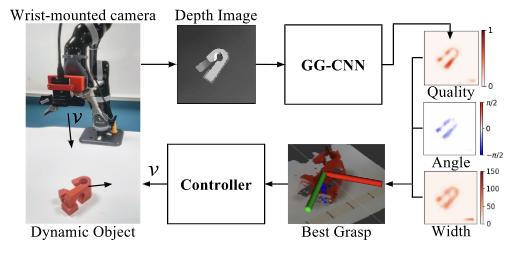
\includegraphics[width=0.8\textwidth]{附录/实时生成抓取管道}
	\caption{实时生成抓取管道。安装在机器人手腕上的摄像头捕捉包含要抓取的物体的深度图像。我们的生成抓取卷积神经网络 (GG-CNN) 为输入图像中的每个像素生成对映抓取——参数化为抓取质量、角度和抓取器宽度在几分之一秒内。计算最佳抓握并向机器人发出速度命令 ($v$)。闭环系统能够抓取动态对象并对控制做出反应。}
	\label{实时生成抓取管道}
\end{figure}


我们提出了一种不同的方法来为以前看不见的项目选择抓取点。我们的生成抓取卷积神经网络 (GG-CNN) 直接为输入深度图像中的每个像素生成对映抓取姿势和质量度量,并且对于动态环境中抓取的闭环控制来说足够快(图 1-1)。我们使用术语“生成”来区分我们的直接抓取生成方法和样本抓取候选的方法。


GG-CNN 相对于其他最先进的合成 CNN 的优势是双重的。首先,我们不依赖于抓取候选的采样,而是直接在像素基础上生成抓取姿势,类似于对象检测的进步,其中全卷积网络通常用于执行像素语义分割,而不是依赖于滑动窗口或边界框 [19]。其次,我们的 GG-CNN 的参数比其他用于抓取合成的 CNN 少几个数量级,这使得我们的抓取检测管道在配备 GPU 的台式计算机上只需 19 毫秒即可执行,速度足以进行闭环抓取。


我们在以下方面评估了我们系统的性能通过使用 Kinova Micorobot 对静态、动态和杂乱的物体进行抓取试验,实现不同的场景。在动态抓取试验中,在抓取尝试期间移动物体,我们在一组 8 个具有对抗几何的 3D 打印物体上实现了 83\% 的抓取成功率 [21],在从标准化对象集中选择的一组 12 个家居用品上实现了 88\% 的抓取成功率。此外,我们重现了 [32] 的动态杂波抓取实验,并显示抓取成功率提高了 81\%。当人为的误差被添加到机器人的控制中时,我们通过报告实验结果进一步说明使用闭环方法的优势。
\section{相关工作}
抓取未知物体抓取合成是指为给定物体制定稳定的机器人抓取方式,这是一个已经被广泛研究的主题,导致了大量的技术。从广义上讲,这些可以分为分析方法和经验方法。分析方法使用几何、运动学和动力学的数学和物理模型来计算稳定的抓取,但由于难以对机械手和对象之间的物理交互进行建模,因此往往不能很好地转移到现实世界中。


相比之下,经验方法侧重于使用模型和基于经验的方法。一些技术适用于已知项目,将良好的掌握点与对象模型或形状或熟悉的项目的离线数据库相关联,基于对象类或对象部分,但无法推广到新对象。


在抓取未知物体方面,最近随着基于视觉的深度学习技术的普及,取得了巨大的进步。许多这些技术共享一个共同的流程:对从图像或点云中采样的抓取候选者进行分类,然后使用卷积神经网络 (CNN) 对它们进行单独排序。一旦确定了最佳抓取候选者,机器人就会执行抓取开环(无需任何反馈),这需要相机和机器人之间的精确校准,机器人的精确控制和完全静态的环境。执行时间是抓取开环执行的主要原因。


在许多情况下,深度学习方法使用具有数百万个参数的大型神经网络 并使用滑动窗口以离散的偏移和旋转间隔处理抓取候选者,这在计算上是昂贵的,并且会导致抓取规划时间大约为一秒到几十秒。

一些方法通过预处理和修剪抓取候选者或同时预测一组离散的抓取候选者的质量来减少执行时间,在执行时间与采样的抓取数量之间进行权衡,但是忽略一些潜在的把握。


与我们的方法类似,Varley 等人,使用神经网络为图像中的手指放置生成像素级热图,但仍然依赖抓取规划器来确定最终的抓取姿势。


我们通过直接同时为图像中的每个像素生成抓取姿势来解决执行时间和抓取采样的问题,使用相对较小的神经网络。


闭环抓取使用视觉反馈将机器人闭环控制到所需姿势通常称为视觉伺服。视觉伺服方法的优点是它们能够适应动态环境并且不一定需要完全精确的相机校准或位置控制。许多工作将视觉伺服直接应用于抓取应用。然而,视觉伺服方法的性质意味着它们通常依赖于手工制作的图像特征来进行对象检测或对象姿态估计,因此不执行任何在线抓取合成,而是收敛到预先确定的目标姿势,并且不适用于未知对象。


最近有人提出基于 CNN 的抓取控制器将深度学习与闭环抓取相结合。两个系统都不是明确地执行抓取合成,而是学习控制器,这些控制器将潜在的控制命令映射到执行控制后的预期质量或距离,需要在每个时间步对许多潜在的命令进行采样。在这两种情况下,控制都以不超过大约 5Hz 的频率执行。虽然两者都是闭环控制器,但动态场景中的抓取仅在一项工作中提出中提出,我们重现了这些实验。


机器人抓取的基准测试由于使用的抓取检测技术范围广泛、对象集之间缺乏标准化以及不同物理硬件(例如机械臂、抓手或相机。许多人报告了对“家庭”对象集的抓取成功率,这些对象在使用的对象的数量和类型上差异很大。

ACRV Picking Benchmark (APB)和 YCBObject Set定义了项目集和操作任务,但在诸如仓库订单履行 (APB) 等任务上进行了基准测试或表格设置和块堆叠 (YCB),而不是通常报告的原始抓取成功率。此外,这两组中的许多项目对于许多机器人和抓手来说都是不切实际的小、大或重,因此尚未广泛用于机器人抓取实验。我们提出了一组 20 个可重复的测试项目,包括 8 个 3D 打印对抗来自的对象和来自 APB 和 YCB 对象集的 12 个项目,它们提供了足够广泛的尺寸、形状和难度,以有效地比较结果,同时不排除任何常见机器人、夹具或相机的使用。

\section{总结}
我们展示了我们的生成抓取卷积神经网络 (GG-CNN),这是一种与对象无关的抓取合成模型,它直接从深度图像以像素为单位生成抓取姿势,而不是像其他深度学习技术那样对单个抓取候选对象进行采样和分类。我们的 GG-CNN 比其他最近的抓取网络小几个数量级,使我们能够以高达 50Hz 的速率生成抓取并执行闭环控制。我们通过抓取试验表明我们的系统能够获得最先进的技术导致抓取未知的动态对象,包括动态杂波中的对象。此外,在存在模拟机器人控制错误的情况下,我们的闭环抓取方法明显优于开环方法。我们通过使用两个标准对象集(一组具有对抗几何的八个 3D 打印对象)来鼓励机器人抓取实验的可重复性。 21]加上来自标准机器人基准对象集的十二个家居用品的建议集,并通过定义我们的动态抓取实验的参数。在我们的两个对象集上,当对象在抓取尝试期间移动时,抓取成功率分别为 83\% 和 88\%,而动态杂波中的对象抓取成功率为 81\%。%本科生翻译论文
% \end{appendix}
%%%%%%%%%%%%%%%%%%%%%%%%%%%%%%%%%%%%%%%%%%%%%%%%%%%%%%%%%%%%%%%%%%%%%%%%%%%%%%%% 
% 博后书序
%%%%%%%%%%%%%%%%%%%%%%%%%%%%%%%%%%%%%%%%%%%%%%%%%%%%%%%%%%%%%%%%%%%%%%%%%%%%%%%% 
% % !Mode:: "TeX:UTF-8"
\begin{acknowledgements}
衷心感谢导师~高会军~教授和林伟阳副教授对本人的精心指导。他们的言传身教将使我终生受益。感谢姜易木、刘晨璐师兄对我搭建视觉伺服实验环境的帮助和刘海超师兄给我关于特征设计上很棒的启发。感谢霍鑫老师对我控制设计方面的指导和室友武博涵对人机交互界面设计上的大力支持。和一些朋友之间的点点滴滴的交谈中有时也能收获很不错的想法,感谢你们!最后感谢父母和女朋友曹丹琳在我完成毕业设计过程中精神上的莫大支持!


感谢大家,你们每个人的帮助也许只是只言片语,也许重如泰山,但正是所有的这些组成了现在我十分满意的“作品”。

\end{acknowledgements}
 %致谢
% % !Mode:: "TeX:UTF-8" 

\begin{doctorpublication}
\noindent\textbf{(一)发表的学术论文}
\begin{publist}
\item	XXX,XXX. Static Oxidation Model of Al-Mg/C Dissipation Thermal Protection Materials[J]. Rare Metal Materials and Engineering, 2010, 39(Suppl. 1): 520-524.(SCI~收录,IDS号为~669JS,IF=0.16)
\item XXX,XXX. 精密超声振动切削单晶铜的计算机仿真研究[J]. 系统仿真学报,2007,19(4):738-741,753.(EI~收录号:20071310514841)
\item XXX,XXX. 局部多孔质气体静压轴向轴承静态特性的数值求解[J]. 摩擦学学报,2007(1):68-72.(EI~收录号:20071510544816)
\item XXX,XXX. 硬脆光学晶体材料超精密切削理论研究综述[J]. 机械工程学报,2003,39(8):15-22.(EI~收录号:2004088028875)
\item XXX,XXX. 基于遗传算法的超精密切削加工表面粗糙度预测模型的参数辨识以及切削参数优化[J]. 机械工程学报,2005,41(11):158-162.(EI~收录号:2006039650087)
\item XXX,XXX. Discrete Sliding Mode Cintrok with Fuzzy Adaptive Reaching Law on 6-PEES Parallel Robot[C]. Intelligent System Design and Applications, Jinan, 2006: 649-652.(EI~收录号:20073210746529)
\end{publist}

\noindent\textbf{(二)申请及已获得的专利(无专利时此项不必列出)}
\begin{publist}
\item XXX,XXX. 一种温热外敷药制备方案:中国,88105607.3[P]. 1989-07-26.
\end{publist}

\noindent\textbf{(三)参与的科研项目及获奖情况}
\begin{publist}
\item	XXX,XXX. XX~气体静压轴承技术研究, XX~省自然科学基金项目.课题编号:XXXX.
\item XXX,XXX. XX~静载下预应力混凝土房屋结构设计统一理论. 黑江省科学技术二等奖, 2007.
\end{publist}
%\vfill
%\hangafter=1\hangindent=2em\noindent
%\setlength{\parindent}{2em}
\end{doctorpublication}
    % 所发文章
% % !Mode:: "TeX:UTF-8" 
\begin{publication}
\noindent\textbf{发表的相关论文}
\begin{publist}
\item	XXX,XXX. Static Oxidation Model of Al-Mg/C Dissipation Thermal Protection Materials[J]. Rare Metal Materials and Engineering, 2010, 39(Suppl. 1): 520-524.(SCI~收录,IDS号为~669JS,IF=0.16)
\item XXX,XXX. 精密超声振动切削单晶铜的计算机仿真研究[J]. 系统仿真学报,2007,19(4):738-741,753.(EI~收录号:20071310514841)
\item XXX,XXX. 局部多孔质气体静压轴向轴承静态特性的数值求解[J]. 摩擦学学报,2007(1):68-72.(EI~收录号:20071510544816)
\item XXX,XXX. 硬脆光学晶体材料超精密切削理论研究综述[J]. 机械工程学报,2003,39(8):15-22.(EI~收录号:2004088028875)
\item XXX,XXX. 基于遗传算法的超精密切削加工表面粗糙度预测模型的参数辨识以及切削参数优化[J]. 机械工程学报,2005,41(11):158-162.(EI~收录号:2006039650087)
\item XXX,XXX. Discrete Sliding Mode Cintrok with Fuzzy Adaptive Reaching Law on 6-PEES Parallel Robot[C]. Intelligent System Design and Applications, Jinan, 2006: 649-652.(EI~收录号:20073210746529)
\end{publist}

\noindent\textbf{(二)申请及已获得的专利(无专利时此项不必列出)}
\begin{publist}
\item XXX,XXX. 一种温热外敷药制备方案:中国,88105607.3[P]. 1989-07-26.
\end{publist}

\noindent\textbf{(三)参与的科研项目及获奖情况}
\begin{publist}
\item	XXX,XXX. XX~气体静压轴承技术研究, XX~省自然科学基金项目.课题编号:XXXX.
\item XXX,XXX. XX~静载下预应力混凝土房屋结构设计统一理论. 黑江省科学技术二等奖, 2007.
\end{publist}
%\vfill
%\hangafter=1\hangindent=2em\noindent
%\setlength{\parindent}{2em}
\end{publication}
    % 所发文章
% % !Mode:: "TeX:UTF-8" 

\begin{resume}
XXXX~年~XX~月~XX~日出生于~XXXX。

XXXX~年~XX~月考入~XX~大学~XX~院(系)XX~专业,XXXX~年~XX~月本科毕业并获得~XX~学学士学位。

XXXX~年~XX~月------XXXX~年~XX~月在~XX~大学~XX~院(系)XX~学科学习并获得~XX~学硕士学位。

XXXX~年~XX~月------XXXX~年~XX~月在~XX~大学~XX~院(系)XX~学科学习并获得~XX~学博士学位。

获奖情况:如获三好学生、优秀团干部、X~奖学金等(不含科研学术获奖)。

工作经历:

\textbf{( 除全日制硕士生以外,其余学生均应增列此项。个人简历一般应包含教育经历和工作经历。)}
\end{resume}
          % 博士学位论文有个人简介
% % !Mode:: "TeX:UTF-8"
\begin{correspondingaddr}
  \heiti\xiaosi
  \noindent 永久通讯地址: \par
  \noindent email: \par
  \noindent 电话: \par
\end{correspondingaddr}
 %通信地址
%%%%%%%%%%%%%%%%%%%%%%%%%%%%%%%%%%%%%%%%%%%%%%%%%%%%%%%%%%%%%%%%%%%%%%%%%%%%%%%% 
\end{document}
% Local Variables:
% TeX-engine: xetex
% End:
